\documentclass[
12pt
,oneside
,openleft         % Moar bigger     % fogs hates this, but they hate everything   % fogs hates this too
]{mythesis}

% I used these in my thesis.  They're useful.  booktabs makes non-shit
% tables.
\usepackage{graphicx}
\usepackage{amsmath}
\usepackage{booktabs}

\title{Phylogenetic models \\%
  of trait evolution}
%
\author{Matthew Wesley Pennell}
%
\month{\textsc{April}} \year{2015}
\previousdegrees{B.Sc., (Hons) Simon Fraser University, 2010}
\degreetitle{Doctor of Philosophy}
\department{Bioinformatics and Computational Biology}

\begin{document}

\maketitle

% I worked in different files: input them like so:

\chapter*{Abstract}
\chaptermark{abstract}
\addcontentsline{toc}{chapter}{Abstract}

One of the most enduring puzzles in evolutionary biology is how processes operating at the level of populations (microevolution) scale up to large-
scale patterns of diversity (macroevolution). Recent advances in our ability to infer the historical pattern of evolutionary branching (the ``phylogeny'') for many groups of organisms have provided opportunities to gain new perspectives on this question. In this dissertation I develop statistical methods, computational machinery, and theoretical frameworks that will enable researchers to make more meaningful inferences about the processes that have driven diversity through deep time using phylogenetic data.

In my opening chapter, I develop a theoretical foundation for how reseachers can use models of trait evolution to test hypotheses related to the long-controversial theory of punctuated equilibrium, which asserts that speciation causes rapid evolution against a backdrop of stasis. I break the hypothesis down into four key elements and argue that combining these conceptually distinct ideas under the single framework of punctuated equilibrium is distracting and confusing, and more likely to hinder progress than to spur it. 

Next, I present a suite of statistical software, written in the R programming language, for fitting evolutionary models to phylogenetic data. This is a complete overhaul of the popular \textsc{geiger} package designed to facilitate analyses of large and complex comparative datasets.

As an example of how phylogenetic models of trait evolution can provide complimentary insights to population-level models, I investigate the evolution of sex chromosome-autosome fusions. Using discrete character models and a recently compiled database of sexual systems, I find that Y-autosome fusions occur at a much higher rate than X-, Z-, or W-autosome fusions in fish and squamate reptiles. This result grounded a theoretical investigation into the evolutionary forces driving sex chromosome fusions---the phylogenetic results allowed my collaborators and I to exclude from consideration several existing theories for why fusions become fixed in populations. Specifically, we found that the phylogenetic results cannot be accounted for by either direct or sexually antagonisitc selection on their own. We argue that the observed patterns can be best explained when chromosomal fusions occur more frequently in males, are slightly deleterious, and are primarily fix by drift.

In the final two chapters, I address two outstanding statistical problems that hinder the use and interpretation of phylogenetic models of trait evolution. First, I develop a novel statistical framework for assessing the absolute fit, or adequacy, of phylogenetic models of trait evolution. To date, researchers have focused almost exclusively on the relative explanatory power of alternative models, rather than the ability of a model to provide a good explanation for data on its own terms. I use my approach to evaluate the statistical performance of commonly used trait models on 337 comparative datasets covering three key functional traits of angiosperms (``flowering plants''). In general, the models I considered often provide poor statistical explanations for the evolution of these traits. This was true for many different groups and at many different scales.  Whether such statistical inadequacy will qualitatively alter inferences drawn from comparative datasets will depend on the context. Regardless, assessing model adequacy can provide interesting biological insights---how and why a model fails to describe variation in a dataset gives us clues about what evolutionary processes may have driven trait evolution across time.

Second, I develop a new technique that leverages taxonomic information to assess and overcome sampling biases in trait datasets; such sampling biases are likely prevalent and have the potential to confound both tests of macroevolutionary and macroecological hypothesis. As an example of the utility of this method, I use it to provide the first estimate of the global distribution of woody and herbaceous plants from a database of 39,313 records and find that the world is likely much woodier than researchers thought. 


%%% Local Variables:
%%% TeX-master: "thesis"
%%% TeX-PDF-mode: t
%%% End:

%\input{preface}
% This is because FoGS formatting pedandtry is especially accute when
% it comes to tables of contents
\allcontents
% There is currently a problem with spacing somewhere so that Table of
% Contents, List of Tables, and List of Figures have the wrong amount
% of space.  Others are OK though...
\chapter*{Acknowledgements}
\addcontentsline{toc}{chapter}{Acknowledgements}

Luke Harmon has been a tremendous mentor, teacher, collaborator, and friend. He came to know me better than I knew myself and found a way to bring out the best in me and restrain the worst. And he made science fun--there is no one else I would rather make mistakes with. 

I thank my committee: Jack Sullivan, for supporting and challenging me in science and in life; Scott Nuismer, for making sure I knew where I stood; Paul Joyce, for always making time when I got stuck on a problem; and Arne Mooers, for introducing me to evolutionary biology and for keeping me honest over the years.

David Tank was practically a second advisor to me. He took me under his wing and taught me how to think and how to be a scientist. And somehow he was able to convince me that plants are actually pretty damn awesome (I will never forget the trips out to Clarkia). He opened new doors for me and fostered new collaborations. I am also thankful to Larry Forney, for always taking the time to talk to me, and for calling me on my bullshit when I needed it.

I thank Simon Uribe-Convers, Brice Sarver, and Tyler Hether for their years of friendship and endless discussions, about biology and everything else. We have experienced all the ups and downs of graduate student life together and through this, they have become like brothers to me.

I have been lucky to have found some incredible people, who I loved hanging out and doing science with (or just hanging out with). Rich FitzJohn and Josef Uyeda have been extremely influential on my intellectual life. They challenged me to think harder and to never take the easy way out. I have learned so much from both of them and enjoyed ever minute (or at least, most) of the many that we spent together brainstorming ideas, writing papers, and hacking code. I also thank Jon Eastman for getting off his rocket ship to help me whenever I fell off my tricycle. And David Bapst has been my constant sounding board and sparring partner throughout my dissertation. It is only because of him that I can converse with paleontologists without complete embarrassment.

A huge number of people have reached out and guided me in a myriad of ways. Their intellectual and personal generosity is truly humbling. I would particularly like to thank Michael Alfaro, Steve Arnold, Will Cornwell, Bernie Crespi, Joe Felsenstein, David Green, Paul Harnik, Mark Kirkpatrick, Craig Miller, Brian O'Meara, Sally Otto, Erica Bree Rosenblum, Graham Slater, David Swofford, and Amy Zanne.

It has been an incredible privilege to do science in the Harmon/RoHa lab; you guys are the best. I thank James Rosindell, Joseph Brown, Jamie Voyles, Suzanne Joneson, Travis Hagey, Simone Des Roches, Tom Poorten, Kayla Hardwick, Denim Jochimson, Kayla Hardwick, Daniel Caetano, Rafael Maia, and Eliot Miller.

I loved being an IBESTian at the University of Idaho. I am thankful to all the people who made it so fun, both in and out of the office. In particular, I would like to thank Diego Morales-Briones, Sarah Jacobs, Hannah Marx, Daniel Beck, Genevieve Metzger, CJ Jenkins, Matt Singer, Michael France, Luke Caldwell, Chloe Stenkamp-Strahm, Sam Hunter, Matt Settles, Anahi Espindola, Matthieu Delcourt, and Wesly Lofte-Eaton. I thank all the IBEST staff and faculty, especially Lisha Abendorth and Eva Top, for without their boundless patience, I would literally not have finished my Ph.D.

I thank Roxana Hickey for all the things--for celebrating with me when things were going well; for commiserating when things were not; for listening to me rant even when she didn't care; for being my friend; for suffering me when I was insufferable; and for always pushing me to be better. Last, I would like to thank my family: my parents, Rick and Brenna Pennell, and my siblings, Stephen, Alec, and Laura. I cannot even begin to articulate the support they have given me over the years nor my gratitude for it. For once, I have no words.


%%% Local Variables:
%%% TeX-master: "thesis.tex"
%%% TeX-PDF-mode: t
%%% End:

\cleardoublepage
\phantomsection
\addcontentsline{toc}{chapter}{Dedication}
\vspace*{200pt}
\begingroup
\begin{center}
\large\textsc{Dedication}\\
\bigskip
\textit{To my grandparents}\\
Betty and Joseph Pennell\\
Frieda and Earl Harder
\end{center}
\endgroup
\vspace*{\fill}

\cleardoublepage
\mainbody

\chapter[Introduction: Models, meanings, and macroevolution]{Introduction: Models, meanings, and macroevolution \footnote {This chapter was previously published in a modified form as: Pennell M.W. 2015. Modern Phylogenetic Comparative Methods and Their Application in Evolutionary Biology: Concepts and Practice--Book Review. Systematic Biology 64:161--163}}
\label{chap:introduction}

\section{Objectives and structure of this dissertation}

The primary goal of my dissertation is to improve the statistical and conceptual foundations that underlie phylogenetic tests of macroevolutionary hypotheses. To address the statistical component, I have: led the development of statistical software for fitting models and analyzing data (\spacedsmallcaps{\Chapref{geiger}}), which I used to study the macroevolution of sex chromosomes across vertebrates (\spacedsmallcaps{Chapter 4}); created a novel framework for assessing the  absolute fit, or adequacy, of models of trait evolution (\spacedsmallcaps{Chapter 5}); and developed a new approach for evaluating and dealing with sampling biases in comparative datasets (\spacedsmallcaps{Chapter 6}), a problem that is becoming increasingly pertinent, if understudied, as researchers rely more on curated collections of data. Additionally, I have been involved in a number of other projects during my Ph.D. (not included in this dissertation) in which I have examined the statistical properties of existing phylogenetic comparative approaches \citep{Pennell2012, UyedaPCA, Sarverprior}, developed new ones \citep{SlaterPennell, ksi} and applied these to test empirical questions in angiosperms \citep{ksi, nestedradiations} and ascidians \citep{Maliska2013}.

As mentioned above, I have coupled my work in statistical methods with more theoretical work, in which I aimed to provide roadmaps for better interpreting the results of tests using these methods \citep{Rosenblum2012, PennellHarmon, PennellPE, PennellTREEresponse, Pennellpcmbook}. One of these projects, an investigation into tests of the theory of punctuated equilibrium \citep{Eldredge1971, EldredgeGould1972} is included as a chapter in this dissertation (\spacedsmallcaps{Chapter 2}). 

As an introduction to my dissertation, I briefly overview the field of comparative biology \citep[for a more comprehensive discussion, see][]{PennellHarmon} and point out what I believe is the biggest challenge facing the field--that we often have a poor understanding of precisely what we are measuring and explaining when we use phylogenetic comparative methods (PCMs)--and highlight possible ways forward.

\section{Overview of phylogenetic comparative methods}

Investigating similarities and differences across species (the ``comparative method'') has been an esssential conceptual tool in the study of adaptation since \citet{Darwin1859}. Interspecific comparisons are especially valuable when there is little or no variation in the trait of interest within species; in these cases, complimentary approaches such as field experiments are of limited utility. Even when there is variation within a species, the comparative approach allows biologists to assess the generalities of patterns. PCMs for the study of adaptation arose out of the recognition that shared evolutionary history can confound statistical comparisons \citep{HarveyPagel1991}. As a result of the process of descent with modifications, closely related species share many traits and trait combinations and therefore individual species cannot be considered independent observations. In the 1980s and early 1990s, a number of highly influential statistical approaches were developed to incorporate phylogeny into interspecific comparisons \citep{Ridley1983, Felsenstein1985, Grafen1989, Maddison1990, HarveyPagel1991, Lynch1991, Pagel1994}. 

While initially controversial \citep[e.g.,][]{Westoby1995}, PCMs have gained near universal acceptance in the ensuing decades, such that today, it is near impossible to publish an interspecific study without considering phylogeny. This victory for phylogenetics is so decisive that some researchers have expressed concern that the pendulum has swung too far toward phylogenetic approaches in the study of evolutionary ecology \citep{Losos2011}. While PCMs are still routinely used to test for adaptation, the field has evolved in subtle yet substantial ways: researchers recognized that the same models developed for comparative questions could also be used to test macroevolutionary questions--for example, what is the pattern of trait change through deep time and what processes drove these trends?--that were long the exclusive domain of paleobiology \citep{HansenMartins1996, Hansen1997, Schluter1997, Pagel1997, MooersSchluter1998, Pagel1999, Mooers1999}. The rate of development of novel PCMs has been incredible and this pace has been matched by the ever-increasing availability of more reliable phylogenetic trees along with large-scale efforts to aggregate phenotypic data from across the Tree of Life.

\section{Current challenges in comparative biology}

Despite the incredible progress of phylogenetic comparative methods over the last few decades, there remain some fundamental issues that are deeply unsettling: while we have sophisticated machinery for fitting many different types of models to comparative data, we often lack a clear interpretation of what exactly they mean. Reading many papers in the field (including my own!), I cannot help but recall a sentiment expressed by \citet{Houle2011} in their lucid review of measurement theory and its applications in biology. They criticize statisticians who advocate that data transformations are justifiable whenever they result in distributions that meet the assumptions of a particular analysis: ``If that is statistics, we want no part of it, as science is about nature, not numbers'' [p. 18]. I argue that our ability to analyze phylogenetic comparative data has outpaced our ability to understand it.

Consider for example, regression models of the form
\[Y=\beta_{\text{0}} + \beta_{\text{1}}X + \epsilon.\]
In phylogenetic regression \citep{Grafen1989, Lynch1991}, it is usually assumed that the tree only enters into the model in the error term $\epsilon$ such that $\epsilon \sim \mathcal{N}(\textbf{0}, \mathbf{V})$ where $\mathbf{V}$ is the expected variance-covariance matrix for the traits given an evolutionary model. In other words, the evolutionary model is used to model the structure of the residuals and not the actual traits. Formulating the model in such a way allows us to make use of well-established statistical theory from generalized least squares (GLS) and generalized linear mixed-effects (GLM) models \citep{Lynch1991, Rohlf2001, Rohlf2006, Housworth2004, Hadfield2010}. Including the phylogenetic structure in the error variance is no different from including any other type of covariance. By recognizing this equivalency, we can now fit phylogenetic regression models with a variety of distributions for the response variable $Y$ \citep{Ives2010, Hadfield2010}, incorporate measurement error \citep{Ives2007, Hansen2012SysBio}, and take advantage of a large number of other standard statistical tricks \citep[see][for a recent review]{PCM}

There are a variety of different models one can use to create $\mathbf{V}$. The most popular is to assume that the residuals are distributed according to the expectations of a Brownian motion (BM) model. Indeed, the original independent contrasts method \citep{Felsenstein1985} produces identical results to a phylogenetic regression model when this assumption is made \citep{Blomberg2012}. A number of the researchers have advocated that a $\lambda$ tree transformation \citep{Pagel1999, Freckleton2002, Freckleton2011} is often more appropriate than simply assuming BM for constructing the error variance term $\mathbf{V}$. (The $\lambda$ transformation involves multiplying the off-diagonals of $\mathbf{V}$ by a estimated parameter between 0 and 1.) This is a purely phenomenological construct--by shrinking every branch except those leading to the tips, it implies that there is something special about extant taxa, which is clearly not the case. Nonetheless, researchers often use such models to claim that one trait is adapted to the value of another. In a series of papers, Hansen and colleagues have clearly articulated the problem with such inferences \citep{HansenOrzack2005, Hansen2008, Labra2009, Hansen2012SysBio}. Effectively, standard regression models assume adaptation to a new environment is instantaneous and that maladaption is phylogenetically structured; closely related species will have similar deviations from the optimal trait value even if the optimum differs between them. From a biological perspective, this seems very odd.

Perhaps even more confusing is the use of Ornstein-Uhlenbeck (OU) models to construct the error variance term. OU is attractive for modeling the residual variance because, unlike the $\lambda$ transformation, it is a coherent stochastic process and is directly analagous to a population level model from quantitative genetics--quadratic stabilizing selection on a fixed adaptive landscape \citep{Lande1976, HansenMartins1996}. While the $\lambda$ transformation is obviously just a statistical construct, OU \emph{seems} biologically motivated. Indeed, researchers commonly interpret the OU-structured variance term as representing stabilizing selection or constraints. But these does not get around Hansen's criticisms. These models still assume phylogenetically structured maladapation and they do they allow researchers to make specific inference about stabilizing selection or evolutionary constraints--it is completely unclear precisely what is being constrained or how the residuals are under stabilizing selection. OU error structures may often fit data better than BM error structures but it is likely that this is simply because OU can accomodate more variance towards the tips of the phylogeny than a BM model can (including $\lambda$ has a similar effect). The evolutionary argument here seems merely window dressing for a purely statistical argument. 

The arguments I have made here apply equally well to models without predictor variables--where what we want to explain with comparative methods are the distribution of traits through time without considering predictor variables. It is now a common exercise in both phylogenetic comparative biology and paleobiology to compare alternative models of trait evolution and then to interpret the best-fitting model in terms of evolutionary processes \citep[e.g.,][]{Mooers1999, Hunt2007, Harmon2010, Hopkins2012, Burbrink2012, Hunt2012}

\section{Paths forward}

How then are we to make sense of comparative analyses? In my view, there are three possible frameworks with which to think about comparative biology. First, we can take the view that what we are measuring are strictly patterns and that we are not necessarily making inferences about specific evolutionary processes. This is certainly a defensible position: the patterns may be interesting in and of themselves and documenting commonalities and differences among clades and through time may provide a broader picture of the history of life on earth. In practice, this is what researchers are often actually doing, even if they are hesitant to admit this. And since the models we used in comparative biology predict trait distributions that conform to common probability distributions, there are undoubtedly a huge number of processes that could generate the patterns we observe \citep{Jaynes2003, Frank2009, Frank2014}.
A benefit of openly adopting this perspecitve is that we can consider a much broader suite of models that may provide a much better fit to our data and predictive power than current models--if we are not interested in making specific evolutionary inferences, then we need not be beholden to specific evolutionary models. Such alternatives may include macroevolutionary diffusion processes \citep[e.g.,][]{Clauset2008}, models derived from macroecological theories \citep{Brown2004, Harte2011} or making use of statistical learning approaches divorced from any process whatsoever.

The second framework is the quantitative genetics view: the models we fit in comparative biology should be taken as literally representing microevolutionary hypotheses. Many of the commonly used models can be directly interpreted in terms of population-level parameters \citep{HansenMartins1996, PennellHarmon}. We can compare the estimated model parameters to within-population measures to test if macroevolutionary divergences are consistent with evolution by drift, stabilizng selection, etc. This project is certainly interesting and worth pursuing. But given the results of studies that have explicitly examined this connection \citep{Lynch1990, EstesArnold2007, Hohenlohe2008, Harmon2010, Bolstad2014} using rather simple models, it appears that translating the parameters estimated from comparative data to the terms of quantitative genetics (e.g., if we assume that BM is strictly a model of drift with fixed additive genetic variance $\mathbf{G}$, the estimated rate parameter $\sigma^2$ is equal to $\mathbf{G}$ divided by the effective population size $N_e$ ; \citealt{Lande1976}) will often result in nonsensical numbers. 

The third perspective is to take seriously the idea that macroevolutionary models reflect the dynamics of adaptive landscapes through deep time \citep{Arnoldetal2001, Hansen2012book, PennellPE}. Comparative biologists have a tendency to discuss many of these ideas in scare quotes. The optimum of OU models is referred to as ``clade level optimum''. A model with decelerating rates of change depicts an ``early burst''. I argue that a much richer and more meaningful connection can potentially be made. Theoretical work over the last century has produced a beautiful and fairly comprehesive understanding of how populations move across adaptive landscapes and empricists have tested the theoretical predictions in a wide variety of systems and contexts. In contrast, we have only a preliminary understanding of how the landscapes themselves evolve on longer time scales. This is a fundamentally important question in evolutionary biology and one which I believe, phylogenetic comparative biology and paleobiology can help address. 

There is a lot of work to be done before we will really able to get at these types of questions. Once we recognize that some of the classic concepts in evolutionary biology--such as adaptive zones, adaptive radiations and key innovations--are actually hypotheses about the structure and dynamics of adaptive landscapes \citep{Hansen2012book}, we can start developing statistical models that actually capture their essential properties. Current models are, at best, loosely tied to these ideas (hence the scare quotes). Additionally, there are a number of exisiting mathematical frameworks that make predictions about these higher order processes and trait evolution over longer time periods \citep[see for example,][]{Holt2003, Gavrilets2004, Doebeli2011}. But there is currently no way to estimate the relevant parameters of these models from comparative data.  

\section{Concluding remarks}

Both the development of new PCMs and the interest in using them has grown tremendously over the last decade.  Nevertheless, I feel that we, as a field, are somewhat stuck. First, the same handful of statistical models are employed over and over again with most of the progress representing relatively minor variations on similar themes. (That is not the say that such improvements are not challenging or worthwhile; indeed a portion of my dissertation is aimed in precisely this direction.) Second, we are often much too vague on what exactly we want to explain with PCMs--this is apparent in both this current collection and in the literature more broadly. I argue that these two problems are deeply intertwined. The standard collection of models available today, namely those based on BM and OU, have had such staying power in part because they can be useful for detecting patterns, can be interpreted in light of evolutionary genetics and can loosely be tied to questions about adaptive landscapes. Requiring this sort of conceptual flexibility is also a limitation. More focused, question-specific approaches to modeling that are directly tied to the inferences we actually want to make will likely get us much further than sticking to models that are more general but address no questions particularly well.

 

   

%%% Local Variables:
%%% TeX-master: "thesis"
%%% TeX-PDF-mode: t
%%% End:

\chapter[Revisiting the punctuated equilibrium debate in light of emerging phylogenetic data and methods]{Revisiting the punctuated equilibrium debate in light of emerging phylogenetic data and methods\footnote{Previously published as: Pennell, M.W., L.J. Harmon, and J.C. Uyeda. 2014.
  Is there room for punctuated equilibrium in macroevolution?
  Trends in Ecology \& Evolution 29:23--32}}
\label{chap:punceq}

\section{Summary}

The long-controversial theory of punctuated equlibrium (PE) asserts that speciation causes rapid evolution against a backdrop of stasis. PE is currently undergoing a resurgence driven by new developments in statistical methods. However, we argue that PE is actually a tangle of four unnecessarily conflated questions: i) is evolution gradualistic or pulsed?; ii) does trait evolution occur mainly at speciation or within a lineage?; iii) are changes at speciation adaptive or neutral?; and iv) how important is species selection in shaping patterns of diversity? We discuss progress towards answering these four questions but argue that combining these conceptually distinct ideas under the single framework of PE is distracting and confusing, and more likely to hinder progress than to spur it.


\section{Introduction: the resurgence of punctuated equilibrium}

The following three quotations were all drawn from abstracts of recent papers purporting to use statistical models to empirically evaluate punctuated equilibrium (PE):

\begin{quote}
\singlespacing
A long-standing debate in evolutionary biology concerns whether species diverge gradually through time or by punctuational episodes at the time of speciation. We found that approximately 22\% of substitutional changes at the DNA level can be attributed to punctuational evolution, and the remainder accumulates from background gradual divergence. \citep[][p. 119]{Pagel2006}
\end{quote}

\begin{quote}
\singlespacing
This controversy, widely known as the `punctuated equilibrium' debate, remained unresolved, largely owing to the difficulty of distinguishing biological species from fossil remains. We analyzed body masses of 2143 existing mammal species on a phylogeny comprising 4510 (i.e. nearly all) extant species to estimate rates of gradual (anagenetic) and speciational (cladogenetic) evolution. \citep[][p. 2195]{Mattila2008}
\end{quote}

\begin{quote}
\singlespacing
Under such processes, observations at the tips of a phylogenetic tree have a multivariate Gaussian distribution, which may lead to suboptimal model specification under certain evolutionary conditions, as supposed in models of punctuated equilibrium or adaptive radiation. \citep[][p. 193]{Landis2012}
\end{quote}
These three papers are representative of a substantial number of other recent high-profile studies that have discussed their research in the context of PE \citep[e.g.,][]{Hunt2007, Hunt2008, Huntetal2008, Webster2003, Bokma2002, Bokma2008, Ingram2011, Uyeda2011, Rabosky2012, Hunt2012, Bartoszek2013, Rabosky2013, Simpson2013, Atkinson2008, Baca2013}. This is somewhat remarkable given that arguably no idea has had such a turbulent history in modern evolutionary thought as punctuated equilibrium. In the early 1970s, Eldredge and Gould \citep{Eldredge1971, EldredgeGould1972, GouldEldredge1977} proposed that the predominant pattern of evolution throughout deep time is that of stasis ``punctuated'' by brief intervals of rapid evolution, which often occurred during speciation events. This was originally conceived as a way of bridging the gap between prevailing ideas about speciation, i.e., Mayr's allopatric model \citeyearpar{Mayr}, and observations from the fossil record \citep{Sepkoskibook}. However, PE has expanded and shifted in definition to become a much more far-reaching hypothesis to many researchers. Consequently, it has been viewed as both a a rather innocuous statement about the general patterns found in the fossil record and as an affront to the central tenets of evolutionary theory \citep{Stanley1975, Stanley1979, Gould1980, Charlesworth1982, Levinton2001}. For some researchers, the stakes of the debate over the prevalence of PE could not have been higher:

\begin{quote}
\singlespacing
If most evolutionary changes occurs during speciation events, and if speciation events are largely random, natural selection, long viewed as the process guiding evolutionary change, cannot play a significant role in determining the overall course of evolution. Macroevolution is decoupled from microevolution... \citep[][p. 648]{Stanley1975}
\end{quote}

In the wake of such claims, much of the intellectual history of PE was been characterized by fierce, and often vitriolic, theoretical debates--exhaustively catalogued in \citep{Levinton2001, Gould2002}--and the theory remains divisive \citep[for more on the history of the idea, see][]{Sepkoskibook}.

The field of macroevolution has recently witnessed a resurgence of interest in PE as paleobiologists and, increasingly, comparative biologists armed with molecular phylogenies, have applied sophisticated statistical models to quantitatively test the major hypotheses of PE. In this review, we ask whether these new statistical advances have ``rescued'' PE from intellectual extinction. We answer this question in the negative. The challenges inherent in elucidating macroevolutionary processes and patterns from paleontological and comparative data are only exacerbated by the muddled historical legacy of PE. Although a number of studies have indeed discussed their findings in light of PE, they have actually addressed a wide variety of conceptual issues; the studies from which we have quoted above exemplify this--each one asks a fundamentally distinct question.

What then, exactly, defines PE? The central definitions and concepts of PE have shifted substantially over time--including the views of the theory's chief advocates \citep{Mayr1982, Ruse1989, Sepkoskibook}. We argue that the key to disentangling this Gouldian knot, lies not in attempting to parse the literature in search of the true ``essence'' of PE, but rather in recognizing that the myriad concepts often associated with the theory can be conceptually dissociated and evaluated independently. We believe that dissociating the different components of PE will lead to a more productive discussion of these ideas and facilitate progress in some of the most fundamental questions in macroevolution. In this essay, we identify four key questions that have been lumped under the topic of PE, discuss how their association with each other has led to confusion, and comment on recent methodological developments, using a variety of types of data, that may provide novel insights into large-scale patterns of diversity.

\section{Punctuated equilibrium as a conglomerate of concepts}

In our view, the theory of PE, and the extensive discussion surrounding it, conflates four separate primary research questions: i) what is the relative importance of gradualistic versus pulsed evolution?; ii) what is the role of speciational events (cladogenesis) vesus within lineage evolution (anagensis) in generating trait divergence?; iii) when change is cladogenetic, are these changes adaptive or driven by neutral processes?; and iv) how important is higher level selection (species selection) in shaping patterns of diversity? 

\subsection{Gradualistic versus pulsed evolution}

In principle, it is quite feasible to distinguish gradualistic versus pulsed evolution using either phylogenetic comparative or paleontological data. Constant-rate gradualism is typically modeled as a random walk or Brownian motion process in both phylogenetic and paleobiological studies (BM; see \textsc{box 1}). Several recent studies have examined whether fossil time-series conform better to predictions from constant-rate BM, phenotypic stasis, or directional evolution, which each predict different distributions of trait values through time and can be distinguished using model selection techniques \citep{Hunt2012}. These studies have found mixed support for each mode of evolution in different lineages and traits \citep{Hunt2007, Huntetal2008, Hunt2008, Grey2008, Hopkins2012, Hunt2012}. An exceptional demonstration of pulsed evolution in the fossil record was examined by \citet{Huntetal2008}, who found support for a rapid pulse of evolution in sticklebacks as they colonized a novel adaptive peak. Similar model-fitting approaches have been used to demonstrate that in particular fossil time-series shifts in the mode of evolution (i.e., directional evolution, stasis, or BM) are separated by phenotypic bursts \citep{Hunt2008}. This pulsed pattern of evolution is supported by large collections of micro- and macroevolutionary data \citep{EstesArnold2007, Uyeda2011}. Studies of fossil time-series often include a number of caveats that may complicate inference of evolutionary modes. These include unequal sampling probabilities and uncertain stratigraphic position, as well as issues relating to range shifts, time-averaging and phenotypic plasticity \citep{StratPaleobook}. A particularly promising, albeit data-intensive, method developed by \citet{Hannisdal2007} incorporates some of these additional sources of uncertainty in a Bayesian framework.

While fossil time-series provide direct observations of phenotypes over time, they are limited by the difficulty in confidently assembling sequences of ancestor-descendant relationships. Phylogenetic comparative methods provide a complementary means to study departures from constant-rate gradualism; these can be applied to both extant and extinct data, if the fossil data can be placed in a phylogenetic context \citep{PennellHarmon}. Several methods allow the detection of rate shifts across clades by allowing the BM rate parameter $\sigma^2$ to differ across branches of the phylogeny \citep[e.g.,][]{Omeara2006, Eastman2011, Slater2012MECCA}. However, these methods model sustained shifts in evolutionary rates, rather than pulsed patterns suggested by PE. Pure-burst models, in which all change accumulates in pulses, can also be fit to phylogenies and more closely align with PE \citep{HansenMartins1996, Khaitovich2005, Uyeda2011}. \citet{Landis2012} developed a particularly promising approach that models both gradual and punctuational patterns of evolution using jump-diffusion models, in which both jumps and gradual evolution come from a single, long-tailed distribution \citep[see also,][]{Eastmanjump}. In addition to these methods, discrete shifts in adaptive optima separated by long periods of stabilizing selection have been extensively implemented in in phylogenetic comparative methods by using Ornstein-Uhlenbeck (OU) models \citep{Felsenstein1988, Hansen1997, ButlerKing2004}. OU models are attractive alternatives to BM that can incorporate stasis, stabilizing selection and adaptive hypotheses \citep[][see \textsc{box 1} for further details]{PennellHarmon}. 

Advances in quantitative model-fitting of evolutionary processes have allowed us to explore much wider range of evolutionary hypotheses and processes than simple BM \citep{PennellHarmon}, including pulsed evolutionary patterns. However, to what extent does the framework of punctuated equilibrium contribute to interpretation of the results of these models? Note that none of the models described in this section can distinguish between cladogenetic or anagenetic change (see next section). Furthermore, PE is tied to a very specific pattern of evolution and a specific temporal frame: stasis over the lifespan of a species (typically millions of years) followed by geologically brief bursts of phenotypic evolution occurring at speciation \citep{EldredgeGould1972, GouldEldredge1977, Gould2002}.  Therefore, even robust support for a pattern of pulsed evolution--represented by shifts in trait values along branches that are not accounted for by gradual evolution--may be incompatible with PE if the pulses occur too infrequently for conventional PE theory, which predicts pulses at all (or nearly all) speciation events. In addition, exactly as paleontologists have long recognized that repeated burst-stasis episodes can appear gradualistic if viewed at too coarse a scale, gradualistic evolution with variable rates can appear pulse-like at the same coarse scale. A pulsed pattern detected from phylogenies--which typically have much longer timescales and coarser sampling than a fossil time-series, may not reflect phenotypic bursts between species. Instead, model-fits may reflect ``jumps'' between higher-level niche space or adaptive zones, within which whole clades or groups of species may cluster \citep{Simpson1944, Hansen1997, Hansen2012book, Eastmanjump}. The observation that groups of species cluster around different phenotypic optima says nothing about whether individual lineages exhibit a pattern of stasis and phenotypic bursts of evolution over the lifespan of individual species. Tying patterns measured at phylogenetic scales to species-level and not clade-level change is fraught with difficulty. However, we can still address other interesting macroevolutionary questions such as whether evolution is characterized by pulses, how often they occur and what ecological factors may be associated with them \citep{Eastmanjump}.

\subsection{Anagenetic versus cladogenetic change}

Although speciation is undoubtedly associated with genetic and trait divergence \citep[][and references therein]{Nosil2012}, its relative importance compared to evolutionary change within a lineage is currently poorly understood. Several studies have attempted to evaluate the contribution of cladogenetic change to trait evolution \citep{WagnerErwin1995, JC1999, Aze2011, Strotz2013} using paleontological data. This is evaluated by determining whether the stratigraphic ranges of descendant species overlap with their progenitor species, indicative of coexistence and cladogenesis. However, robustly distinguishing between cladogenetic and anagenetic changes using fossil data crucially depends on several assumptions, such as the accurate reconstruction of ancestor-descendant relationships, the equivalency of species concepts applied to fossil and extant taxa, the robust estimation of species' temporal ranges and enough sampling to eliminate the possibility of gradual evolution \citep{JC1999}. Disputes over the validity of these assumptions have been well played out in the punctuated equilibrium literature \citep[e.g., the Turkana Basin molluscs,][]{Williamson1981, Fryer1983, VanBocxlaer2008}. Approaches have been developed to account for potential biases, such as estimating ancestor-descendant relationships \citep{Marshall1995, Foote1996} and stratigraphic ranges \citep{Marshall1990, Marshall1994, Marshall1997, Wagner2000}, accounting for sampling, but difficulties remain.  As a recent example, \citet{Strotz2013} found a predominance of cladogenetic change among fossil Foraminifera, using assumed ancestor-descendant relationships assembled from stratigraphic and phenotypic data \citep{Aze2011}. We view such claims with considerable skepticism because it is impossible to detect cryptic speciation--which is increasingly being inferred in extant groups \citep{Fujita2012}--in the fossil record, and therefore distinguish decisively between anagenetic and cladogenetic change.

Another tactic to assess the relative contributions of anagenetic and cladogenetic change has been to look for correlations between speciation rates (or species richness, as a proxy for speciation rates) and rates of evolution using phylogenetic comparative data. This has been done by fitting regression models between inferred lineage-specific rates of evolution and diversification. Several studies have demonstrated such a correlation using a variety of characters, including genetic changes \citep{Webster2003, Pagel2006, VendittiPagel2010}, morphological traits \citep{Ricklefs2004, Adams2009, RaboskyAdams2012, Rabosky2013} and linguistic characters \citep{Atkinson2008}. However, demonstrating a correlation between speciation rates and trait evolution does not demonstrate that the actual speciation events themselves are associated with evolutionary change. For example, higher rates of speciation and trait evolution might both be driven by a common cause \citep[][see below, \textsc{box 2},]{Rabosky2012}.

A more promising avenue for partitioning out the influence of cladogenetic versus anagenetic change is to use statistical models, which explicitly parameterize both of these components and simultaneously estimate them using maximum likelihood or Bayesian inference. Early forms of such models assumed that all speciation events were captured by the reconstructed phylogeny. These methods partition the variance in trait values between the speciation events and the background evolution occurring within a lineage \citep{Pagel1997, Mooers1999, Bokma2002, Wagner2000, WagnerMarcot2010}. More sophisticated approaches attempt to simultaneously model the diversification process together with trait evolution \citep[][see \textsc{box 3} for details]{Bokma2002, Mattila2008, Bokma2008, Bokma2010, Goldberg2012, MagnusonFord2012, Simpson2013} to account for the fact that extinction has erased many of the speciation events in the inferred phylogeny \citep{Nee1992, Nee1994, Nee2006, Ricklefs2007}. Such model-based approaches are not without caveats. Importantly, violations of simplifying assumptions may strongly affect inferences, and methods to evaluate model adequacy are sorely needed. Furthermore, unaccounted measurement error may be erroneously folded into estimates of cladogenetic change. In fact, we should expect samples of recently diverged species to differ substantially regardless of whether evolution is punctuational or gradual--even after accounting for simple forms of sampling error--due to within-lineage processes \citep[e.g., as the result of geographic range variation;][]{Uyeda2011, Houle2011, Hansen2012book}. These processes may or may not be important for macroevolutionary patterns, and are difficult to model using current comparative methods \citep{Futuyma1987,Futuyma2010,Stone2011}.
	
Even when speciation is inferred to be associated with divergence, a broader conceptual issue remains: what are the causal mechanisms that could generate such an association against a general backdrop of apparent stasis \citep{BentonPearson2001, Eldredge2005}? Speciation has long been thought of as a major driver of phenotypic change, both in the context of PE and in evolutionary biology more broadly \citep{Saetre2013}. In their original conception of PE, Eldredge and Gould \citep{Eldredge1971, EldredgeGould1972} viewed the pattern posited by PE as a consequence of Mayr's model of allopatric speciation \citep{Mayr}; as such, speciation is considered a mechanism that interrupts stasis \citep{Futuyma1987, Futuyma2010}. However, the causes of stasis in macroevolutionary data are still unclear \citep{Futuyma2010, HansenHoule2004, EstesArnold2007, WalshBlows2009}. In particular, the direction of causality cannot be elucidated from the statistical methods we have described. Alternative explanations remain such that trait evolution often generates reproductively isolated lineages or that both species diversification and trait evolution rates increase with greater evolutionary ``versatility'' or ``evolvability'' \citep{Vermeij1973, Adamowicz2008, Rabosky2013}. There is some evidence that there is variation in the ability of lineages to evolve novel phenotypes \citep{Liem1975, Martin2011} though the causes of this variation are still poorly understood are deserve further research.  Regardless, it is important to recognize that a central tenet of PE theory--that speciation causally leads to phenotypic evolution--remains impossible to evaluate from either phylogenetic comparative or paleontological data. 

\subsection{Adaptive versus neutral evolution at speciation}

One of the most contentious ideas surrounding PE is that changes associated with speciation are random or neutral; this is what led Gould, Stanley and others to claim that macro- and microevolution were effectively ``decoupled''. There are actually two specific versions of this question and these, similarly to many of the ideas we discuss throughout the paper, have often been conflated. The first version is that the changes that occur are random with respect to the direction of a macroevolutionary trend. This is referred to as ``Wright's rule'' in the paleobiology literature \citep{GouldEldredge1977} and has been evaluated by testing whether trait differences between ancestors and descendants are directionally biased by evaluating whether the mean of the distribution of changes in significantly different than zero, the null expectation under most models of trait evolution \citep{Wagner1996, Wagner2001}. For example, if there is a trend of increasing body size throughout the history of a clade (Cope's rule), then Wright's rule requires that daughter species, at speciation, are on average no bigger (or smaller) than their ancestor. To Gould and Eldredge \citeyearpar{GouldEldredge1977}, as well as to other researchers \citep[for example,][]{Stanley1975, Stanley1979}, Wright's rule was a key justification for including species selection in a PE framework; if change only occurs at speciation and that change is random with respect to macroevolutionary trends, those trends can only be explained by species selection. However, if we recognize that the nature of change at speciation is independent of species selection (see below), then establishing Wright's rule has no bearing on the strength of higher level selection \citep{Simpson2013}. At the same time, biased transmission may still be involved in macroevolutionary trends \citep{Wagner1996, McShea1994, McShea1998}.

The second, broader version of the claim is that change at speciation is driven by neutral processes rather than adaptive evolution \citep{Stanley1979, Gould1980, Gould2002}. This is much more complex to address. There have been several attempts to investigate the hypothesis that past trait changes were adaptive using phylogenetic comparative or paleobiological data  \citep[see for example,][]{Adaptation}. For example, phylogenetic methods can attempt to associate trait changes with changes in the selective regimes experienced by those lineages \citep{Baum1991, ButlerKing2004, Beaulieu2012}, or studies of functional morphology can provide specific hypotheses about relationships between trait states and the environment, which can then be tested statistically \citep{Wainwright2007}. However, these necessarily rely on either detailed information about form, function, and the environment \citep[e.g.,][and references therein]{Vermeij1987} or researcher's a priori hypotheses regarding what was adaptive at some period in the past. We know from studies of wild populations that the direction of selection is often temporally and spatially variable \citep{Grant2002, Siepielski2009, Siepielski2011} and it is therefore extremely tenuous to draw conclusions regarding the adaptive value of changes during speciation from comparative or paleontological data alone.

There has been a great deal of study investigating the patterns of evolution throughout the course of speciation using natural populations, experimental systems and mathematical models \citep[][and references within]{Schluter2000, CoyneOrr, Gavrilets2004, Rundle2005, Doebeli2011, Nosil2012}.  In particular, many recent studies have explored the distinction between ecological speciation, where speciation is driven by divergent natural selection between lineages, and other forms of speciation \citep[e.g., Bateson-Dobzhansky-Muller incompatibilities, speciation driven by sexual selection, etc.; reviewed in ][]{Nosil2012}. As a result of these studies, we have learned a great deal about the mechanisms involved in speciation and are beginning to understand the relative importance of adaptive and neutral processes during speciation across a broad suite of taxa--although it is much too early to draw any sweeping conclusions. We strongly suggest that this avenue of research is far more appropriate for addressing this aspect of PE than analyzing either phylogenetic comparative or paleontological data alone. 

\subsection{Species selection as a macroevolutionary process}

Though long controversial in its own right \citep{FitzJohnthesis}, the idea that natural selection can act on species-level characteristics is becoming more widely appreciated \citep{CoyneOrr, Jablonski2008, RaboskyMcCune2010, FitzJohnthesis}. Here we follow the lead of other authors \citep{Williams1992, CoyneOrr, RaboskyMcCune2010} and define species selection as  ``repeatable effects of that trait on the rate of diversification of species possessing it'' \citep[][p. 444]{CoyneOrr}, regardless of whether or not the trait is an emergent property of the lineage or the aggregate of individual-level traits. We therefore ignore the (in our view, unnecessary) distinction between ``species selection'' and ``species sorting'' \citep[\textit{sensu}][]{GouldVrba1986} For an alternative perspective on this issue, see Jablonski's excellent review \citeyearpar{Jablonski2008} of the topic.

The idea that the tempo and mode of evolutionary change is inexorably linked to selection at the lineage level is an old and persistent one and is, in the minds of at least some researchers, part and parcel of a broader macroevolutionary theory \citep{Stanley1975, Stanley1979, GouldEldredge1977, Gould1980, Charlesworth1982, Dennett1995, Levinton2001, Gould2002}. The reasoning behind this is that, in some researcher's conception of the process, selection can only act on ``evolutionary individuals'' \citep{Hull1980} and species can only operate as such if they have a definite beginning and end \citep{GouldEldredge1977, Gould2002}--a pattern that is produced if evolutionary change only occurs at cladogenesis. Although this may seem intuitive, such an association is logically (and mathematically) unnecessary. Species selection does not require any particular mode of evolutionary change and it certainly does not require the majority of change to be concentrated at speciational events \citep{VanValen1975, Bookstein1978, Slatkin1981, ArnoldFristrup1982, Rice1995, McShea2004, Rice2004, Okasha2006, Jablonski2008, Simpson2013}. The conflation of species selection with punctuated change has been cited by some authors to be a cause of antagonism towards species selection \citep{Turner2010, FitzJohnthesis}.

Species selection has been recently reviewed in depth \citep{Jablonski2008, RaboskyMcCune2010} and we will not attempt to be comprehensive here. Instead, we focus on recent methodological developments that have improved our ability to detect species selection. Conventionally, inference regarding the influence of a trait on diversification rate from molecular phylogenies has been carried out by comparing the diversities or diversification rate between independent pairs of sister taxa \citep{Mitter1988, Sargent2004, Vamosi2004, RaboskyMcCune2010}. However, this is problematic for several reasons including statistical power \citep{Slowinski1989, Slowinski1993, VamosiVamosi} and that asymmetries in character transition rates can confound asymmetries in diversification rate (and \emph{vise versa}) \citep{Maddison2006}. A major innovation to simultaneously deal with this issue and investigate the correlation between traits and speciation and extinction was made by \citet{Maddison2007}, with their Binary State Speciation and Extinction, or \textsc{bisse}, model (see \textsc{box 3}). This has been extended beyond binary traits to investigate the effect of multiple discrete traits \citep[\textsc{musse};][]{FitzJohn2012}, quantitative traits \citep[\textsc{quasse};][]{FitzJohn2010} and geographic range \citep[\textsc{geosse};][]{Goldberg2011} on lineage diversification. We note that although these are certainly very promising statistical approaches, they rely on some large sample sizes and potentially dubious assumptions, such as that diversification can be modeled as constant-rate branching process \citep[i.e., a ``birth-death'' model;][]{Kendall1948}, that rates of evolution are constant across the phylogeny, and that the directionality and strength of species selection is consistent. There is substantial evidence that suggests that diversification rates are not constant through time or across clades \citep{Rabosky2007, McPeek2008, PhillimorePrice2008, Alfaro2009, Rabosky2012, Rabosky2013}, perhaps owing to diversity-dependent diversification \citep{Sepkoski1984, Alroy2008, Rabosky2009}, and this has been a focus of modeling work in both paleobiology \citep{Roy1996,  Eble2000, Sepkoski2000} and phylogenetic comparative methods \citep{Rabosky2008, Etienne2012, Etienne2012AmNat}. Similarly, rates of trait evolution are likely often quite heterogeneous \citep{Eastman2011, Beaulieu2013} and the vector of species selection has been inferred to be variable in some groups \citep{Jablonski1986, Simpson2010, Harnik2012}. Some of these assumptions can potentially be relaxed \citep{RaboskyGlor2010} but in general, the robustness of these methods to severe violations awaits further investigation.

In paleontological research, there has been increasing development of multivariate methods to partition out the effect of various correlated traits on speciation and or extinction, which is key to elucidating causal mechanisms. This has been accomplished using statistical techniques such as general linear models (i.e., predict lineages' diversification rates or durations in the fossil record from lineage-specific traits) \citep{JablonskiHunt2006, Harnik2011, Harnik2012}. Alternatively researchers have used the Price Equation \citep{Price1972, Rice2004, Okasha2006, Frank2012} to examine the covariance between traits and diversification rates. The Price equation was first proposed for the purposes of studying macroevolution by Arnold and Fristrup \citep{ArnoldFristrup1982}, and this has recently been expanded upon by Simpson and colleagues \citep{SimpsonHarnik2009, Simpson2010}. Adopting the Price equation also allows for the possibility of a unified approach to the study of species selection across data-types that could potentially be applied to both phylogenetic comparative data and fossil time-series \citep{Jablonski2008,Simpson2013}. 

\section{Concluding remarks}

In this paper, we have described quantitative approaches to addressing four fundamental macroevolutionary questions that have long been conflated with each other in the literature on PE. Confusion among these disparate and independent questions has led many researchers to consider PE as being robustly verified, whereas others believe the theory bankrupt of empirical support. Either view may be justified depending on which component an individual researcher considers the essence of PE theory. If macroevolutionary researchers dissociate these concepts, the fact that some may be more difficult to evaluate or are less theoretically sound should not impede progress on other questions.

Although we argue throughout that the questions that make up PE can be addressed independently, this does not preclude synthesis. Instead, multiple processes could be important (and often, probably are) to understanding the accumulation of diversity and disparity through deep time. For example, \citet{Goldberg2010} used the \textsc{bisse} model to demonstrate that species selection was important for maintaining self-incompatibility in the plant family Solanaceae (the ``nightshade'' family). In a subsequent paper, \citet{Goldberg2012}, re-analyzed the same data but used a model that allowed for trait evolution within a lineage, species selection, and (additionally) trait evolution occurring at cladogenesis (see \textsc{box 3} for details). They found that all three processes appear to be important in this group. Nonetheless, these are independent processes that may or may not be linked mechanistically, in this group or others.

Instead of bringing new insight into PE--and thereby rescuing the term from its historical problems--novel developments have demonstrated that the terminology associated with PE can be problematic. We believe that emerging statistical models and datasets are best suited for testing independent components of PE theory. Evaluation of these methods in the context of PE will only lead to confusion. Although PE undoubtedly served as a catalyst in the development of concepts and methods discussed above, we think it is time to move on, and encourage researchers in macroevolution to look forward rather than look back. 

Paleontologically oriented readers may view our discussion of PE as being too harsh on theoretical constructs from their disciplines--and, admittedly, all of us were raised in the traditions of population biology and evolutionary genetics. However, we will also note that in our reading of much of the literature using phylogenetic comparative methods, we have found a recurrent theme of comparative biologists adopting concepts from the paleobiological literature (including, but not limited to PE), but doing so rather blithely. Although it is widely recognized that incorporating fossil data into comparative studies will dramatically improve the inferences we can draw from them \citep{QuentalMarshall2010, Slater2012Fossil, PennellHarmon, Fritz2013}, concordant attention has not been paid, in our opinion, to the conceptual foundations which underlie the studies. Comparative biologists have much to gain by engaging more seriously with the arguments and ideas from the rich literature in paleontology on rates of evolution, macroevolutionary trends, species selection, adaptive radiations, and so forth. A truly synthetic macroevolutionary research programme will involve the melding of data and theory from different disciplines, and a thoughtful examination of precisely what the fundamental questions are and how we can go about answering them.

\section{Box 1: Modeling trait evolution}
The same basic set of stochastic models are often fit to both fossil time-series and phylogenetic comparative methods. Phyletic gradualism is formulated statistically as constant-rate Brownian motion (BM). This model describes a continuous-time random-walk in which the amount of phenotypic change in the population trait mean ($\bar{z}$) over time-interval \textit{t} is:
\begin{equation}
\Delta \bar{z} = \sigma dW
\end{equation}
where $dW$ is a non-directional diffusion process with mean 0 and variance $t$. Because change over each time interval is independent of previous time intervals (i.e., the process is Markovian), the amount of variance among replicate lineages increases linearly through time such that  $\text{Var}(\bar{z}) = \sigma^2 t$ (Fig. \ref{fig:pe-box1}). The covariance between observations is proportional to the shared evolutionary history of samples, which for comparative methods is provided by the phylogeny. 

	To model discontinuous processes, a shift location is estimated either on a fossil timeseries or a phylogeny. For pulsed models, a shift corresponds to a burst in phenotypic evolution, against a background of a single, constant-rate BM parameter ($\sigma^2$). Multiple bursts can be modeled, for example, as a compound Poisson point process, in which bursts occur stochastically at exponentially distributed time-intervals at rate $\lambda t$ and magnitudes drawn from a normal distribution with parameters ($\mu_{\text{burst}},  \sigma^2_{\text{burst}}$) (see Fig. \ref{fig:pe-box1}). However, several comparative methods do not model bursts, but instead fit different parameters or models on either side of the shift, corresponding to either an increased or decreased rate of evolution \citep{Omeara2006, Hunt2008, Eastman2011}. Thus, for $k$ shifts, there would be $k+\text{1}$ BM rate parameters, (${\sigma^2_{\text{1}},\ldots,\sigma^2_{k+\text{1}}}$). These models can also be combined to jointly model both bursts and rate shifts \citep{Eastmanjump}.

\begin{figure}[p]
\centering
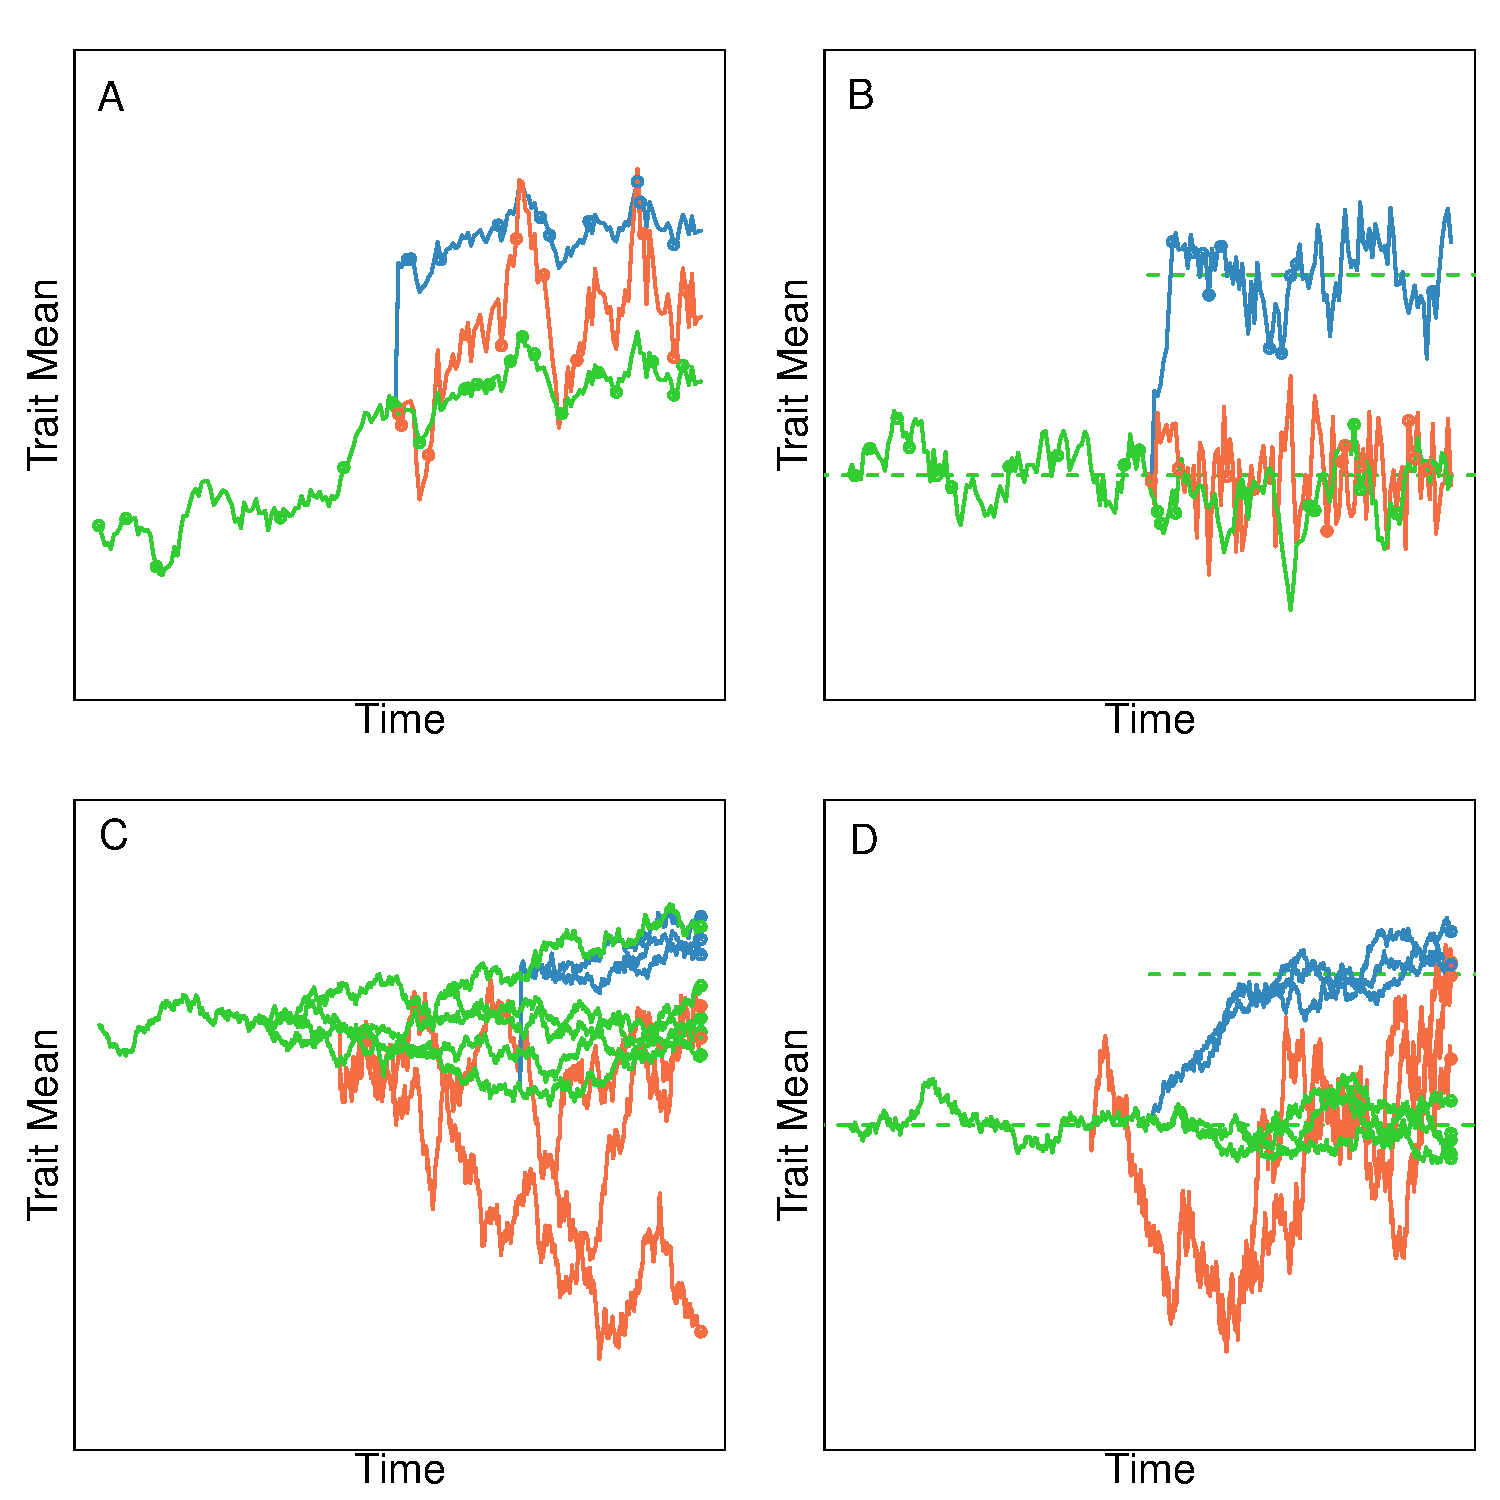
\includegraphics[width=\textwidth]{figs/Pennell_TREE-fig-box1}
\caption[Trait data simulated under alternative models]{Simulated datasets for different models of trait evolution from fossil time--series (A, B) and phylogenetic comparative data (C, D) under Brownian motion models (A, C) and Ornstein--Uhlenbeck models (B, D). Green lines are simulated as constant rate BM and OU processes, with circles indicating sampled data. Blue lines are discontinuous processes in which a burst of evolution occurs in the form of a single displacement (for BM models) or a walk to a new optimum ($\theta_2$) for OU models. However, all other parameters are kept constant. By contrast, red lines are models in which rate parameters ($\sigma^2$ and $\alpha$ for BM and OU models, respectively) shift to higher values and remain constant thereafter, but are not burst--like (no shift in the expected value of the process).  
}
\label{fig:pe-box1}
\end{figure}

BM models predict that divergence can increase without bounds, which is unrealistic under adaptive scenarios of trait evolution or under models of stasis, where traits are expected to evolve around adaptive optima. A simple extension of a BM model is an Ornstein-Uhlenbeck (OU) model of trait evolution. The per unit time change in mean phenotype under this model is:
\begin{equation}
\Delta \bar{z} = -\alpha(\bar{z}-\theta)+\sigma dW
\end{equation}
where $\sigma dW$ is identical to a BM process and contributes stochastically to divergence,  $\theta$ is the optimum trait value, and $\alpha$ is a ``pull'' parameter that governs how strongly the population mean is pulled toward $\theta$. Thus, divergence is a balance between the stochastic diffusion parameter ($\sigma^2$) and the deterministic pull parameter ($\alpha$) toward the optimum value ($\theta$) (Fig. \ref{fig:pe-box1}). As with BM models, discontinuous OU models can allow for shifts in rate parameters ($\alpha$, $\sigma^2$), which has been implemented in a phylogenetic context \citep{Beaulieu2012}. Rapid shifts in optima are more naturally included in OU models via shifts in the $\theta$ parameter, and have been used extensively in phylogenetic comparative methods \citep{Hansen1997, ButlerKing2004, Beaulieu2012}. Population trait means approach a new optimum at a rate proportional to the strength of $\alpha$. Models with alternative patterns of selective regimes can then be compared via model selection techniques to evaluate adaptive hypotheses \citep{ButlerKing2004}. OU models have proven to be very useful for inferring various processes using both phylogenetic comparative \citep{Hansen2008, Mahler2013Science} and paleontological \citep{Hunt2008, Reitan2012} data.


\section{Box 2: An example of how PE can mislead inferences}
From a historical perspective, it is undoubtedly accurate that numerous comparative methods owe their genesis to the framework of PE. However, the temptation to frame these methods as tests of PE is, in our opinion, unwarranted. For example, \citet{Webster2003} developed a method to correlate the total genetic distance between the root and the tip of the tree (hereafter, the path length) with the number of nodes along that path (Fig. \ref{fig:pe-box2}). A significant correlation between path length and the number of nodes rejects constant-rate gradualism in molecular evolution, purportedly in favor of a PE model. This correlation has been repeatedly demonstrated in a variety of datasets in traits ranging from molecular sequences to human languages (\citealt{Webster2003, Pagel2006, Atkinson2008, Lanfear2010}; but see \citealt{Goldie2011}).

\begin{figure}[p]
\centering
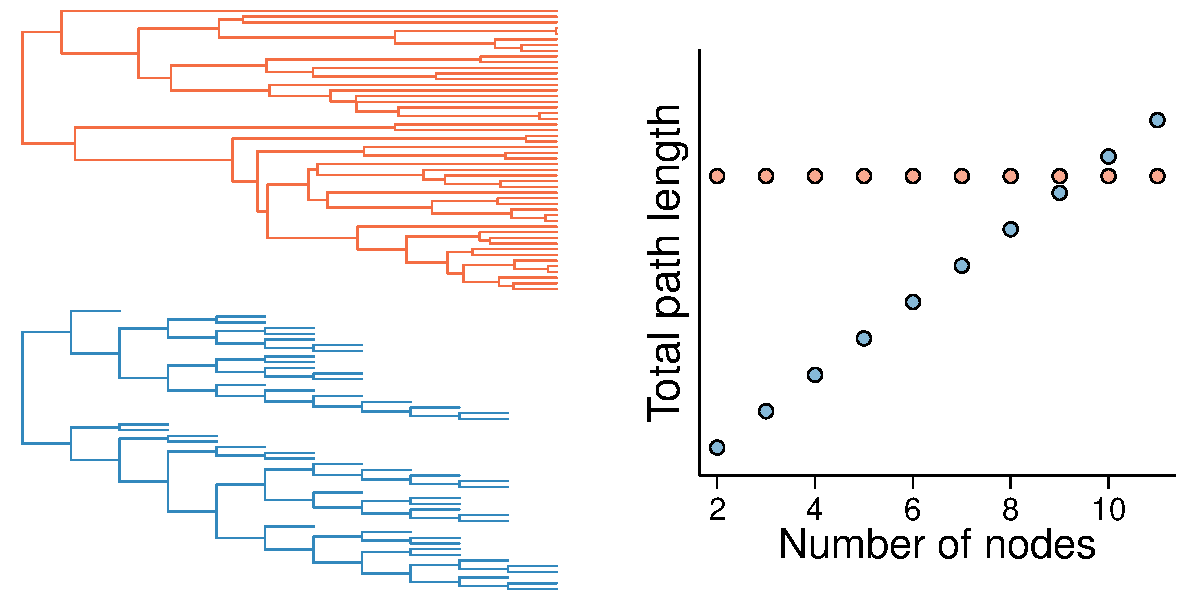
\includegraphics[width=\textwidth]{figs/Pennell_TREE-fig-box2}
\caption[Correlations between evolutionary divergence and speciation rates]{Illustration of a method for correlating evolutionary divergence with speciation. Branch lengths for both phylogenies are in units of evolutionary change. The total path length from the root of the tree to the tips is plotted against the total number of nodes along that path. A positive correlation (blue) is indicative of a relationship between the number of speciation events and evolutionary change, while under constant-rate gradualism no such relationship exists (red). Adapted from \citep{Pagel2006}.}
\label{fig:pe-box2}
\end{figure} 

However, to what extent is there evidence in these cases for PE? We argue: very little. Eldredge and Gould \citep{EldredgeGould1972} hypothesized that allopatric speciation causes pulsed phenotypic divergence. However, the direction of causality can just as easily be reversed. Genetic divergence is expected to promote speciation under many models of speciation \citep{Nosil2012}. Alternatively, divergence and speciation may result indirectly from causal links with a third factor, such as shorter generation times, higher fecundity, or increased genetic variation, to name a few \citep{Goldie2011}. Furthermore, trait evolution need not be pulsed for a positive correlation to exist. This effect was demonstrated by Rabosky \citep{Rabosky2012}, who showed that correlations between path length and speciation are expected whenever trait evolutionary rates are correlated with rates of speciation, even under purely gradual models. 

Finally, trait change may not be correlated with speciation at all, but instead be correlated with extinction rates.  This may occur, for example, if higher evolvability decreases extinction risk \citep{Lanfear2010}. It is certainly a worthwhile avenue of research to establish a correlation between diversification and trait evolutionary rates, but the available tests demonstrate nothing about whether or not trait evolution is pulsed, whether trait change accumulates anagenetically or cladogenetically or the direction of causality. Taking the ``off-the-shelf'' interpretation of these macroevolutionary patterns in the form of PE only obfuscates understanding, and worse, could lead to recapitulating four decades worth of often unproductive and contentious debates. Instead, we argue that we should focus on inferences that may be effectively tested using our available statistical tools. These tools should be integrated with more narrowly--defined theories that are free of the unwanted assumptions of PE.  

\section{Box 3: Modeling species selection and cladogenetic change on phylogenies}

In a ground-breaking paper, Maddison and colleagues \citep{Maddison2007} developed a statistical framework that has opened up investigation into two major components of PE--the influence of traits on diversification \citep[``species selection'', \textit{sensu}][]{CoyneOrr, RaboskyMcCune2010} and cladogenetic character change. The premise of the approach is that instead of specifying a full likelihood of the model, one need only to describe the probabilities of all possible events that could occur in a very short time interval, $\Delta t$, solve a differential equation and then use numerical integration to evaluate the likelihood of the model given the phylogeny and trait data at the tips (see \citealt{Maddison2007}, for full details). The initial model considered by \citet{Maddison2007} was the \textsc{bisse} model in which different states for a single character resulted in different diversification rates.

Consider that lineage diversification can be modeled by a birth-death process \citep{Kendall1948}, in which there is a constant rate of speciation $\lambda$ and extinction $\mu$ across the clade. Lineages with a trait in state $0$ diversify at rates $\lambda_0$ and $\mu_0$ and lineages in state $1$ diversify at rates $\lambda_1$ and $\mu_1$. Transitions (anagenetic evolution) between states $0 \rightarrow 1$ occur at rate $q_{01}$ and transitions from $1 \rightarrow 0$ occur at rate $q_{10}$. The probabilities of all possible events that can occur during $\Delta t$ can be described as a set of differential equations. One can then use the integration machinery, as described in \citet{Maddison2007}, to simultaneously estimate all parameters using either maximum likelihood or Bayesian inference to test for a statistical difference between $\lambda_{0}$ and $\lambda_{1}$ (or between $\mu_0$ and $\mu_1$) in order to infer the strength of species selection.

The \textsc{bisse} model was extended by \citet{MagnusonFord2012} (\textsc{bisse-ness}) to allow for the possibility of character transitions at speciation (cladogenetic change). (An identical model was independently derived by \citealt{Goldberg2012}, and related approaches were also developed by \citealt{Bokma2002, Bokma2008, Bokma2010}.) 

%\begin{figure}[p]
%\centering
%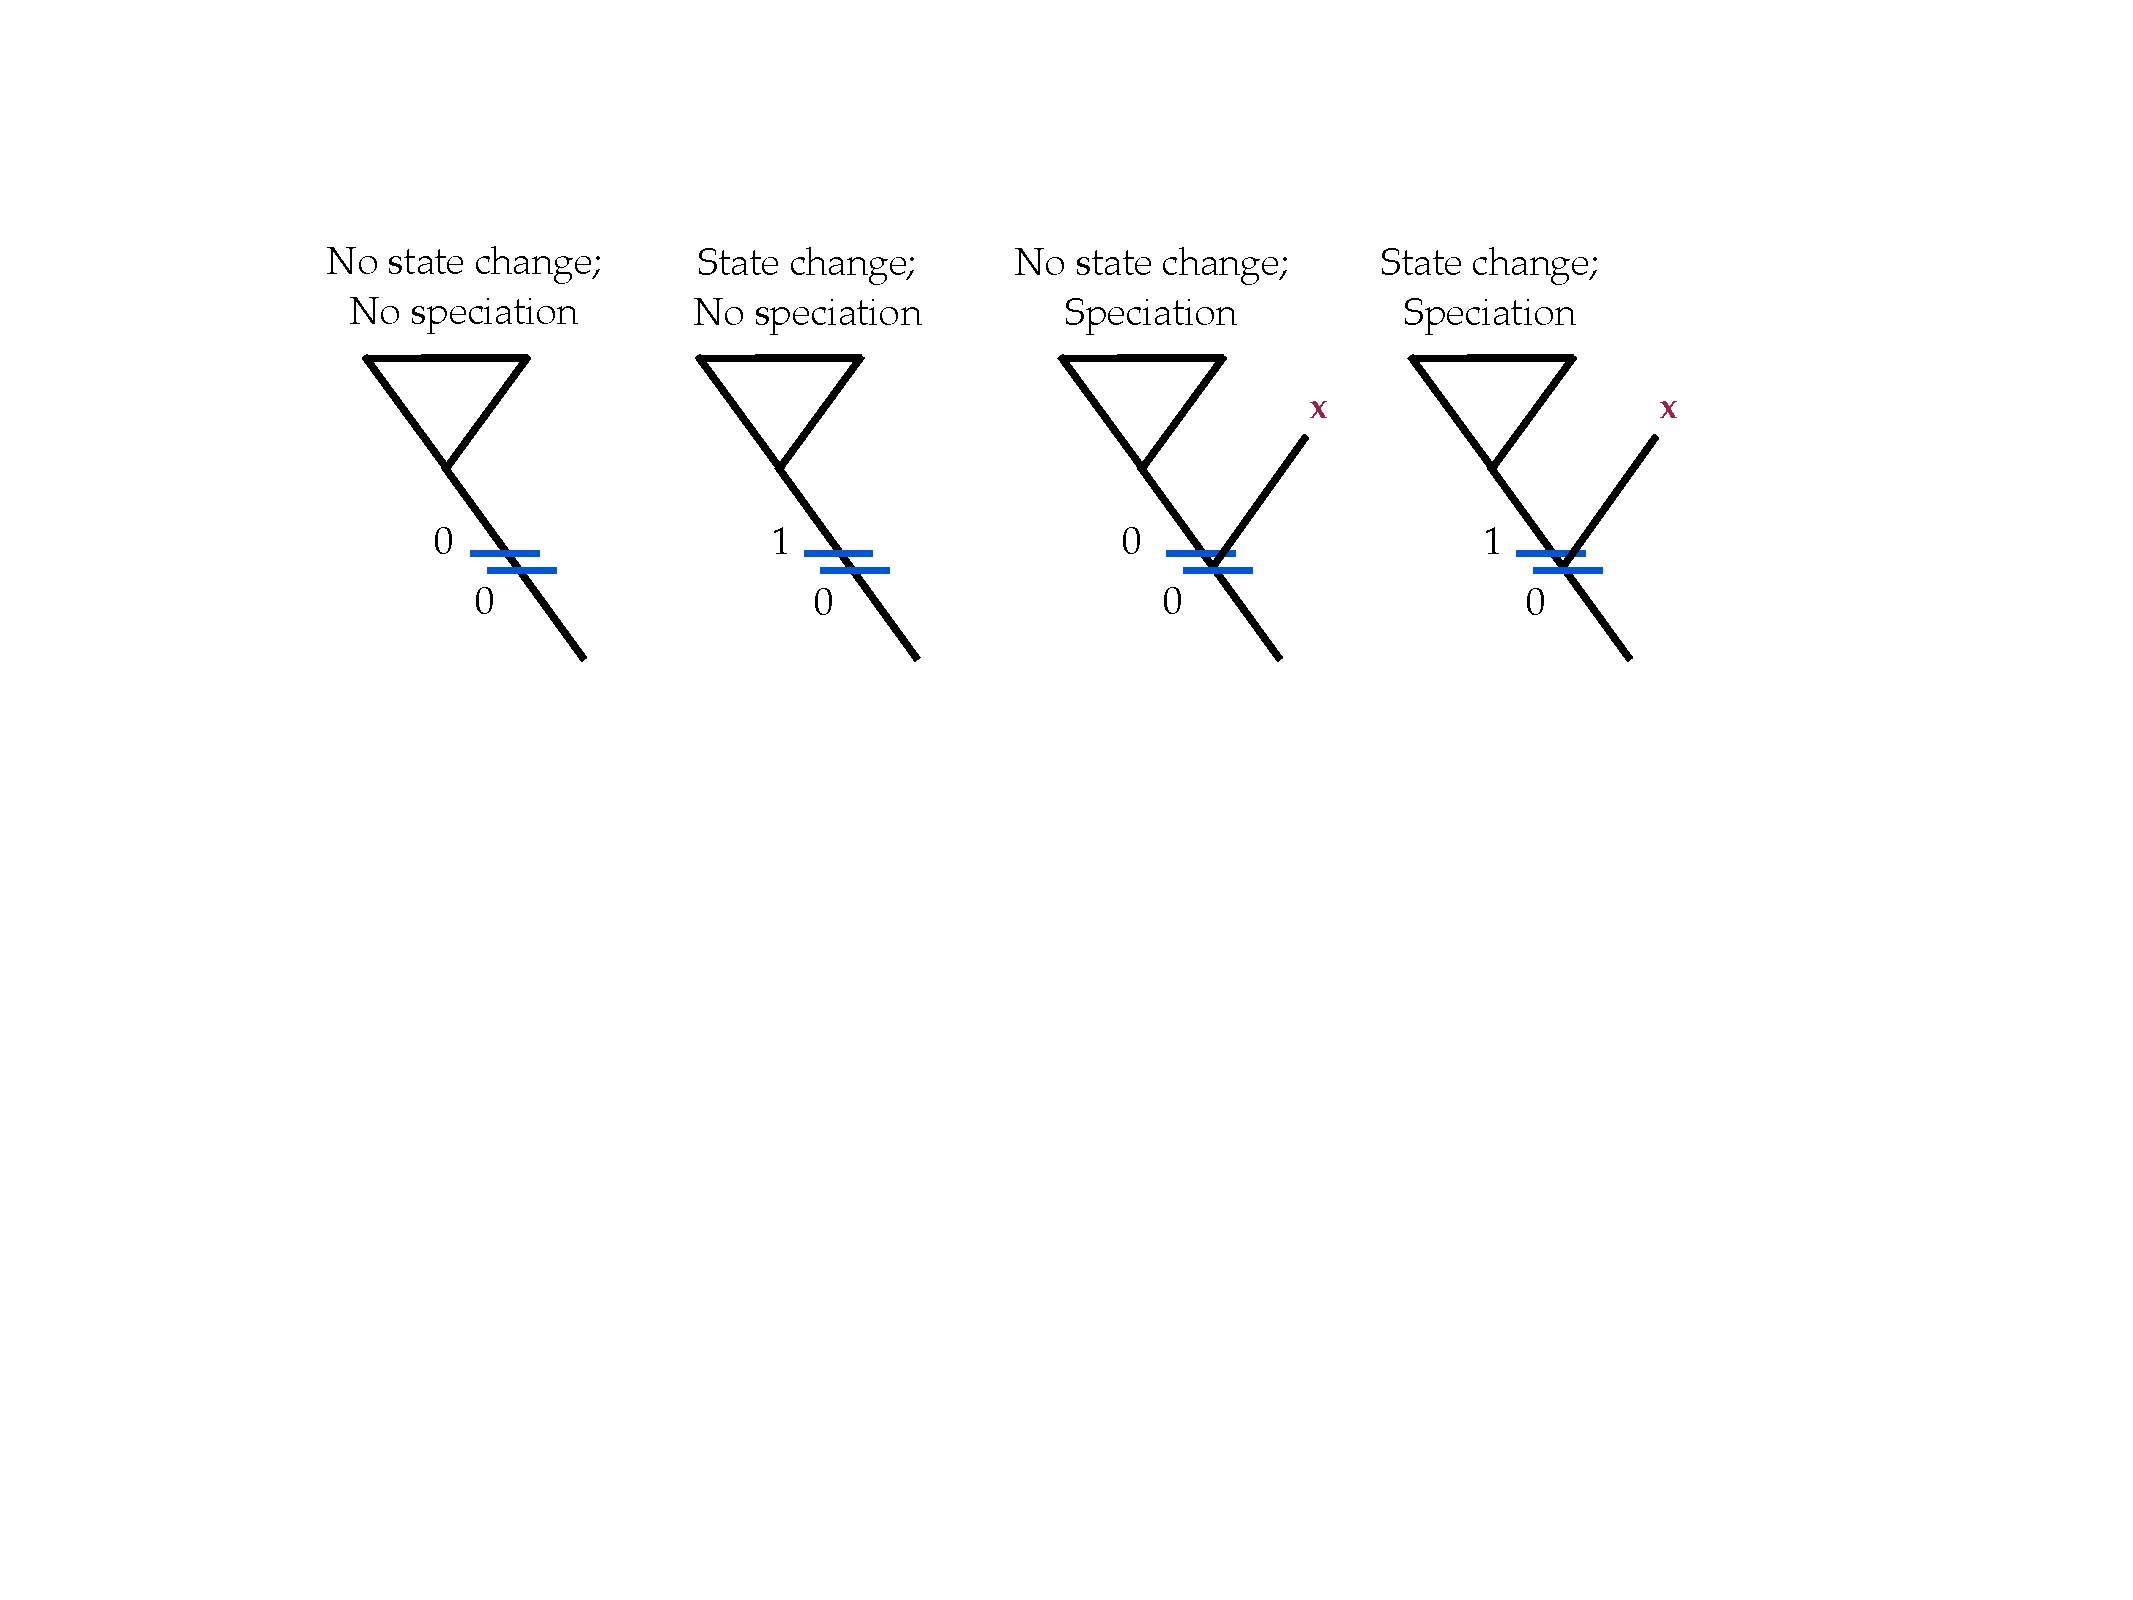
\includegraphics[width=\textwidth]{figs/Pennell_TREE-fig-box3}
%\caption[Illustration of BiSSE model]{A conceptual figure demonstrating how the BiSSE/BiSSE--ness model simultaneously model species selection and trait change. The four trees depict four possible events that could occur during a short time interval ($\Delta t$; the area between the two blue bars) along a given branch: no events happen; the trait changes; speciation occurs; both speciation and trait change occur. (These do not depict all possible scenarios.) If each event can be assigned a probability of occuring over $\Delta t$, one can derive differential equations describing the entire model and use numerical integration to calculate the likelihood of the model given a phylogenetic tree and trait data at the tips. Adapted from \citet{Maddison2007}.}
%\label{fig:pe-box3}
%\end{figure}

In addition to the 6 parameters of the BiSSE model ($\lambda_0, \lambda_1, \mu_0, \mu_1, q_{01}, q_{10}$), their model includes the probabilities of a change occuring at a speciation event ($p_{0c}$ and $p_{1c}$, for the two states, respectively) as well as the probabilities that the character changes are asymmetrical, where the change only occurs in one of the two daughter lineages, $p_{0a}$ and $p_{0b}$ (often referred to as ``budding cladogenesis'' in the paleobiological literature). This allows one to simultaneously evaluate the importance of species selection as well as the relative importance of cladogenetic versus anagenetic change. This model also highlights the general message of our paper; the questions can be evaluated independently of each other if parameter sets are constrained:

\begin{tabular}{ l c r }
  $\lambda_0 = \lambda_1, \mu_0 = \mu_1$ & Estimate cladogenetic and anagenetic rates only \\
  $q_{01}, q_{10} = \text{0}$ & Estimate species selection with only cladogenetic change \\
  $p_{0c}, p_{1c}, p_{0a}, p_{1a} = \text{0}$ & Estimate species selection with only anagenetic change\\
\end{tabular}\\

thus making it an excellent statistical framework, though certainly not the only one, for evaluating the questions associated with PE.


%%% Local Variables:
%%% TeX-master: "thesis"
%%% TeX-PDF-mode: t
%%% End:

\chapter[Software for fitting evolutionary models to phylogenetic data]{Software for fitting evolutionary models to phylogenetic data\footnote{Previously published as: Pennell M.W., Eastman J.M., Slater G.J., Brown J.W., Uyeda J.C., FitzJohn R.G., Alfaro M.E., and Harmon L.J. 2014.
  \textsc{geiger v2.0}: an expanded suite of methods for fitting macroevolutionary
  models to phylogenetic trees. Bioinformatics 15:2216--2218.}} 
\label{chap:geiger}

\section{Summary}
Phylogenetic comparative methods are essential for addressing evolutionary hypotheses with interspecific data. The scale and scope of such data has increased dramatically in the last few years. Many existing approaches are either computationally infeasible or inappropriate for data of this size. To address both of these problems, we present \textsc{geiger v2.0}, a complete overhaul of the popular R package \textsc{geiger} \citep{Harmon2008}. We have re-implemented existing methods with more efficient algorithms and have developed several new approaches for accomodating heterogeneous models and data types.  


\section{Introduction}

In the past few decades, phylogenetic trees have become an key component of evolutionary research. This development has been fueled by the increased availability of robust time-calibrated phylogenies for many groups, in addition to an expanding number of statistical techniques for inferring patterns and processes from comparative data \citep[reviewed in][]{PennellHarmon}. Among the many R packages developed for phylogenetic and comparative data, \textsc{geiger} \citep{Harmon2008} has been a primary utility for making macroevolutionary inferences from phylogenetic trees. 

However, in the six years since the initial release of \textsc{geiger}, the data available for comparative biology have changed substantially. For some groups, we now have phylogenies and corresponding trait data with thousands, and even tens of thousands, of species \citep[e.g.,][]{Jetz2012, Rabosky2012, PyronBurbrink2013, ksi,Zanne}. \textsc{geiger v2.0} is a complete overhaul of the previous release \citep{Harmon2008}, designed to scale up comparative methods to large data sets. To do so,  we have taken two complementary tacks. The first is to improve algorithms and implementations to increase computational efficiency of existing methods. The second is to expand the suite of statistical approaches to allow for heterogeneity in both models and data types across the phylogeny.  

In this chapter, we briefly describe the methods now in \textsc{geiger}, with a particular focus on novel implementations and algorithms. Most of these methods have been previously published elsewhere in some form and we refer readers to the relevant publications for full explanations. For an overview of the main features of the package, see Table \ref{tab:geiger-fxns}.

\begin{table}
\centering
  \begin{tabular}{| p{3.5cm} | p{5.5cm} | p{4cm} |}
    \hline
    Function & Description & Citations \\ \hline
    \texttt{fitContinuous} & Fit continuous trait models with ML & \citet{Felsenstein1973, Hansen1997, Pagel1997, Pagel1999, Blomberg2003, Hunt2006, Harmon2010, FitzJohn2012} \\ \hline
    \texttt{fitDiscrete} & Fit discrete trait models with ML & \citet{Pagel1994, Lewis2001, FitzJohn2009} \\ \hline
    \texttt{rjmcmc.bm} & Fit multi-rate models to continuous traits & \citet{Eastman2011} \\ \hline
    \texttt{rjmcmc.bm} & Fit jump diffusion models to continuous traits & \citet{Eastmanjump} \\ \hline
    \texttt{mecca} & Fit continuous models to unresolved clades with ABC & \citet{Slater2012MECCA} \\ \hline
     \texttt{fitContinuousMCMC} & Fit simple models of continuous trait evolution with MCMC and incorporate fossil data & \citet{Slater2012Fossil} \\ \hline
     \texttt{pp.mcmc} & Posterior predictive simulations to assess model adequacy & \citet{SlaterPennell} \\ \hline
    \texttt{medusa} & Estimate shifts in diversification rates & \citet{Alfaro2009} \\ \hline
     \texttt{congruify.phylo} & Time-scale large phylogenies & \citet{Eastman2013} \\ \hline
  \end{tabular}
\caption[Major features of \textsc{geiger v2.0}]{Major functions of \textsc{geiger v2.0} with description and citations}
\label{tab:geiger-fxns}
\end{table}



\section{Methods}
\subsection{Fitting simple models of character evolution with maximum likelihood}

Fitting and comparing  models of trait evolution can provide insight into many macroevolutionary questions \citep{PennellHarmon}. The two ``workhorse'' functions in \textsc{geiger} for fitting models of trait evolution using maximum likelihood, \texttt{fitContinuous} and \texttt{fitDiscrete}, have both been completely re-implemented. The previous version of \texttt{fitContinuous} calculated the likelihood of a set of continuous characters (e.g., body size) having evolved under a model using a variance-covariance (vcv) matrix approach. This involves inverting the vcv, which is extremely computationally intensive, making the method infeasible for large trees \citep{Hadfield2010, FitzJohn2012, Freckleton2012, Ho2014}. \citet{FitzJohn2012} demonstrated that using a ``pruning''-based algorithm \citep{Felsenstein1973} allows for much more efficient likelihood calculations. This algorithm is used the \textsc{diversitree} package \citep{FitzJohn2012}. (For related algorithms, see \citealt{Freckleton2012}, \citealt{Ho2014}). The approach has now been extended to all the models in \texttt{fitContinuous}. In addition to improving the efficiency of the algorithm, we have improved numerical optimization procedures and implemented a novel method to simultaneuously estimate model parameters and an additional term to account for measurement error.

For discrete character data (for example, the presence or absence of fur), the most commonly used model is the Mk model \citep{Pagel1994, Lewis2001}.  In this model, there are $n$ states $1, 2, ..., n$ and the goal is to estimate rates of
transition among these, where the rate of transition from state $i$ to
state $j \neq i$ is $q_{ij}$.  Considering just one branch in a
phylogeny, let $\vec D$ be the vector of probabilies of the data given
we are in state $i$, that is, the $i$th element of $D$ is the
probability of the data descended from this point in the tree, given
that we are in state $i$; see \citet{Maddison2007} and \citet{FitzJohn2012}
for notation.

In most R-based implementations of Mk, for example, \textsc{ape} \citep{ape}
and previous versions of \textsc{geiger} \citep{Harmon2008} to move from the
tip to the base of a branch, we multiply $\vec D$ by $\mathbf{P}(t)$, the
transition probability matrix with off-diagonal elements that describe
the probability of moving from state $i$ to state $j$ over time $t$
and diagonal elements that describe the probability of not changing
from state $i$.  To compute $\mathbf{P}(t)$, we take the transition rate matrix
$\mathbf{Q}$ composed of $q$ parameters above and compute
$\mathbf{P}(t) = \exp(\mathbf{Q} t)$ where $\exp$ is the matrix
exponential \citep{Sidje-1998-130}.

For \textsc{geiger v2.0} we have sped up these calculations by using an alternative algorithm.
As the number of states gets very large, it is simpler to compute
$\exp(\mathbf{Q}t) \vec D$ directly, rather than in two steps
\citep{Sidje-1998-130}.  This can be done by solving the system of
differential equations
\begin{equation}
\frac{d \vec D}{dt} = \mathbf{Q} \vec D
\end{equation}
subject to the initial condtions at the branch tips.

For small state spaces (a few states to a few tens of states) there
will be no speed differences between these two approaches.  However,
for very large state spaces (hundreds of states) this approach will be
much faster than computing $\exp(\mathbf{Q} t)$ directly.
Importantly, computing $\exp(\mathbf{Q} t)$ grows faster than linearly
in the number of states, while the approach here should grow
approximately linearly.


\subsection{Bayesian methods for fitting models of character evolution}

A major addition to \textsc{geiger} is the implementation of several Bayesian methods for fitting models of trait evolution to comparative data. These include the \textsc{auteur} approach of \citet{Eastman2011}, which uses reversible jump Markov chain Monte Carlo machinery \citep{Green1995} to move across multi-rate  models of various complexity. The implementation of this method in \textsc{geiger v2.0} improves upon the original by allowing model partitions to be constrained \emph{a priori} and alternative models to be compared \citep{Eastmanjump}. Additionally, \textsc{geiger} now includes: a method for fitting models to phylogenies including unresolved clades using Approximate Bayesian Computation \citep[\textsc{mecca};][]{Slater2012MECCA}; a method for including fossil information as priors on node states \citep{Slater2012Fossil}; and a posterior predictive simulation approach for assessing the adequacy of common models of trait evolution \citep{SlaterPennell}. These types of approaches, which allow for greater complexity both in models and data, will be essential to making robust evolutionary inferences from large comparative datasets.  


\subsection{Inferring shifts in the rate of lineage diversification}

\citet{Alfaro2009} developed an approach, \textsc{medusa}, to detect shifts in diversification rates from molecular phylogenies using a stepwise-AIC algorithm. A single-rate birth-death model is fit to the entire tree, then the tree is partitioned into two rate classes, breaking the tree at all possible nodes. The partition which improves the fit of the model is then fixed and the process is repeated, breaking the tree into three partitions, and so on, until a stopping criterion is reached. \textsc{medusa} can be applied to both fully bifurcating and unresolved trees. 

For this release of \textsc{geiger}, the \textsc{medusa} algorithm has been improved in a number of ways. It has been re-coded so that it is now orders of magnitude faster and scales well to large trees; this version of \textsc{medusa} has already been applied to a phylogeny of all 9,993 extant bird species \citep{Jetz2012}. We have also developed tools for summarizing \textsc{medusa} analyses across a distribution of trees, such as from a Bayesian posterior or from non-parametric bootstrapping, so that uncertainty in both topology and branch lengths can be accomodated. we took a simulation based approach. 

The most significant improvement for this version of \textsc{medusa} is in the model selection procedure. As stated above, the \textsc{medusa} algorithm involves comparing the fit of diversification models of varying dimensions (number of parameters). To select an appropriate model, we use Akaike Information Criterion \citep[AIC;][]{Akaike1974}, together with the small-sample bias-correction \citep[AICc;][]{BA2004}:

\begin{equation}
\mathrm{AICc}_{i} = -2 \log (\mathcal{L}_{i}) +
	\frac{2k_{i}n}{n-k_{i}-1}
\end{equation}

where $\mathcal{L}_{i}$ is the maximized joint likelihood of model $i$ with $k_{i}$ estimable (free) parameters, and $n$ data points. Here, $k$ is the number of diversification parameters (net diversification rates, $r_{i} = \lambda_{i} - \mu_{i}$, and extinction fractions, $\epsilon_{i} = \mu_{i}/\lambda_{i}$) plus the number of inferred rate shifts. It is unclear whether the shift locations are indeed `free' parameters of the model as they are not all estimated simultaneously; each additional shift that is introduced reduces the number of possible locations in the next iteration of the algorithm. This is a complex issue and we do not have a strong statistical argument for including them as parameters or not; as such, we have elected to be conservative and penalize adding them as we would any other parameter. For \textsc{medusa}, the sample size $n$ is taken to be the total number of ``observed'' nodes in a tree (internal $+$ pendant). 

However, because \textsc{medusa} considers all possible nested piecewise diversification models, an additional concern is that of multiple testing: as trees grow larger, it becomes increasingly likely that spurious stochastic rate shifts are inferred when no real shifts exist. Indeed, simulations show that the original version of \textsc{medusa} has a high rate of false positives for large phylogenetic trees (more than approximately 50 unresolved tips). We therefore determined an an acceptance threshold (AICc$_t$) through simulation (Figure \ref{fig:medusa-threshold}). 10,000 single-rate birth-death trees were generated for each of a number of resulting extant taxa $N = \lbrace$10, 20, 50, 100, 200, 400, 500, 750, 1000, 1500, 2000, 2500$\rbrace$ using the R package \textsc{treesim} \citep{treesim}. For each simulation we randomly drew diversification parameters where $\lambda \sim \mathcal{U}(0,1]$ and $\mu \sim \mathcal{U}[0, \lambda)$. Each tree was analyzed in \textsc{medusa}, and the difference ($\Delta$AICc) in AICc values between the (true) 0-shift model and best (incorrect) 1-shift model was logged. We then fit a $x$-shifted power function

\begin{equation}
\mathrm{AICc}_{t} = a (N - b)^{c} + x 
\end{equation}

to the 95$^{th}$ percentile $\Delta$AICc values for each tree size (Figure \ref{fig:medusa-threshold}). The best-fitting function had $a =$ -35.94, $b =$ 6.74, $c =$ -0.10, and $x =$ 27.52. If \texttt{partition=NA} (the default argument in the \texttt{medusa} function), the AICc$_{t}$ is automatically calculated for the specified tree from this best-fitting function. For trees of 20 or fewer taxa, AICc$_{t}$ is set to 0.

\begin{figure}[p]
 \centering
  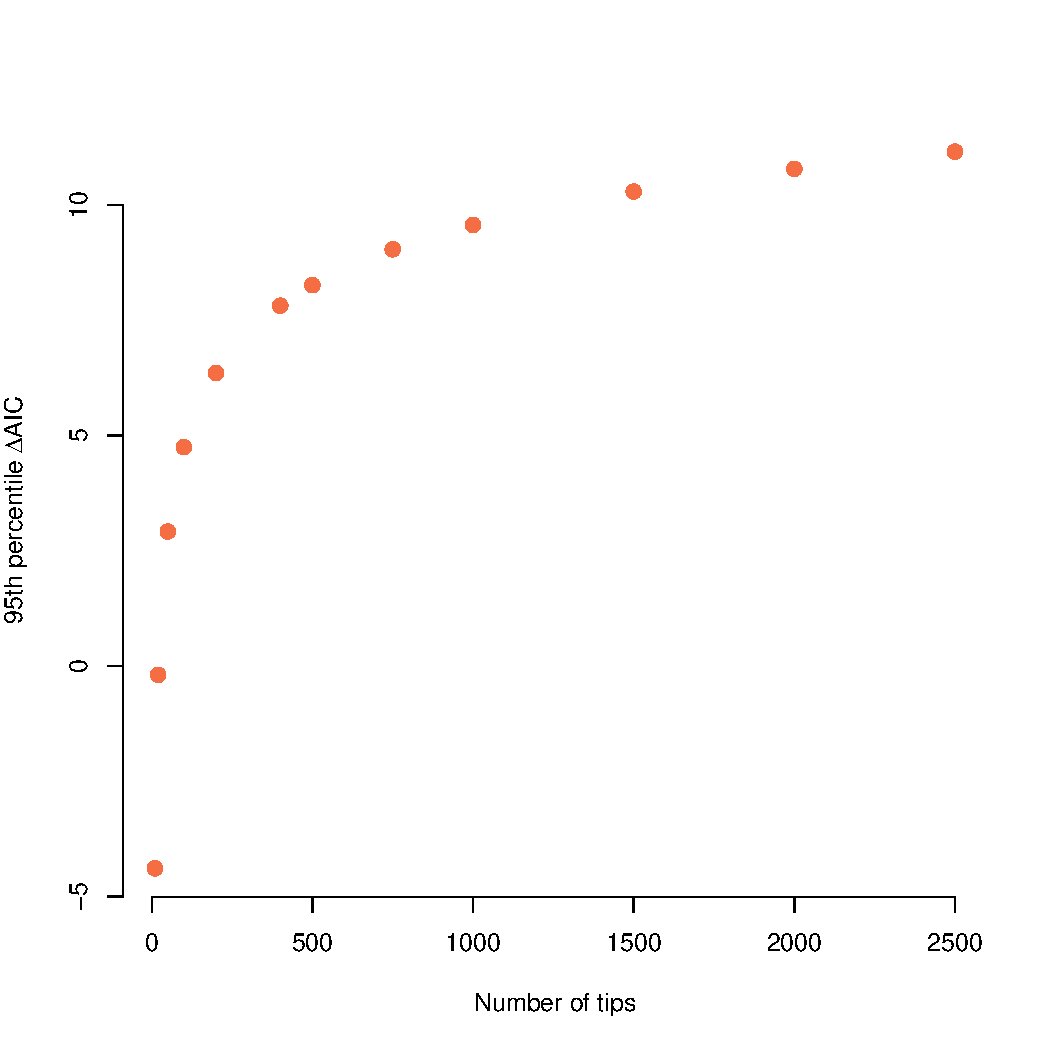
\includegraphics[width=\textwidth]{figs/BD_percentiles}
  \caption[Setting the \textsc{medusa} threshold via simulation]{The 95$^{th}$ percentile values for the difference in AICc scores ($\Delta$AICc) between the (incorrect) 1-shift model and the (true) 0-shift model plotted against simulated tree size. We fit a $x$-shifted power function to these points to estimate a AICc$_{t}$ with a Type-1 error rate of 0.05 for a given tree with $N$ tips.}
  \label{fig:medusa-threshold}
\end{figure}


\section{Concluding remarks}

In this note we provide a broad overview of the methods now available in \textsc{geiger}. We have not discussed some methods implemented in \textsc{geiger} \citep[e.g., `Congruification' for time-scaling large trees;][]{Eastman2013} and many of the nuances of the methods described here have been left out. We refer readers to associated publications and the package documentation for more information.

It is an exciting time for macroevolutionary research. We now have access to data sets of unparalleled size and a wide variety of new statistical approaches with which to analyze them. We hope that the software presented here will help researchers address some fundamental and long-standing questions in macroevolution. 

\chapter[Y fuse? Using phylogenetic comparative and population genetic models to understand sex chromosome fusions]{Y fuse? Using phylogenetic comparative and population genetic models to understand sex chromosome fusions \footnote{Submitted as: Pennell, M.W., M. Kirkpatrick, S.P. Otto, J.C. Vamosi, C.L. Peichel, N. Valenzuela, and J. Kitano. Y fuse? Sex chromosome fusions in fishes and reptiles}}
\label{chap:sexchrom}

\section{Summary}

The evolution of chromosome number plays an important role in divergent adaptation and speciation. Chromosomal fusion is a common mechanism of karyotypic evolution, but there is little understanding of the evolutionary forces that have driven chromosomal fusions. Because sex chromosomes (X and Y in male heterogametic systems, Z and W in female heterogametic systems) differ in their selective, mutational, and demographic environments, those differences provide a unique opportunity to dissect the evolutionary forces that drive chromosomal fusions. We estimate the rate at which fusions between sex chromosomes and autosomes establish across the phylogenies of both fishes and squamate reptiles. Both the incidence among extant species and the establishment rate of Y-autosome fusions is much higher than for X-autosome, Z-autosome, or W-autosome fusions. Using population genetic models, we show that this pattern cannot be reconciled with many standard explanations for the spread of fusions. In particular, direct selection acting on fusions or sexually antagonistic selection cannot, on their own, account for the predominance of Y fusions. We identify three plausible explanations for the excess of Y-autosome fusions: (i) fusions are deleterious, and the mutation rate is male-biased or the reproductive sex ratio is female-biased, (ii) fusions capture loci under sexually antagonistic selection, and the mutation rate is male-biased or the reproductive sex ratio is female-biased, and (iii) meiotic drive acts against fusions in females. These results may shed light on the processes that drive structural changes throughout the genome.

\section{Introduction}

The number of chromosomes is one of the most fundamental features of a eukaryotic genome. Chromosome number often varies within species or between closely related species, and such variation can contribute to divergent adaptation and speciation \citep{White1973, King1993}. Although genetic drift, selection for reduced recombination, and meiotic drive are hypothesized to fix chromosomal fusions \citep{Nachman1995, Guerrero2014}, we have an incomplete understanding of the evolutionary forces that allow fusions and fissions to become established.

Sex chromosomes offer a unique opportunity to dissect these forces. The X and Y chromosomes of male-heterogametic species (as in mammals) and the Z and W chromosomes of female-heterogametic species (as in birds) differ in many aspects of their evolutionary environments, particularly with respect to hemizygosity (i.e., XX and ZZ individuals are common, but not YY and WW). While Y and W chromosomes are often thought to be evolutionarily similar, they differ in the amount of time spent in males and females: Y chromosomes spend 100\% of their evolutionary history in males, while W chromosomes spend none. X and Z chromosomes also differ: X chromosomes spend 1/3 of their evolutionary history in males, while Z chromosomes spend 2/3 of their history in males. Consequently, the four types of sex chromosomes vary in how selection acts on them, in their effective population sizes, in their mutation rates, and in the relative importance of meiotic drive \citep{Ellegren2011, Bachtrog2011, Perrinbook}. All of these factors could play a role in the evolution of chromosomal rearrangements, and so differences in rates of rearrangement among sex chromosomes offer clues to what evolutionary conditions favor changes to genome structure.

Structurally, sex chromosomes are the most rapidly evolving parts of the genome in many groups of animals \citep{White1973, Bull1983, Ezaz2006,Perrinbook} In some taxa, such as fishes and squamate reptiles, closely related species (and even populations within a species) differ in how sex is determined \citep{Ezaz2006, Bachtrog2014}. Further, a large number of fusions between sex chromosomes and autosomes have been discovered \citep{White1973, ToS}. Thus there are many phylogenetically independent events, providing the opportunity to test whether fusions involving the four different types of sex chromosomes are equally likely to occur and/or establish within a species.
 
A fusion between a sex chromosome and an autosome can usually be detected because it creates an odd number of chromosomes in one sex \citep[Fig. \ref{fig:fuse-diag};][]{White1973, Ohno1967}. With XY sex determination, a Y-autosome fusion creates an X1X2Y system, with the unfused homologue segregating as a neo-X chromosome. Likewise, X-autosome fusions generate XY1Y2 systems, Z-autosome fusions generate ZW1W2 systems, and W-autosome fusions generate Z1Z2W systems. These neo-sex chromosome systems can often be identified by light microscopy, without molecular cloning or linkage mapping. This has enabled cytogenetic studies to identify many species with sex chromosome-autosome fusions \citep{White1973, Ezaz2009, Kitano2012, Yoshida2012, Maddison2013}. These data have yet to be used to estimate rates of different types of sex-autosome fusions.

\begin{figure}
\centering
\includegraphics[width=\textwidth]{figs/Fuse-Fig1}
\caption[Schematic of sex chromosome fusions]{Sex chromosome-autosome fusions create multiple sex chromosome systems. (A) In XY systems, X-autosome and Y-autosome fusions make XY1Y2 and X1X2Y systems, respectively. (B) In ZW systems, Z-autosome and W-autosome fusions make ZW1W2 and Z1Z2W systems, respectively.}
\label{fig:fuse-diag}
\end{figure}

Three main evolutionary forces have been thought to be important to the establishment of fusions. The first is direct selection. While chromosome rearrangements are often considered deleterious \citep{King1993, Gardner2012}, chromosomal translocations may alter the expression of genes near the breakpoint \citep{Ohno1967, Dobigny2004}, which may sometimes be beneficial \citep{PerezOrtin2002, Chang2013}. A second mechanism that has been proposed to establish fusions is sexually antagonistic selection at an autosomal locus \citep{Charlesworth1982}. A fusion with a sex chromosome can cause an allele that is beneficial in one sex to spend more than half of its evolutionary life in that sex. Meiotic drive is a third force. During female meiosis in animals, one of the products of meiosis goes into the egg, while the others are discarded in the polar bodies. In some species, female meiotic drive preferentially transmits fused chromosomes to eggs, while unfused chromosomes go into polar bodies \citep{Pardo2001a, Pardo2001b}. This drive favors X-autosome fusions because they experience female meiosis in two of every three generations. In other species, female meiotic drive preferentially transmits fused chromosomes, which should select against X-autosome fusions \citep{Yoshida2012}. While these evolutionary forces are known to affect the spread of sex chromosome-autosome fusions, previous work has not examined the relative rates at which fusions with different types of sex chromosomes establish within a population.
 
We begin this study by analyzing a large new data set that includes information on the sex determination system and karyotypes across the tree of life \citep{ToS}. We focus on fishes and squamate reptiles because these taxa include many independent origins of XY and ZW systems \citep{Ezaz2009, Kitano2012}, allowing us to assess differences in the rates of fusions. We find that Y-autosome fusions fix at a much higher rate than any of the other three types of sex chromosome-autosome fusions. This then motivates us to develop an integrated body of analytic models that predict the relative fixation rates for the different types of fusions. The models incorporate a large number of potentially important factors: deleterious and beneficial effects of fusions, sexually antagonistic selection, female meiotic drive, genetic drift, sex-biased mutation rates, and biased sex ratios. We find that several of the data cannot be explained by some of the most frequently-discussed hypotheses. There are, however, several combinations of forces that are able account for the observed patterns of sex chromosomes fusions, as we highlight.

\section{Analysis of patterns of sex chromosome-autosome fusions in vertebrates}

We compiled lists of species with multiple sex chromosome systems (X1X2Y, XY1Y2, ZW1W2, and Z1Z2W systems) from the Tree of Sex database \citep{ToS}. Although X1X2Y systems (or ZW1W2 systems) can also arise from species with XO (or ZO) systems through a reciprocal translocation between an X (or a Z) and an autosome \citep{White1973, Kitano2012}, XO or ZO systems are rare in vertebrates \citep{ToS} (Table \ref{tab:fusions}). In addition, although fission of sex chromosomes can also create multiple sex chromosome systems \citep{White1973, Kitano2012}, such fissions are also rare in vertebrates \citep{Ohno1967, Kitano2012, Yoshida2012}. Therefore, we considered that most multiple sex chromosome systems are derived from sex chromosome-autosome fusions in vertebrates. We address two questions with our empirical analyses. First, do Y-A (W-A) fusions occur at different rates than X-A (Z-A) fusions? Second, are there differences in rates of fusion between male and female heterogametic lineages? For both questions, we first simply tabulated the numbers in the database and computed Fisher's exact test. This ignores phylogenetic non-independence but allowed us to use all of the available data. 

We begin by analyzing the patterns of chromosome fusions in vertebrates, based on our recent compilation of sex chromosome data \citep{ToS}. Examining the raw counts (Table 1), two interesting patterns emerge. First, there are more species with Y-A fusions (X1X2Y karyotype, 101 species) than with X-A fusions (XY1Y2 karyotype, 27 species). (We use, e.g., Y-A fusion as shorthand for a fusion between a Y chromosome and an autosome.) The pattern is particularly strong in both fishes and squamate reptiles, while the numbers are more nearly equal in mammals (Table \ref{tab:fusions}). Such counts, however, do not account for the phylogenetic relatedness among many of the species. Second, sex chromosomes in XY lineages are more often fused than those in ZW lineages (Table 1). In fishes, 41.3\% (45/109) of XY species have fused sex chromosomes, whereas only 5.3\% (2/38) of ZW species do (Fisher's exact test $p < 0.001$). In reptiles, 33\% (40/120) of XY species have fusions, whereas only 2.5\% of species (6/240) of ZW species do (Fisher's exact test $p < \text{0.001}$).

\begin{table}
\centering
\begin{tabular}{|p{.15\textwidth} |p{.1\textwidth} |p{.1\textwidth}|p{.1\textwidth}|p{.1\textwidth}|p{.1\textwidth}|p{.1\textwidth} |}
\hline
Taxa & Y-A (X1X2Y) & X-A (XY1Y2) & W-A (Z1Z2W) & Z-A (ZW1W2) & XY systems & ZW systems \\ \hline
Fish & 42 & 3 & 0 & 2 & 109 & 38 \\\hline
Amphibians & 1 & 0 & 0 & 0 & 29 & 16 \\\hline
Reptiles & 40 & 0 & 2 & 4 & 120 & 240 \\\hline
Birds & - & - & 2 & 4 & 0 & 192\\\hline
Mammals & 18 & 24 & - & - & 467 & 0\\\hline
\end{tabular}
\caption[Records of sex chromosome-autosome fusions in vertebrates]{Observed number of species with multiple sex chromosome systems in vertebrates. Only X1X2Y, XY1Y2, Z1Z2W, and ZW1W2 systems are counted here.}
\label{tab:fusions}
\end{table}
   

To gain a better estimate of the rates at which fusions establish with different chromosomes, we fit phylogenetic models to the fusion data. We first matched sex chromosome systems from the fish dataset to a recent time-calibrated phylogeny of teleosts \citep{Rabosky2013}, containing 7811 species (we note that a small number of species were removed from the published phylogeny due to errors discovered after publication; M. Alfaro, personal communication). We matched the data of sex chromosome systems from squamates to the squamate phylogeny \citep{Pyron2013, PyronBurbrink2013} using genetic data from 4161 species. In order to maximize overlap between the trait data and the species, we used an approximate matching algorithm for unmatched species: 1) retain all species that occur in both the tree and the dataset; 2) replace an unmatched species in the tree with a randomly selected unmatched species in the dataset from the same genus as long as this did not result in more than two representatives from the genus (this assumes monophyly of genera but avoids determining node order for nodes not in the original trees). We then pruned down the phylogeny down to those tips with data assignments.This resulted in phylogenetic comparative datasets containing 163 species of fish \ref{fig:phylo-fish} and 261 squamate \ref{fig:phylo-squa} species.

\begin{figure}
\centering
\includegraphics[width=\textwidth]{figs/Fuse-Fig2}
\caption[Phylogenetic distribution of sex chromosome fusions in fish]{Sex chromosome fusions (outer circle) and sexual determination system (inner circle) mapped onto the phylogenetic trees of fish. The vast majority of fusions occur in XY systems (aqua) and involve Y-A fusions (brown).}
\label{fig:phylo-fish}
\end{figure}

\begin{figure}
\centering
\includegraphics[width=\textwidth]{figs/Fuse-Fig3}
\caption[Phylogenetic distribution of sex chromosome fusions in squamates]{Sex chromosome fusions (outer circle) and sexual determination system (inner circle) mapped onto the phylogenetic trees of squamate reptiles. The vast majority of fusions occur in XY systems (aqua) and involve Y-A fusions (brown).}
\label{fig:phylo-squa}
\end{figure}



We conducted two separate types of analyses on both groups. First, we examined differences between XY and ZW systems; here, we treat X-autosome and Y-autosome fusions as equivalent (and likewise, Z-autosome and W-autosome fusions). Results from this first analysis are presented in the main text. Second, we investigated autosomal fusion rates for all types of sex chromosomes individually (i.e., Y-, X-, W-, and Z-autosome fusions). While the second analysis provides more detailed resolution, some of the states are rarely observed (and in some cases, not at all). All analyses were performed using the R package \textsc{diversitree} \citep{FitzJohn2012}, and code to reproduce all results can be found at \texttt{https://github.com/mwpennell/fuse/analysis}. 

\subsection{Fusion rates in XY vs. ZW systems}

Using a Markov model \citep{Pagel1994}, we considered transitions among the following states:
\begin{itemize}
\item $XY$: Male heterogametic unfused
\item $XY_F$: Male heterogametic fused (XXY or XYY)
\item $ZW$: Female heterogametic unfused
\item $ZW_F$: Female heterogametic fused (ZZW or ZWW)
\end{itemize}
allowing transitions between all states with $q_{A.B}$ representing the transition rate between states $A$ and $B$. We then used likelihood ratio tests to restrict the model in order to improve our ability to estimate the parameters of interest. 

We first imposed the biologically reasonable constraint that prior to becoming $XY_F$ (or $ZW_F$), a lineage must first be $XY$ (or $ZW$); e.g., the transition rate from female heterogametic unfused to male heterogametic fused $q_{ZW.XY_F}$ would be zero. These restrictions did not lead to a significant decline in likelihood for either squamates or fish and was accepted. Next, we proposed a model in which the rate of switching the heterogametic sex, going from a XY to a ZW system and \emph{vice versa}, did not depend on whether the lineage contained a fused sex chromosome or not (e.g., $q_{XY_F.ZW} = q_{XY.ZW}$). In both fish and squamtes, this restriction was acceptable.

In the next step, we proposed a model in which the rate of chromosomal fission, going from a fused sex chromosome system to an unfused system of the same type, was the same for XY and ZW systems. In fish, a likelihood ratio test favored the more restricted model, whereas in squamates, the more general model (where $q_{XY_F.XY} \neq q_{ZW_F.ZW}$) was favored ($p=\text{0.012}$). The support for the more general model in squamates stems from the scarcity of ZW fusions in the data; there is little information to reliably estimate the transition rate from fused female heterogametic to unfused female heterogametic ($q_{ZW_F.ZW}$) using maximum likelihood (see below). We therefore took slightly different approaches when analyzing the two clades.

For fish, we compared the resulting model ($q_{XY_F.XY} = q_{ZW_F.ZW}, q_{ZW.XY_F}=q_{XY.ZW_F}=\text{0}, q_{XY_F.ZW}=q_{XY_Z.ZW}, q_{ZW_F.XY}=q_{ZW.XY}$) to an even more reduced model in which the XY and ZW fusion rates were set to be equal ($q_{XY.XY_F}=q_{ZW.ZW_F}$). We found the rate difference to be highly significant ($p=\text{0.014}$) using a likelihood ratio test. To better accomodate uncertainty in the estimate, we ran a Bayesian analysis. We set broad exponential priors on all parameters ($\lambda=20$) and sampled 50,000 generations of the MCMC, discarding the first 10,000 as burnin. This also supported our conclusion that XY fusions occur at a higher rate than ZW fusions (98.6\% of the posterior probability supported this and the 95\% credibility interval for the difference in rates did not overlap with zero; Fig. \ref{fig:pp-fuse-final}).

\begin{figure}
\centering
\includegraphics[width=\textwidth]{figs/fusion-rates-xyzw}
\caption[Fusion rate difference between XY and ZW systems]{Posterior probability density of the difference in fixation rates of fusions between autosomes and sex chromosomes (rates in XY species minus in ZW species). The plot illustrates the difference in fusion rates over the last 40,000 steps of an MCMC chain, with the 95\% credibility intervals shown by the horizontal bars below the figure.}
\label{fig:pp-fuse-final}
\end{figure}

For the squamate data, we took two approaches. First, we assumed that the `equal fission rates model' was indeed reasonable and performed the same analysis as in fish. Using a likelihood ratio test, the difference in fusion rates for XY and ZW was found to be highly significant ($p=\text{0.003}$). The same was true for the Bayesian analysis (99.9\% of the posterior probability distribution supported this conclusion; Fig. \ref{fig:pp-fuse-final}). Second, we used a Bayesian MCMC to fit a model in which the fission rate $q_{ZW_F.ZW}$ was estimated independently of $q_{XY_F.XY}$. For this model the support for the difference between XY and ZW fusion rates was not as strong (92.0\% of the posterior probability supported $q_{XY.XY_F} > q_{ZW.ZW_F}$; Figure \ref{fig:squa-dif}).

\begin{figure}[p]
\centering
\includegraphics[scale=1.25]{figs/karyotype-fusion-squa-6par}
\caption[Fusion rate difference between XY and ZW systems (alternate model)]{Posterior estimate of the rate difference between XY and ZW fusions ($q_{XY.XY_F} - q_{ZW.ZW_F}$) in squamate reptiles when we allow the fission rates $q_{XY_F.XY}$ and $q_{ZW_F.ZW}$ to differ.}
\label{fig:squa-dif}
\end{figure}

As mentioned above, the squamate data contain very little information about fission rates, especially from $ZW_F$ to $ZW$. The likelihood approach has difficulty distinguishing between two explanations for the lack of fused ZW chromosomes: rare ZW fusions or common ZW fissions. Nevertheless, there is a strong signal that ZW fusions should be less common, which we confirmed by considering residency times $t_R$. For XY fusions,
\begin{equation}
t_{R,XY_F} = \frac{q_{XY.XY_F}}{q_{XY.XY_F} + q_{XY_F.XY}}
\end{equation}
and for ZW fusions
\begin{equation}
t_{R,ZW_F} = \frac{q_{ZW.ZW_F}}{q_{ZW.ZW_F} + q_{ZW_F.ZW}}
\end{equation}
Using a Bayesian analysis, we found very strong support for the residency time being greater for XY fusions than ZW fusions (99.8\% of the posterior probability supported $t_{R,XY_F} > t_{R,ZW_F}$; Figure \ref{fig:squa-resid}). In the absence of direct information about fission rates for fused ZW chromosomes, we conclude that the data is more parsimoniously explained by rare ZW fusions, while acknowledging that rapid ZW fission rates may also explain the data for squamates.

\begin{figure}[p]
\centering
\includegraphics[scale=1.1]{figs/karyotype-residency-squa-6par}
\caption[Fusion residency time in squamates]{Posterior estimate of the difference in residency time between XY and ZW fusions (i.e., $t_{R,XY_F} - t_{R,ZW_F}$) in squamate reptiles.}
\label{fig:squa-resid}
\end{figure}


\subsection{Comparing fusion rates between chromosomes} 

Rather than classifying the states as male/female heterogametic unfused/fused, we separated out the different types of fusions (e.g., classifying X-autosome [XA] and Y-autosome [YA] fusions as different states). This allowed us to assess whether the patterns we observed were driven by an overabundance of autosomal fusions with the Y chromosome. After matching the data to the tree, we did not have any records of WA fusions in fish while in squamates, XA fusions were absent. We thus considered models with only three fused states (for fish: XA, YA, and ZA; for squamates: YA, WA, and ZA)

For both the fish and the squamates, we again restricted the model via a nested series of likelihood ratio tests. For both clades, we found it to be statistically justifiable to assume that: a) transitions from one fused state directly to another fused state were impossible; b) prior to becoming fused, a lineage had to be in the corresponding unfused state; and c) fission rates were constrained to be equal. This allowed us to reliably evaluate whether the fusion rates differed by chromosome.

For the fish, using likelihood ratio tests, we found YA fusions to be significantly higher than XA fusions ($p=\text{0.016}$) and ZA fusions ($p=\text{0.035}$), but that XA and ZA fusion rates were not significantly different ($p=\text{0.658}$). Again, WA fusions did not exist in the fish analysis so we could not compare them to other classes. We then performed a Bayesian MCMC analysis to gain a better estimate of the relevant parameters. For the purposes of this analysis, we fixed XA and ZA fusions to occur at the same rate and then compared this rate to that for YA fusion. We found that YA fusions occur at a much higher rate than XA/ZA fusions (Figure \ref{fig:fish-ind}; 99.5\% of the posterior distribution supported this conclusion).

\begin{figure}[p]
\centering
\includegraphics[scale=1.25]{figs/chromosome-fusion-fish}
\caption[Comparison of Y-autosome and X-/Z-autosome fusion rates (fish)] {Posterior estimate of the rate difference between YA and XA/ZA fusions in fish. When the estimate is greater than zero, this means that the YA fusion rates are higher than those of the other chromosomes}
\label{fig:fish-ind}
\end{figure}

For the squamate analysis, YA fusions also occured at a higher rate than WA fusions ($p<\text{0.001}$) and ZA fusions ($p<\text{0.001}$). WA and ZA fusions rates were not significantly different from one another ($p\approx \text{1}$). As with the fish, for the Bayesian analysis we set WA and ZA fusion rates to be equal and estimated the difference between YA fusions and other type of fusions. 99.9\% of the posterior probability distribution supported YA fusions occuring at a higher rate than fusions on other chromosomes (Figure \ref{fig:squa-ind}). 

Taken together, these results strongly suggest that the difference between XY and ZW fusion rates is driven almost entirely by the very high rates of autosomal fusions involving the Y chromosome relative to the other sex chromosomes.

\begin{figure}[p]
\centering
\includegraphics[scale=1.25]{figs/chromosome-fusion-squa}
\caption[Comparison of Y-autosome and W-/Z-autosome fusion rates (squamates)]{Posterior estimate of the rate difference between YA and WA/ZA fusions in squamate reptiles. When the estimate is greater than zero, this means that the YA fusion rates are higher than those of the other chromosomes}
\label{fig:squa-ind}
\end{figure}

\section{Theoretical analysis}

To evaluate the plausibility of various mechanisms to explain the excess of fusions involving Y chromosomes, we modeled the rate of establishment of different sex chromosome-autosome fusions under various evolutionary scenarios. The core results are derived in \spacedsmallcaps{Appendix a}, where we approximate the rate, $R_C$, at which a given type of chromosome fusion $(C = X, Y, Z, \text{or} W)$ establishes within a population, accounting for both the rates that different types of fusions arise in a population and the probabilities that they fix.

To facilitate comparison to the data, we focus on the establishment rates for Y-A, Z-A, and W-A fusions relative to the rate of X-A fusions. We begin by studying the neutral case, where selection is absent. We allow, however, for sex-biased mutation rates and sex-biased sex ratios (see \spacedsmallcaps{Appendix a} for definitions). We then ask how these neutral results are altered by the three main evolutionary forces thought to impact the rate of fusions: direct selection acting on the fusion, meiotic drive, and sexually antagonistic selection.

\subsubsection{Neutral case}

We first consider the case without any selection or drive in the model. The overall establishment rates for fusions are given by the mutation rates generating each type of fusion (\spacedsmallcaps{Appendix a}, Equation A.6). Interestingly, the sex ratio does not enter into these results. Among newborns, each copy of a particular sex chromosome has an equal chance of being the progenitor of the entire population of that sex chromosome at some distant point in the future, regardless of subsequent changes in the survival and reproductive success of males versus females. 

Sex-biased mutation would alter the relative frequencies that different types of neutral fusions become fixed. Evidence suggests that the sexes differ substantially in the rate at which fusions arise. Data from humans indicates that balanced translocations are the most likely source of new fusions \citep{Schubert2011}, and these seem to be predominantly paternal in origin \citep{Batista1993, Sartorelli2001, Wyrobek2006, Thomas2010, Grossmann2010, Schubert2011}. If mutation is male-biased but does not depend on the type of chromosome (that is, the X and Y chromosomes in a male are equally likely to fuse), then Y-A fusions will fix most frequently (see eq. A7). In this case, however, Z-A fusions would be almost as common as Y-A fusions (at least 2/3 as common, see eq. A7 and Fig. 5B black curves), which is not seen in the data (Figs. \ref{fig:phylo-fish} and \ref{fig:phylo-squa}). Thus the hypothesis that sex-autosome fusions are selectively neutral does not appear consistent with the data.

\subsubsection{Direct fitness effects}

Direct fitness effects: We next ask how relative establishment rates depend on the direct fitness effects of a fusion (\spacedsmallcaps{Appendix a}). Assuming that the fusion has an additive effect on fitness and that all else is equal (unbiased reproductive sex ratios and mutation rates, and equal fitness effects for all types of fusions), the establishment rate is equal for X-A and Z-A fusions and for Y-A and W-A fusions. Fusions involving the Y or W are a factor 
\[\frac{1}{3}(1 + e^{-2N_s} + e^{-N_s})\]
more common, where N is the number of reproductive adults and s is the fitness effect of the fusion. Thus, deleterious fusions ($s<\text{0}$) are much more likely to involve the Y or W chromosome, because of the smaller population size of these chromosomes. Conversely, beneficial fusions are more likely to involve X or Z chromosomes because they are more numerous and so more often the targets of beneficial fusions. 

Direct selection alone does not, however, explain why Y-A fusions are more common than W-A fusions. Similarly, direct selection cannot, on its own, explain why fusions in XY lineages are more common than in ZW lineages. To account for the observed data, therefore, we must invoke a combination of direct selection and sex biases, either in the sex ratio or in the mutation rate of fusions. 

Sexual selection is often stronger in males, which leads to a female-biased reproductive sex ratio \citep[that is, more reproducing females than males;][]{Bateman1948}. This situation will favor Y-A fusions over all other types if fusions are deleterious (Fig. \ref{fig:fuse-direct}A). In this case, fusions are established by random genetic drift. Y fusions establish most frequently because the Y has the smallest effective population size of the four types of sex chromosomes because it is both hemizygous and restricted to the sex (males) with the fewest number of breeding individuals. By contrast, if fusions are beneficial, Y-A fusions are unlikely to be the most common type of fusion (only seen when there is an extremely male-biased sex ratio, with many fewer breeding females than males; see eq. A7 for very weak selection and Supplemental Materials for further details). A second asymmetry that may be important to explaining the data is sex-biased mutation. As in the neutral case, we find that Y-A fusions will be most common when they are deleterious if they arise more often in males than females (red, Fig. \ref{fig:fuse-direct}B). 

\begin{figure}
\centering
\includegraphics[width=\textwidth]{figs/newerFig5}
\caption[Establishment rates of sex-autosome fusions under direct selection]{Establishment rates of sex-autosome fusions under direct selection, relative to the rate for X-A fusions.}
\label{fig:fuse-direct}
\end{figure}

These results strictly apply only when the fusion has an additive effect on fitness, but more general results for arbitrary dominance derived in the Supplemental Materials show that the relative frequencies of establishment for the different types of fusions are robust to changes in dominance. Among other results, the Supplemental Materials show that underdominance cannot explain the preponderance of Y-A fusions, because Y-A fusions always remain heterozygous and would be expected to suffer the attendant fitness disadvantage. 

Overall, selection acting against fusions combined with male-biased sex ratios and/or male-biased mutation rates can account for the observation that fusions in male heterogametic systems are substantially more common than in female heterogametic systems (Fig. \ref{fig:pp-fuse-final}), and the observation that Y-A fusions are the most common (Figs. \ref{fig:fish-ind} and \ref{fig:squa-ind}). 

\subsubsection{Meiotic drive}
We next consider meiotic drive, which is thought to favor fused autosomes in some species of mammals and unfused chromosomes in others \citep{Pardo2001a, Pardo2001b}. If meiotic drive is weak, we can treat it as a form of direct selection, and so equations (A.4) and (A.5) in \spacedsmallcaps{Appendix a} continue to apply. For clarity, we focus here on meiotic drive in females. (The results apply to meiotic drive in males if we interchange the sexes and the sex chromosomes, e.g., drive in ZW females becoming equivalent to drive in XY males.) Specifically, we assume that the probability that the fusion is transmitted to an egg is multiplied by a factor $1+f$ in fusion heterozygotes. If unfused chromosomes are preferentially transmitted to the egg, $f$ is negative. Averaging over the sexes, the effect of weak meiotic drive on an X-A fusion is equivalent to direct selection with a coefficient $s_X = 2f/3$. (The factor of 2/3 appears because drive acts only when the fusion is in a female.) Thus when female meiotic drive favors fused chromosomes, the fixation probability for a single X-A fusion is higher than that for a Y-A fusion, which never experiences female meiotic drive (that is, it has an effective selection coefficient of $s_Y=\text{0}$). In ZW systems, a W-A fusion is always carried by females and so benefits in every generation when female meiosis is biased towards fused chromosomes ($s_W=f$), while Z-A fusions enjoy that advantage only one generation out of every three ($s_Z = f/3$).
 
Once we account for the numbers of each chromosome type (and assuming unbiased mutation rates and reproductive sex ratios), if female meiotic drive favors unfused chromosomes ($f < \text{0}$), then Y-A fusions are expected to establish at the highest rate, followed by W-A fusions, Z-A fusions, and last X-A fusions. The relative rankings are reversed if female meiotic drive favors fused chromosomes ($f > \text{0}$). Thus the observed excess of Y-A fusions can be accounted for by meiotic drive in females if unfused chromosomes benefit from drive relatively more often than fused chromosomes.

Meiotic drive in males could also account for a higher rate of Y-A fusions than X-A fusions if drive favors fusions, but under these conditions Z-A fusions would establish even more often (because there are three times as many Z chromosomes as Y chromosomes, and the Z spends 2/3 of its time in males). Thus, male meiotic drive alone cannot account for the excess of Y-A fusions over any other type of fusion, all else being equal.

These effects of meiotic drive are robust to modest sex biases in mutation rates and the reproductive sex ratio. Large biases can, however, cause the relative order of establishment rates to switch in a manner that is qualitatively similar to that seen previously for fusions with direct fitness effects.

In sum, meiotic drive by itself does not seem a likely explanation for the observed excess of Y-A fusions. It could generate that pattern if drive acts in females and consistently favors unfused chromosomes. Data from mammals, however, suggest that when female meiotic drive acts on fusions, it sometimes favors fused but other times unfused chromosomes \citep{Pardo2001a, Pardo2001b}.

\subsubsection{Sexually antagonistic selection} 

To study fusions driven by sexually antagonistic selection, we developed a model that allows for sex-differences in selection (\spacedsmallcaps{Appendix a}). We assume that an autosomal locus segregates for alleles whose frequencies are at equilibrium before the fusion appears. (This equilibrium only occurs under some fitness values \citep{Clark1988}, and the following results apply only when those conditions are met.)

The fixation probability of a newly arisen fusion depends on several factors: which chromosome fuses with the autosome, whether the fusion originates in a male or a female, and which of the two alleles is captured by the fusion. The outcome also depends on the recombination rate in fused chromosomes between the sexually antagonistic locus and the sex-determining region; the models developed in \spacedsmallcaps{Appendix a} assume that linkage is complete. If drift is weak relative to selection, we find that fusions establish only if they are linked to the allele favoured in the sex in which the fused chromosome spends the most time, i.e., Y-A and Z-A fusions that capture a male-beneficial allele, and X-A and W-A fusions that capture a female-beneficial allele. 

Interestingly, if all else is equal (no sex biases in mutation rates or the reproductive sex ratio), the establishment rate of fusions is equal for all types of sex chromosomes (equation A10). Sex antagonistic selection tends to favour Y-A fusions and W-A fusions more strongly than X-A and Z-A fusions because these chromosomes are consistently found in the same sex \citep{Charlesworth1980}. This advantage, however, is exactly balanced by the lower rate that such fusions originate in the population because there are fewer Y and W chromosomes than X and Z chromosomes. Consequently, sexually antagonistic selection alone causes no difference in establishment rates.

To explain the observed excess of Y-A fusions by sexually antagonistic selection thus requires that the sexes differ in the mutation rate of fusions and/or in reproductive sex ratio (Equation A.11). Again, Y-A fusions will be particularly common if fusions originate more frequently in males. If the mutation rates are equal in males and females, however, then Y-A fusions will only be more common than X-A fusions if the reproductive sex ratio is male-biased (that is, more males than females reproduce), which is atypical. These conditions are illustrated in Fig. 6. In general, if there is a combination of sex-biased mutation rates and biased sex ratios, Y-A fusions establish most frequently due to sexually antagonistic selection as long as $\mu^m N^m > \mu^fN^f$, where $\mu^m$ and $\mu^f$ are the female and male mutation rates, and $N^m$ and $N^f$ are the effective population sizes of females and males. When this condition is met, fusions also arise more often in XY lineages than in ZW lineages.

\begin{figure}
\centering
\includegraphics[width=\textwidth]{figs/newerFig6}
\caption[Establishment rates of sex-autosome fusions under SA selection]{Establishment rates of sex-autosome fusions as a result of sexually-antagonistic selection, relative to the rate for X-A fusions. The fusion is assumed to be neutral except for the effects of the sexually antagonistic allele that it captures. The fittest allele in each sex has a 10\% advantage when homozygous and a 9\% advantage when heterozygous (results are robust to these exact numbers). (A) Effect of the relative numbers of reproductive females versus males, $N^f/N^m$. (B) Effect of the relative mutation rates for fusions in males versus females, $\mu^f/\mu^m$. Other parameters as in Fig. \ref{fig:fuse-direct}.}
\label{fig:fuse-sa}
\end{figure}

\section{Discussion}

\subsection{Sex chromosome-autosome fusions are Y-biased in fishes and squamate reptiles}

A major finding in our study is that Y-autosome fusions occur more frequently than other sex chromosome fusions in vertebrates, particularly in fish and squamate reptiles. In amphibians, only one species in the database has multiple sex chromosomes, and it involves a Y-A fusion (Table 1). Because mammals and birds have only male heterogametic and female heterogametic systems, respectively, we could not conduct phylogenetic tests to compare the relative rates of sex chromosome fusions involving XY versus ZW chromosomes. However, there are many mammalian species with Y-A fusions, whereas there are only three avian species with fusions, supporting our conclusion that Y-A fusions tend to occur more frequently than other fusions. 

Interestingly, mammals have roughly as many species with X-A fusions as with Y-A fusions, suggesting that the evolutionary forces acting on fusions may be different in mammals than in fish and reptiles. In particular, the form of female meiotic drive appears to vary among mammals, with drive favoring fused chromosomes in some species and unfused chromosomes in others, leading to a pattern in which species with X-A fusions tend to have metacentric chromosomes, while species with Y-A fusions tend to have acrocentric chromosomes \citep{Yoshida2012}.

Invertebrates provide a promising system for further phylogenetic analyses, with sex chromosome variation in several groups \citep{Bull1983, ToS}. In Diptera there are seven ZW species and 986 XY species (plus 42 XO species) in the Tree of Sex database \citep{ToS}. Among these, there is a preponderance of fusions involving the Y: six Y-A fusions, one X-A fusion, and one species with both. Looking across all the invertebrates in the Tree of Sex database, there are many more cases of Y-A fusions (247 species) than X-A fusions (32 species), W-A fusions (8 species), and Z-A fusions (4 species); an additional 69 species have both X-A and Y-A fusions. While these data are consistent with the idea that Y-A fusions establish at a higher rate among invertebrates, a proper phylogenetic analysis is needed. A recent analysis of jumping spiders found only Y-A fusions (involving between four and seven independent events) among species that had both X and Y chromosomes \citep{White1973, Maddison2013}. (Several X-A fusions were also identified, but these occurred only in species lacking a Y.) Similar analyses in other groups of invertebrates promise to shed more light on sex chromosome evolution.

\subsection{Accounting for the high rate of Y-A fusions}

Our theoretical analyses clarify the conditions under which fusions involving the Y chromosome are more likely to establish. Interestingly, several plausible explanations fail to account for the data. Neutral fusions could account for an excess of Y-A over X-A fusions if fusions arise more often in males, but then the theory predicts that Z-A fusions should also be common, which contradicts the data (Table 1, Figures 2, 3). Beneficial fusions also cannot explain the data, as they would tend to favor the accumulation of fusions involving the X or Z, which provide more abundant targets for new fusions than the Y or W. Furthermore, hypotheses in which fusions are established because they capture sexually antagonistic alleles also fail, because the higher fixation probability of Y-A fusions capturing male-beneficial alleles or W-A fusions capturing female beneficial alleles is exactly balanced by the lower population sizes of these sex chromosomes, decreasing the rate at which Y-A and W-A fusions enter a population. To account for the preponderance of Y-A fusions thus requires more complicated explanations, involving both selection and sex biases. We consider three plausible explanations below.

\subsubsection{Deleterious fusions with a sex biased mutation rate or reproductive sex ratio}

Chromosomal fusions may often have deleterious effects because fusions can lead to the loss of genetic material, alter gene expression, or impact the rate of segregation errors \citep{Ohno1967, Gardner2012}. Because the Y and W chromosomes have smaller effective population sizes than Z and W chromosomes, deleterious Y-A and W-A fusions are expected to fix more frequently than deleterious X-A and Z-A fusions.
To account for the excess of Y-A over W-A fusions, however, requires some sort of sex bias. One promising candidate is sexual selection, which often increases the variance in reproductive success of males relative to females (Bateman’s principle) \citep{Bateman1948}. If fewer males are potentially successful as partners, the effective population size would be further reduced for the Y (but not for the W, carried by females) \citep{Bachtrog2011, Bandy2002}. As a consequence, we might expect Y-A fusions to be more frequent in polygynous mating systems (Fig. \ref{fig:fuse-direct}A).

Another promising candidate is a male-biased mutation rate. Studies in humans suggest that chromosomal translocations, a common route to fusions, are more often of paternal origin than maternal \citep{Batista1993, Thomas2010, Grossmann2010}. By contrast, Robertsonian fusions (with two acrocentric chromosomes resulting in a fused metacentric chromosome) are more often maternal in origin \citep{Chamberlin1980, Bandy2002}, but this pattern may be confounded by female meiotic drive favoring the transmission of metacentric fusions in humans \citep{Pardo2001a}. While data from other species is needed, a preponderance of Y-A fusions can be explained if fusions are primarily deleterious and arise more often in males (Fig. 5B). Of the three hypotheses we propose here, this may be the most compelling.

\subsubsection{Meiotic drive}

Because meiotic drive is often sex specific, it can break the symmetry between Y-A and W-A chromosomes and account for the high frequency of Y-A fusions. To do so requires female meiotic drive that selects against fused chromosomes, eliminating Z-A, W-A, and X-A fusions as they pass through female meiosis. Several cases of meiotic drive against fused chromosomes have been reported in mammals, for example in mice \citep{Pardo2001a, Pardo2001b}. On the other hand, female meiotic drive favors fused chromosomes in humans \citep{Pardo2001a}, while male meiotic favors fused chromosomes in the common shrew \citep{Searle1986, Wyttenbach1997}. Because the nature of meiotic drive varies among taxa, it seems unlikely that one particular form--female meiotic drive against fusions--is sufficiently widespread to explain the preponderance of Y-A fusions across vertebrates, particularly among fish (Fig. \ref{fig:phylo-fish}) 2) and squamate reptiles (Fig. \ref{fig:phylo-squa}) 3). Nevertheless, meiotic drive likely plays an important role in some taxa and may underlie the variation among mammals in rates of X-A and Y-A fusions \citep{Yoshida2012}.

\subsubsection{Sexually antagonistic selection with a sex biased mutation rate}

Sexually antagonistic selection is generally considered a key evolutionary factor in the turnover of sex chromosomes \citep{Charlesworth1980, vandoorn2007}. Our models, however, indicate that fusions involving the Y will be no more common than those involving other sex chromosomes once we account for the rate that Y fusions appear in the population and the fitness they gain by capturing a male-benefit allele. In order to break the symmetry, we must again have either a male-biased mutation rate and/or a biased reproductive sex ratio. In this case, however, the sex ratio must be male biased, with less drift among males than females so that Y-A fusions establish more frequently than W-A fusions. Assuming that sexual selection typically generates the opposite sex ratio bias, with fewer breeding males than females, sexually-antagonistic selection requires even stronger male-biased mutation to explain the preponderance of Y-A fusions, compared to an explanation based on deleterious fusions. 

\subsection{Other considerations}

Other evolutionary forces not considered in this study may be important to the evolution of sex chromosome-autosome fusions. For example, we ignored inbreeding and spatial structure in our models. (We also did not consider fusions that capture alleles held polymorphic by heterozygote advantage, but the fate of fusions is unaffected by such loci \citep{Charlesworth1980} unless there is inbreeding \citep{Charlesworth1999}.)
Furthermore, it is plausible that fusions may be more likely to involve some sex chromosomes for reasons that are independent of sex. For example, Y and W chromosomes often accumulate repetitive elements \citep{Bull1983, Charlesworth2005}, which could make them more prone to fusion through nonhomologous recombination. Alternatively, the Y and W may be less likely to be captured by a fusion when they are diminutive in size relative to the X and Z. Similarly, direct selection on fusions may be chromosome specific. For example, deletions and changes to gene expression may be less problematic on degenerated Y and Z chromosomes. While our analytical results allow for mutation rates and fitness effectsto depend on the specific chromosome involved (\spacedsmallcaps{Appendix a}), our figures and conclusions were drawn assuming that there were only sex-specific and not chromosome-specific effects. As more data emerge about chromosome-specific mutation rates and selection, the analytical results can guide refinements to these conclusions. 

\section{Concluding remarks}

Using phylogenetic analyses of fish and squamate reptiles, we show that fusions between sex chromosomes and autosomes more often involve the Y than other sex chromosomes. Using population genetic models, we find that this pattern cannot be explained by models of selection unless there is also some mechanism generating a difference between the sexes, including sex-biased mutation rates, biased sex ratios, or sex-specific selection (including meiotic drive). Perhaps the most plausible hypothesis to explain the data is that fusions occur more frequently in males, are slightly deleterious, and fix by drift. Similar factors may be important to the evolution of autosome-autosome fusions. If so, we expect autosomal fusions are also typically paternal origin in origin, deleterious, and established by drift.





\chapter[Assessing the adequacy of phylogenetic models of trait evolution]{Assessing the adequacy of phylogenetic models of trait evolution\footnote {Previously published as: Pennell, M.W., R.G. FitzJohn, W.K. Cornwell, and L.J. Harmon. 2014
  Model adequacy and the macroevolution of angiosperm functional traits.
  American Naturalist.}}
\label{chap:modeladequacy}

\section{Summary}
Making meaningful inferences from phylogenetic comparative data requires a meaningful model of trait evolution. It is thus important to determine whether the model is appropriate for the data and the question being addressed. One way to assess this is to ask whether the model provides a good statistical explanation for the variation in the data. To date, researchers have focused primarily on the explanatory power of a model relative to alternative models. Methods have been developed to assess the adequacy, or absolute explanatory power, of phylogenetic trait models but these have been restricted to specific models or questions. Here we present a general statistical framework for assessing the adequacy of phylogenetic trait models. We use our approach to evaluate the statistical performance of commonly used trait models on 337 comparative datasets covering three key Angiosperm functional traits. In general, the models we tested often provided poor statistical explanations for the evolution of these traits. This was true for many different groups and at many different scales. Whether such statistical inadequacy will qualitatively alter inferences draw from comparative datasets will depend on the context. Regardless, assessing model adequacy can provide interesting biological insights--how and why a model fails to describe variation in a dataset gives us clues about what evolutionary processes may have driven trait evolution across time.

\section{Introduction}

A statistical model may provide the best explanation for a dataset compared to a few other models but still be a very poor explanation in terms of capturing the patterns of variation present in the data. For simple linear regression models, absolute model fit, or adequacy, is commonly assessed by simply plotting the data alongside the best regression line. While not quantitative, visualizing the bivariate distribution can provide important insights regarding the fit of the model that are not captured by summaries such as the $R^2$ or \emph{p}-value, such as whether the relationship is indeed linear \citep[for a classic case study, see][]{anscombe1973}. For these types of models, there are also a wide variety of statistical tests of model adequacy (e.g., the relationship between the residuals and the independent variable, $\chi^2$ goodness-of-fit test, etc.) that compliment our visual intuition about model adequacy. Such formal tests used alongside informal visualizations can help researchers assess whether the inferences drawn from the fitted model are meaningful and, more interestingly, suggest how a model can be improved \citep{Gelman2012}.

Modern phylogenetic comparative methods for investigating trait evolution are almost exclusively model-based \citep[recently reviewed in][]{Omeara2012, PennellHarmon}, meaning that inferences are contingent on both the phylogenetic tree and the model for the traits. Selecting a good model is therefore essential for making robust inferences. Researchers typically use likelihood ratio tests or Information Theoretic measures (i.e., AIC, BIC) to select amongst models \citep{Mooers1999, Harmon2010, Hunt2012} but these only provide a measure of relative fit. Unlike in linear regression models, for most phylogenetic models of trait evolution, it usually very challenging to visually assess the adequacy of a model. This problem is compounded for relatively complex models such as multi-rate Brownian motion \citep{Omeara2006, Eastman2011} or multi-optima Ornstein-Uhlenbeck models \citep{Hansen1997, ButlerKing2004, Beaulieu2012, UyedaBayou}. One can plot the trait values at the tips of the phylogeny but determining ``by eye'' whether this distribution is consistent with the traits having evolved under the proposed model is difficult at small scales and impossible for large phylogenies.

A number of statistical procedures have been proposed to quantitatively assess the absolute fit of a model of trait evolution \citep[e.g.,][]{Garland1992, Garland1993, Purvis1995, Diaz1996, FreckletonHarvey2006, Boettiger2012, SlaterPennell, Beaulieu2013, Blackmon2014}. These can be generally classified into two types of approaches. The first are tests for specific deviations from a particular model.
In the early days of phylogenetic comparative biology, the focus was primarily on inferring character correlations in order to test hypotheses regarding adaptation \citep[e.g.,][]{Felsenstein1985, Grafen1989, HarveyPagel1991, Lynch1991}. Accordingly, a number of tests were developed to assess the reliability of assuming a Brownian motion (BM) model, which formed the basis for all phylogenetic tests of continuous character evolution at the time. \citet{Garland1992} proposed plotting the standardized independent contrasts \citep[\emph{sensu}][]{Felsenstein1985} against the standard deviation of each contrast. If the contrasts and their standard deviations are correlated, this would suggest that the model (or the phylogeny) is not adequate. 
\citet{Purvis1995} suggested using the relationship between the contrasts and the height above the root at which they were generated \citep[see also][for a slight modification of this test]{FreckletonHarvey2006}. Similarly, \citet{Beaulieu2013} and \citet{Blackmon2014} used summary statistics to evaluate whether a set of discrete character data was consistent with some variant of a Mk model \citep{Pagel1994}. These are all very useful ideas, and we have adopted many of these in the method we present below, but each approach is only informative with respect to a single type of misspecification for a single type of model.

The second class of approaches is to use Monte Carlo simulations to compare an observed dataset to those expected under a model. \citet{Garland1993} and \citet{Diaz1996} developed such an approach two decades ago. However, as this work preceded the development of analytical tools for fitting alternative (i.e., non-BM) models, the simulation parameters were not estimated directly from the data and therefore ``reasonable'' parameter estimates had to be chosen \emph{a priori}. More recently, two approaches have been suggested for assessing model adequacy using parameters estimated directly from the data. \citet{Boettiger2012} proposed simulating data under two candidate models using the maximum likelihood parameter estimates from each model and then fitting both models to each simulated dataset. Under each of the two simulation conditions, they calculated the likelihood ratio; after many simulations, a distribution of likelihood ratios could be obtained for each ease and these distributions compared to assess whether there was sufficient information in the data to favor one model over the other. 
\citet{SlaterPennell} used posterior predictive simulation (explained below) to assess the absolute fit of an ``early burst'' model of trait evolution, in which rates of trait evolution declined through time, compared to that of a BM model. Both \citet{Boettiger2012} and \citet{SlaterPennell} focused on the ability to distinguish between two models using absolute fit. Our aim here is more general: we want to compare the fit of the model to the universe of possible models. 

In this paper, we propose a statistical framework for assessing the adequacy of phylogenetic models of quantitative trait evolution that generalizes previous approaches to a wide variety of alternative models. Our central thesis is that assessing model adequacy in a general way can provide valuable insights into evolutionary processes and patterns that are not evident from comparing a limited set of models. For example, one common application of phylogenetic trait models is to make inferences regarding the rate (tempo) of evolution using model selection \citep[e.g.,][]{Mooers1999, Harmon2010, Hunt2012, SlaterMEE}. Statements about rates are only informative in the context of a specific model \citep{Hunt2012}. It is therefore imperative to know if a model is really capturing the variation of the data in absolute terms. In an oft-cited example of this model comparison approach, \citet{Harmon2010} compared three simple models of trait evolution across 49 clades and tallied the frequency with which the models were prefered in order to draw inferences about general patterns. We perform the same analysis but on a much larger scale. We analyze 337 datasets on three important Angiosperm (flowering plants) functional traits using a recently published time-calibrated phylogeny \citep{Zanne2013}. We then assess the adequacy of the best-fitting model across all the datasets to determine how often one of these simple models would be adequate to make reliable inferences about rate of trait evolution.
 
\section{A general framework for assessing the adequacy of phylogenetic models}

We focus here on models that describe the evolution of a single, continuously valued trait. More specifically, our approach works for models that predict that trait values at the tips come from a multivariate normal distribution. This applies to most models of quantitative trait evolution that have been developed to date (see below for details on the scope of the method).

If we have a phylogenetic tree consisting of $n$ lineages and data on the trait values observed at each tip $X$ ($X=x_1, x_2, \ldots, x_n$), we can fit a model $\mathcal{M}$ with parameters $\theta$ to describe the pattern of trait evolution along the phylogeny. There are two primary ways of fitting models to comparative data. The first is use to obtain a point estimate of $\theta$ ($\hat \theta$), via maximum likelihood (ML), restricted maximum likelihood (REML), least-squares, etc. The second is to estimate the posterior probability distribution $\Pr(\theta|X, \mathcal{M})$ using Bayesian approaches.
For the models used in comparative biology, estimating $\Pr(\theta|X, \mathcal{M})$ requires using Markov chain Monte Carlo (MCMC) machinery to sample values of $\theta$.

Most analyses using comparative data aim to answer one of the following questions: what values of $\theta$ best explain $X$ given $\mathcal{M}$?; or, does $\mathcal{M}_1$ explain the data better than $\mathcal{M}_0$? 
Our approach is conceptually distinct in that we want to ask, how likely is it that model $\mathcal{M}$ with parameters $\theta$ would produce a dataset similar to $X$ if we re-ran evolution?   

While optimizing and Bayesian approaches to model-fitting are philosophically different from one another, our approach to assessing model adequacy is the same for both: (1) fit the model of trait evolution; (2) rescale the branch lengths of the phylogeny to place the data on a standard scale; (3) calculate a set of test statitics, $\mathcal{T}_X$, which provide statistical summmaries of the observed data; (4) simulate many new datasets $Y_1, Y_2, \ldots, Y_m$ under the model using the estimated parameters; (5) calculate test statistics on the simulated data $\mathcal{T}_{Y,1}, \mathcal{T}_{Y,2}, \ldots, \mathcal{T}_{Y,m}$; (6) compare $\mathcal{T}_X$ to the distribution of $\mathcal{T}_Y$. If $\mathcal{T}_X$ deviates significantly from the distribution of $\mathcal{T}_Y$, we can consider the model as an inadequate descriptor (see figure \ref{fig:flowchart}).

\begin{figure}[p]
  \centering
  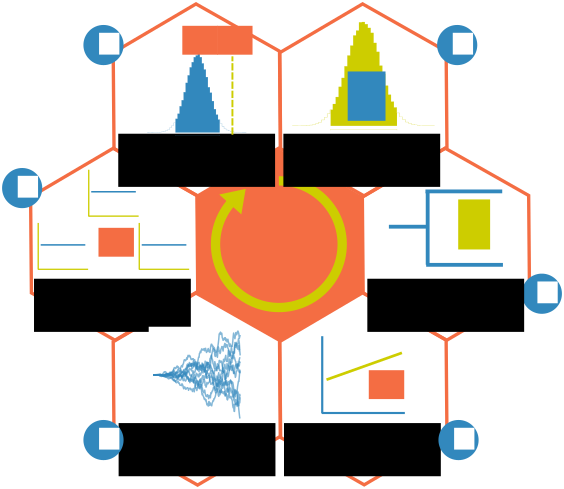
\includegraphics[width=\textwidth]{figs/flow-diagram}
  \caption[Schematic of framework for assessing model adequacy]{Schematic diagram representing our approach for assessing model adequacy. (1) Fit a model of trait evolution to the data; (2) use the estimated model parameters to build a unit tree; (3) compute the contrasts from the data on the unit tree and calculate a set of test statistics $\mathcal{T}_X$; (4) simulate a large number of datasets on the unit tree, using a BM model with $\sigma^2= 1$; (5) calculate the test statistics on the contrasts of each simulated dataset $\mathcal{T}_Y$; and (6) compare the observed and simulated test statistics. If the observed test statistic lies in the tails of the distribution of simulated test statistics the model can be rejected as inadequate. The rotational circle in the center of the diagram indicates that assessing model adequacy is an iterative process. If a model is rejected as inadequate, the next step is to propose a new model and repeat the procedure.}
  \label{fig:flowchart}
\end{figure}

If we have a point estimate of the model parameters, we simulate $Y_1, Y_2, \ldots, Y_m$ on the phylogeny according to $\hat{\theta}$ and $\mathcal{M}$. We then compare a single set of test statistics $\mathcal{T}_X$ calculated from our observed data to the distribution of values for $\mathcal{T}_Y$ computed across all $m$ simulated datasets. In statistical terminology, this procedure is known as parametric bootstrapping. Parametric bootstrapping is likely familiar to phylogenetic biologists in the form of the Goldman-Cox test \citep{Goldman} for assessing the adequacy of sequence evolution models and more recently, the phylogenetic Monte Carlo approach of \citet{Boettiger2012}.

If we have a posterior probability distribution $\Pr(\theta|X, \mathcal{M})$, we can assess model adequacy using posterior predictive simulation \citep{Rubin1984, Gelman1996}. We obtain new datasets by sampling from a second distribution, the posterior predictive distribution
\begin{equation}
\Pr(Y|X,\mathcal{M}) = \int \Pr(Y|\theta, \mathcal{M})\Pr(\theta |X,\mathcal{M})d\theta
\end{equation}
where $\Pr(Y|X,\mathcal{M})$ is the probability of a new dataset $Y$ given $X$ and $\mathcal{M}$, averaged over the posterior distribution of the parameters. (Sampling from $\Pr(Y|X,\mathcal{M})$ is equivalent to simulating datasets using paramaters drawn from the posterior distribution.) Therefore, the datasets $Y_1, Y_2, \ldots, Y_m$ are each generated from different values of $\theta$. Posterior predictive simulation approaches have been previously developed for models in molecular phylogenetics \citep{Bollback2002, Reid2013, Lewis2013, Brown2013}, and recently for PCMs \citep{SlaterPennell}, but have not been widely adopted in either field.

\subsection{Test statistics}
No simulated dataset will ever be exactly the same as our observed dataset. We therefore need to choose informative test statistics in order to evaluate whether the model predicts datasets that are similar to our observed dataset in meaningful ways. As the states at the tips of the phylogeny are not independent--this is why we are using PCMs in the first place!--calculating test statistics on the data directly is not generally informative for models in comparative biology. We account for the non-independence of the observed data by calculating test statistics on the set of contrasts \citep[i.e., ``phylogenetically independent contrasts'';][]{Felsenstein1985} computed at each node. \citep[We refer readers to][for details on how contrasts are calculated.]{Felsenstein1985, Rohlf2001, Blomberg2012} Under Brownian motion (BM) the contrasts will be independent and identically distributed (i.i.d.) according to a normal distribution with mean $0$ and standard deviation $\sigma$ (i.e., contrasts are $\sim \mathcal{N}(0, \sigma)$), where $\sigma^2$ is the BM rate parameter \citep{Felsenstein1985}. This i.i.d. condition allows us to perform standard statistical tests on the contrasts. 

The choice of what test statistics to use for assessing model adequacy is ultimately one of balancing statistical intuition and computational effort. We have chosen the following set of six test statistics to compute on the contrasts because they capture a range of possible model violations and have well-understood statistical properties. All of these essentially evaluate whether the contrasts come from the distribution expected under BM. 

\begin{enumerate}
\item[$M_{\text{SIG}}$] The mean of the squared contrasts. This is equivalent to the REML estimator of the Brownian motion rate parameter $\sigma^2$ \citep{Garland1992, Rohlf2001}. $M_{\text{SIG}}$ is a metric of overall rate. Violations detected by $M_{\text{SIG}}$ indicate whether the overall rate of trait evolution is over- or underestimated.

\item[$C_{\text{VAR}}$] The coefficient of variation (standard deviation/mean) of the absolute value of the contrasts. If $C_{\text{VAR}}$ calculated from the observed contrasts is greater than that calculated from the simulated contrasts, it suggests that we are not properly accounting for rate heterogeneity across the phylogeny. If $C_{\text{VAR}}$ from the observed is smaller, it suggests that contrasts are more even than the model assumes. We use the coefficient of variation rather than the variance because the mean and variance of contrasts can be highly correlated.

\item[$S_{\text{VAR}}$] The slope of a linear model fit to the absolute value of the contrasts against their expected variances \citep[following][]{Garland1992}. Each (standardized) contrast has an expected variance proportional to the sum of the branch lengths connecting the node at which it is computed to its daughter lineages  \citep{Felsenstein1985}. Under a model of BM, we expect no relationship between the contrasts and their variances. We use $S_{\text{VAR}}$ to test if contrasts are larger or smaller than we expect based on their branch lengths. If, for example, more evolution occurred per unit time on short branches than long branches, we would observe a negative slope. If $S_{\text{VAR}}$ calculated from the observed data deviates substantially from the expectations, a likely explanation is branch length error in the phylogenetic tree. 

\item[$S_{\text{ASR}}$] The slope of a linear model fit to the absolute value of the contrasts against the ancestral state inferred at the corresponding node. We estimated the ancestral state using the least-squares method suggested by \citet{Felsenstein1985} for the calculation of contrasts. (We note that this is not technically an ancestral state reconstruction [see Felsenstein, 1985]; it is more properly thought of as a weighted average value for each node.) We used this statistic to evaluate whether there is variation in rates relative to the trait value. For example, do larger organisms evolve proportionally faster than smaller ones?

\item[$S_{\text{HGT}}$] The slope of a linear model fit to the absolute value of the contrasts against node depth \citep[after][]{Purvis1995}. This is used to capture variation relative to time. It is alternatively known as the ``node-height test'' and has been used to detect early bursts of trait evolution during adaptive radiations \citep[see][for uses and modifications of this test]{FreckletonHarvey2006, SlaterPennell}. 

\item[$D_{\text{CDF}}$] The D-statistic obtained from Kolmolgorov-Smirnov test from comparing the distribution of contrasts to that of a normal distribution with mean $0$ and standard deviation equal to the root of the mean of squared contrasts \citep[the expected distribution of the contrasts under BM; see][]{Felsenstein1985, Rohlf2001}. We chose this to capture deviations from normality. For example, if traits evolved via a ``jump-diffusion'' type process \citep{Landis2012}, in which there were occasional bursts of rapid phenotypic evolution \citep{PennellPE}, the tip data would no longer be multivariate normal owing to a few contrasts throughout the tree being much larger than the rest (i.e., the distribution of contrasts would have heavy tails). 

\end{enumerate}

Alternative test statisics are certainly possible. One could, for instance, calculate the median of the squared contrasts, the skew of the distribution of contrasts, etc. If the generating model was known, we could use established procedures for selecting a set of sufficient \citep[or, approximately sufficient;][]{MajoramJoyce} test statistics for that model, as is typically done when computing likelihood ratio tests. However, the aim of our approach is assess the fit of a proposed model without reference to a true model. Our test statistics will detect many types of model misspecification but this does not mean that they will necessarily detect every type of model misspecification. We encourage researchers interested in specific questions to explore alternative test statistics that capture deviations relevant to the problem at hand. 

An additional challenge is determining how to deal with the statistical problems (i.e., inflated Type-1 error rates) that may be introduced when using many test statistics. In our analyses, we chose not to correct our p-values for multiple comparisons (using Bonferroni, false discovery rates, etc.). We did this for a number of reasons. First, our tests are not truly independent and the degree of correlation between test statistics will necessarily depend on the ``true'' model of trait evolution.  Second, as argued by \citet{Gelman2006}, we might be interested in the specific aspects of the data that different from the expectations under the model; rather than focus on whether a model should be accepted or rejected, we ``want to understand the limits of its applicability in realistic replications'' (p. 175). 

\subsection*{Beyond Brownian motion}

All of our test statistics are designed to evaluate the adequacy of a BM model of trait evolution. However, if we propose a different model for the evolution of the trait, such as an Ornstein-Uhlenbeck \citep[OU;][]{Hansen1997} process, then the expected distribution of the contrasts is different. For example, under an OU model, contrasts will not be i.i.d. \citep{Hansen1997}. The expected distribution of contrasts under most models of trait evolution, aside from BM, is not formally characterized and even if it was, this would necessitate a specific set of test statistics for every model proposed.

Our solution to this problem is to create what we term a ``unit tree'', which is a phylogenetic tree transformation that captures the dynamics of trait change under a particular evolutionary model. For a particular evolutionary model $\mathcal{M}$ (with parameter values $\theta$), we define a unit tree as a phylogenetic tree that has the following property: the length of branch $b$, $\nu_b$, is equal to the amount of variance expected to accumulate over $i$ under $\mathcal{M}, \theta$. The variance is standardized, such that the expected distribution of the trait data on the unit tree is equal to that of a Brownian Motion (BM) model with a rate $\sigma^2$ equal to 1.

If the fitted model is adequate, the trait data at the tips of the unit tree will have the same distribution as data generated under a BM process with a rate of 1 and the contrasts will be distributed according to a standard normal distribution (hence the name, unit tree). Creating the unit tree from the estimated model parameters prior to computing the contrasts generalizes the test statistics to most models of quantitative trait evolution \citep[but see][for exceptions]{Landis2012, Landispreprint}. 

We also emphasize that because the contrasts are calculated on the unit tree, the test statistics all must depend on both the data and the model; for this reason, the Bayesian version of our approach produces a distribution of observed test statistics. Once we have created the unit tree from the estimated parameters, new datasets can be simulated under the model simply using a BM process with $\sigma^2 = 1$, which has the added benefit of being computationally efficient.  
The distribution of test statistics calculated on these simulated data sets can then be compared to the test statistics from the observed data. 

\subsection{Details of unit tree construction and the scope of this approach}

Here we formalize our definition of the unit tree and delimit the scope of our approach. Readers can skip this section without missing the main point. A unit tree can be constructed from any evolutionary model where the trait has expected variance-covariance matrix $\mathbf{V}$ that satisfies the (generalized) 3-point condition proposed by \citet{Ho2014} and the data follows a multivariate normal distribution. A matrix $\mathbf{V}$ has a strict 3-point structure if the following condition holds: for any lineages $i,j,k$, the two smallest of $V_{ij}, V_{ik}, V_{jk}$ are equal. Under a simple BM model it is straightforward to show that this condition holds. If $\mathbf{C}$ is the matrix representation of the phylogeny (such that $C_{ij}$ is the shared path length between lineages $i$ and $j$), then by the nature of the tree structure, the 3-point condition will hold for $\mathbf{C}$. Since under BM $\mathbf{V}=\sigma^2\mathbf{C}$, then $\mathbf{V}$ will also be 3-point structured. The same holds true for any evolutionary model that is a branch length transformation of a BM model including the $\lambda, \delta, \kappa$ models \citep{Pagel1997,Pagel1999} and models where rates change through time \citep[the ``Early Burst'' or EB model, also referred to as the Accelerating/Decelerating Change, ACDC, model;][]{Blomberg2003, Harmon2010} or across the tree \citep{Omeara2006, Thomas2006, Eastman2011, Revell2012, motmot}. Standard error can be incorporated into any of these models by simply adding a species-specific scalar to each element of the diagonal. For all of the models where the 3-point condition applies, we can construct a unit tree by setting
\begin{equation}\label{eq:ut}
\nu_{b} = V_{ij} - V_{ik}
\end{equation}
where $V_{ij}$ and $V_{jk}$ are, by the requirements of the 3-point structured condition, equal to one another. Once all branches have been transformed, the contrasts computed on the unit tree will be i.i.d. $\sim \mathcal{N}(0,1)$ under the model in question. 

The OU model of trait evolution also generates 3-point structured matrices when the tree is ultrametric; this is true of both single optimum and multi-optima models \citep{Ho2014}.
However, while the variance structure can easily be transformed to a BM-like tree, the contrasts on this tree will not necessarily be distributed according to a standard normal. For example, while it is often assumed when fitting a single regime OU model that the ancestor is at the optimum trait value \citep[see, for example][]{Harmon2010}, this need not be the case. Furthermore, if there are multiple optima on the phylogeny \citep{Hansen1997, ButlerKing2004, IngramMahler2013, UyedaBayou}, lineages will necessarily be tracking optima that are different from the root state. Therefore, a transformation must also be made to the data in addition to the branch lengths of the phylogeny to produce contrasts that have are i.i.d. according to a standard normal.

To accomplish this, we again turn to the recent work of \citet{Ho2014}. In addition to 3-point structured matrices, Ho and An\'{e} defined a broader condition: a matrix of the form
\[\mathbf{V}=\mathbf{D}_1 \widetilde{\mathbf{V}}\mathbf{D}_2\]
is considered to have a generalized 3-point structure if $\widetilde{\mathbf{V}}$ is 3-point structured and $\mathbf{D}_1$ and $\mathbf{D}_2$ are diagonal matrices. \citet{Ho2014} prove that many phylogenetic models are indeed of this class, including multi-optimum OU models \citep{ButlerKing2004, IngramMahler2013, UyedaBayou}, those with varying rates and models across the tree \citep[e.g.,][]{Beaulieu2012} as well as to OU models fit to non-ultrametric trees. For any model that satisfies the generalized 3-point condition and where the data is assumed to come from a multivariate normal distribution, there exists some transformation to the tree (appling Equation \ref{eq:ut} to $\widetilde{\mathbf{V}}$) and data (using $\mathbf{D}_1$ and $\mathbf{D}_2$) that will produce a unit tree with standard normal contrasts. We note that \citet{Slater2014} recently pointed out that for OU models fit to non-ultrametric trees, there is no valid transformation that can make $\mathbf{V}$ BM-like. While this is indeed correct, it is however, possible to get a BM-like tree by adding a species-specific scalar to the data matrix \citep{Ho2014}. Therefore, once the proper tree and data transformations have been made, all the test statistics described above can apply.

The above also applies to phylogenetic regression models \citep{Grafen1989, Lynch1991, MartinsHansen1997} of the form
\[Y = \beta_0 + \beta_1 X + \epsilon.\]
In these models, the error variance is structured by phylogeny assuming some model of trait evolution such that $\epsilon \sim \mathcal{N}(\mathbf{0}, \mathbf{V})$. In these regression models $\mathbf{V}$ represents the variance-covariance matrix of the residuals rather than the traits \citep{Rohlf2001}. Therefore if $\mathbf{V}$ is either 3-point or generalized 3-point structured, the tree (and possibly data) can be transformed such that the contrasts on the residuals will be i.i.d. standard normal. This fact allows researchers to use our approach to assess the adequacy of a trait model for understanding correlations between traits. We note however that as $\mathbf{V}$ only affects the error structure for these models, alternative approaches \citep[see for example][ch. 6]{Gelmanbook} will be required to assess the adequacy of the mean structure $Y = \beta_0 + \beta_1X$ of the model.

\subsection{Simulations}

As a verification of our method, we conducted a brief simulation study. We focused here on assessing Type-1 error rates. As above, we emphasize that these are not necessarily the most important quantities when thinking about model adequacy, but they do provide a useful metric for demonstrating that our code is functioning correctly. The philosophy behind approaches such as ours is that the ``true'' model is outside of the candidate set. We want to ask whether a given model can adequately describe the variaton in the data. If it does, we can consider it statistically adequate even if it is not the true model or even the best model in our set (see Discussion for comments on the relationship between model adequacy and model selection). Furthermore, while it is certainly interesting to examine what types of deviations in model space produce what types of deviations in the various test statistics, the number of possible simulation conditions is infinitely broad.

We simulated data under BM, single-optimum OU, and EB (the same models we used in the analysis; see below). For each set of simulating conditions, we simulated trees of 50, 100, and 200 taxa under a pure-birth process, then rescaled the tree to be unit height. For BM, we set $\sigma^2=1$. For OU, we used $\sigma^2=1$ but varied the ``selection'' parameter $\alpha$ ($\alpha=\lbrace 1,2,4 \rbrace$). For EB, we again set $\sigma^2$ to be 1 and varied $a$, the exponential rate of decline \citep[see][for details]{Harmon2010, SlaterPennell}, was set to be $a=\lbrace \log(0.01), \log(0.02), \log(0.04) \rbrace$. For each parameter combination, we ran 500 simulations under two sets of conditions: (1) assuming no measurement error; and (2) assuming known error rates of 5\% of the expected variance in trait values across the phylogeny. We then fit the corresponding model using maximum likelihood and evaluated the Type-1 error under each set of conditions. All simulations were conducted using \textsc{diversitree} \citep{FitzJohn2012}.


\section{The adequacy of models for the evolution of plant functional traits}

\subsection{Data}
%% Number of Angiosperms in big tree: 30535
We used a phylogeny of Angiosperms, containing 30,535 species, from a recent study by \citet{Zanne2013}.  We conducted all analyses on the MLE of the phylogeny (available on DRYAD, doi:10.5061/dryad.63q27/3). We used existing large datasets on three functionally important plant traits: specific leaf area (SLA, defined as fresh area/dry mass), seed mass, and leaf nitrogen content (\% mass). Seed mass is a crucial part of species' life-history strategy \citep{Leishman2000, Westoby2002} and SLA and leaf nitrogen content are important and widely measured components of species' carbon capture strategies \citep{Wright2004}. Understanding the macroevolutionary patterns of these three traits can provide key insights into the evolutionary processes that have shaped much of plant diversity \citep{ksi}. The SLA and leaf nitrogen data comes from \citet{Wright2004} with additional SLA data from the LEDA project \citep{Kleyer2008}. Seed mass data comes the Kew database \citep{Kew2008}. We used an approximate grepping approach to find and correct spelling mistakes and synonymy tools from \citet{ThePlantList} to match the trait databases to the Zanne et al. phylogeny. 
%% Full data stats
%% SLA
%% in dataset: 3293
%% matched to tree: 2200
%% Seed mass
%% in dataset: 22817
%% matched to tree: 11107
%% Leaf N
%% in dataset: 1574
%% matched to tree: 936
The full data set includes 3293 species for SLA, of which 2200 match species in the \citet{Zanne2013} tree. For seed mass, the dataset included 22,817 species with 11,107 matched the phylogeny. For leaf nitrogen content, we have data for 1574 species with 936 included in the tree. 
%
See \texttt{https://github/richfitz/modeladequacy} for specific locations and scripts to access and process the original data. 

We log-transformed all data prior to analysis. We did this for biological reasons rather than to conform the data to the assumptions of the model \citep{Houle2011}. It is more meaningful to model trait evolution as a multiplicative process rather than an arithmetic one. An increase of two grams is much more significant for the seed of an orchid than the seed of a palm tree. However, we should recognize that both of these rationales are essentially statements about model adequacy and thus the validity of the log transformation can be quantitatively assessed. We ran our analysis on both the raw and log transformed data.

Because the vast majority of the species are only represented by a single
record, it was not possible to use a species-specific estimate of
trait standard error (SE) to account for either measurement error or
intraspecific variation.  As an alternative, we estimated a single SE for each trait
by calculating the mean
standard deviation for all species for which we had multiple
measurements. The assumption of a constant SE across all species is
unlikely to be correct, but even an
inaccurate estimate of error is better than assuming none at all
\citep{Hansen2012SysBio}. 

\subsection{Analysis}

We first matched our trait data to the whole phylogeny and then extracted subclades from this dataset in a three ways: (1) by family; (2) by order; and (3) by cutting the tree at 50 My intervals and extracting the most inclusive clades (named or unnamed) for which the most recent common ancestor of a group was younger than the time-slice. 
%% Crown age of angiosperms: 243.2697 my
(The crown age of Angiosperms is estimated to be $\sim$243 my in the MLE tree and the tree was cut at 50, 100, 150, and 200my.) We kept only subclades for which there was at least 20 species present in both the phylogeny and trait data so that we had a reasonable ability to estimate parameters and distinguish between models \citep{Boettiger2012, SlaterPennell}. 
%% Number of clades per trait
%% SLA: 72
%% Seed mass: 226
%% leaf n: 39
For SLA, this left us with 72 clades, seed mass, 226 clades, and leaf nitrogen content, 39 clades (337 in total). We note that these datasets are not independent as many of the same taxa were included in family, order and multiple time-slice subtrees. 

Following \citet{Harmon2010}, we considered three simple models of trait evolution: (1) BM, which can be associated with genetic drift \citep{Lande1976, Felsenstein1988, LynchHill1986, Lynch1990, HansenMartins1996}, randomly-varying selection \citep{Felsenstein1973}, or the summation of many independent processes over macroevolutionary time \citep{HansenMartins1996, Uyeda2011, PennellPE}; (2) single optimum OU, which is often assumed to represent stabilizing selection \citep[following][]{Lande1976}, though we think a more meaningful interpretation is that it represents an ``adaptive zone'' \citep{Hansen2012book, PennellHarmon}; and (3) EB, which was developed as a phenomenological representation of a niche-filling process during an adaptive radiation \citep{Blomberg2003, Harmon2010}. We fit each of these models to all 337 subclades in our dataset. We then used the approach we developed to assess the adequacy of each fitted model. 

All of the analyses conducted in this paper were conducted using both likelihood and Bayesian inference. We did so to demonstrate the scope of our approach and because both ML and Bayesian inference are commonly used in comparative biology. We emphasize that our approach is not tied to any single statistical paradigm.

For the likelihood analyses, we fit the three models (BM, OU, and EB) using ML with the \textsc{diversitree} package \citep{FitzJohn2012}. We calculated the AIC score for each model. We then constructed a unit tree for each subtree, trait and model combination using the maximum likelihood estimates of the parameters. We calculated the six test statistics described above ($M_{\text{SIG}}$, $C_{\text{VAR}}$, $S_{\text{VAR}}$, $S_{\text{ASR}}$, $S_{\text{HGT}}$, $D_{\text{CDF}}$) on the contrasts of the data. We simulated 1000 datasets on each unit tree using a BM model with $\sigma^2=1$ and calculated the test statistics on the contrasts of each simulated data set. 

For the Bayesian analysis, we fit the same models as above using a MCMC approach, sampling parameter values using slice sampling \citep{Nealslice}, as implemented in  \textsc{diversitree} \citep{FitzJohn2012}. For the BM model we set a broad uniform prior on $\sigma^2 \sim \mathcal{U}[0, 2]$, the upper bound being substantially larger than the ML estimate of $\sigma^2$ for any clade. For the OU model, we used the same prior for $\sigma^2$ and drew $\alpha$ values, the strength of attraction to the optimum, from a Lognormal$(\mu=\log(0.5),\sigma= \log(1.5))$ distribution. A complication involved in fitting OU models is deciding what assumptions to make about the state at the root $z_0$. Here, we follow other authors \citep{ButlerKing2004,Harmon2010} and assume that $z_0$ is at the optimum. For the EB model, we again used the same prior for $\sigma^2$ and a uniform prior on $a$, the exponential rate of decrease in $\sigma^2$, such that $a \sim \mathcal{U}[-1, 0]$ \citep[the minimum value is much more negative than we would typically expect;][]{SlaterPennell}.

Again, for each model/trait/subtree combination, we ran a Markov chain for 10,000 generations. Preliminary investigations demonstrated that this was more than sufficient to obtain convergence and proper mixing for these simple models. After removing a burn-in of 1000 generations, we calculated the Deviance Information Criterion \citep[DIC, a Bayesian analog of AIC;][]{dic} for each model. We drew 1000 samples from the joint posterior distribution. For each of the sampled parameter sets, we used the parameter values to construct a unit tree and calculated our six test statistics on the contrasts. We then simulated a dataset on the same unit tree and calculated the test statistics on the contrasts of the simulated data. 

In the likelihood analyses, for each dataset, we had one set $\mathcal{T}_X$ of observed test statistics and a 1000 sets $\mathcal{T}_{Y,1}, \mathcal{T}_{Y,2}, \ldots, \mathcal{T}_{Y,1000}$ of test statistics calculated on data simulated on the same unit tree. In the Bayesian version, we had 1000 sets of observed test statistics $\mathcal{T}_{X,1}, \mathcal{T}_{X,2}, \ldots, \mathcal{T}_{X,1000}$ using a different unit tree for each set and 1000 sets of simulated test statistics $\mathcal{T}_{Y,1}, \mathcal{T}_{Y,2}, \ldots, \mathcal{T}_{Y,1000}$, each $\mathcal{T}_{Y,i}$ corresponding to the unit tree used to compute $\mathcal{T}_{X,i}$.
 
For both types of analyses, we report two-tailed $p$-values (i.e., the probability that the observed that a simulated test statistic was more extreme than the observed). As a multivariate measure of model adequacy, we calculated the Mahalanobis distance, a scale-invariant metric, between the observed test statistics and the mean of our simulated test statistics, taking into account the covariance structure between the simulated test statistics. We took the log of the \text{KS} D-statistic, $D_{\text{CDF}}$, as the Mahanalobis measure assumes data is multivariate normal and the D-statistic is bounded between 0 and 1. For the Bayesian analyses, we report the mean of the distribution of Mahalanobis distances. All analyses were conducted in R v3.0.2. Scripts to fully reproduce all analyses are available at \texttt{https://github.com/richfitz/modeladequacy}.
  
\subsection{A case study: seed mass evolution in the Meliaceae and Fagaceae }
As an illustration of our approach, we present a case study examining seed mass evolution in two tree families, the Meliaceae, the ``mahogany family'', and Fagaceae, which contains oaks, chestnuts and beech trees. The trait data and phylogeny for both groups are subsets of the larger dataset used in the analysis. Superficially, these datasets are quite similar. Both are of similar size (Meliaceae: 44 species in the dataset, 550 in the clade; Fagaceae: 70 species in the dataset and 600 in the clade), age (crown age of Meliaceae: $\sim$53my; Fagaceae: $\sim$40my) and are ecologically comparable in terms of dispersal strategy and climatic niche. 

As described above, we fit three simple models of trait evolution (BM, OU, EB) to both datasets using ML and computed AIC weights \citep[AIC$_w$;][]{Akaike1974, aicweight} for the three models. For both datasets, an OU model was overwhelmingly supported (AIC$_w$ $>0.97$ for both groups). Therefore, looking only at relative model support, we might conclude that similar evolutionary processes are important in these two clades of trees.

% RGF: Belongs in the results?
%% Meliaceae seedmass p-values (OU)
%%    m.sig     c.var     s.var     s.anc     s.hgt     d.cdf 
%% 0.9210789 0.6053946 0.979021 0.4815185 0.1698302 0.6573427 
%%
%% Fagaceae seedmass p-values (OU)
%%    m.sig     v.pic     s.var     s.asr       s.hgt     d.cdf 
%% 0.2977023 0.8371628 0.000000 0.07392607 0.01398601 0.5514486
Examining model adequacy provides a different perspective. We took the MLE of the parameters from the OU models for each dataset and constructed a unit tree based on those parameters. We calculated our six test statistics on the contrasts of the data, then simulated 1000 datasets on the unit tree and calculated the test statistics on the contrasts of each simulated dataset (figure \ref{fig:two-clades}). 

\begin{figure}[p]
  \centering
  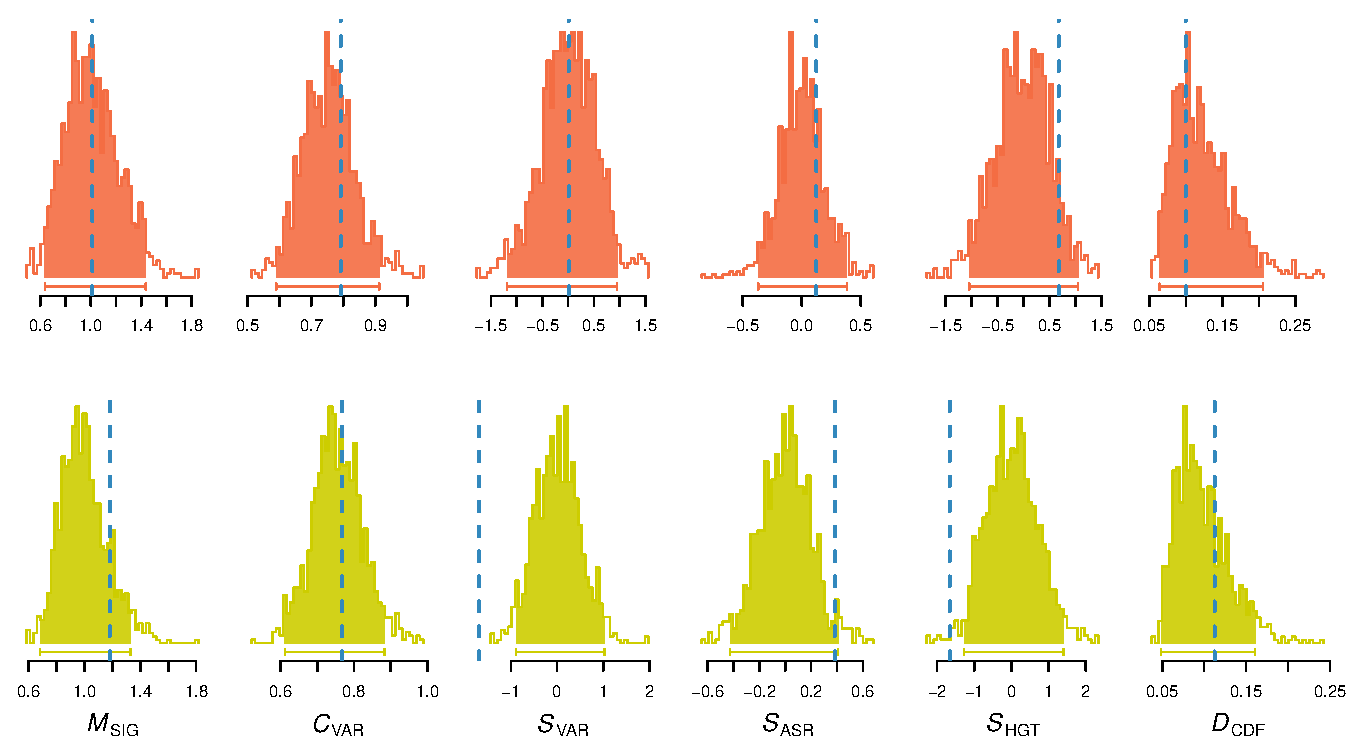
\includegraphics[width=\textwidth]{figs/two-clades}
  \caption[Seed mass evolution in Meliaceae and Fagaceae]{Illustration of our approach to model adequacy. We fit three models (BM, OU, and EB) to seed mass data from two different tree families, the Meliaceae (top panel, red) and the Fagaceae (bottom panel, yellow). In both cases, an OU model (analyzed here) was strongly supported when fit with ML. The plotted distributions are the test statistics ($M_{\text{SIG}}, C_{\text{VAR}}, S_{\text{VAR}}, S_{\text{ASR}}, S_{\text{HGT}}, D_{\text{CDF}}$) calculated from the contrasts of the simulated data; the bars underneath the plots represent 95\% of the density. The dashed vertical lines are the values of the test statistics calculated on the contrasts of the observed data. Using our test statistics, an OU model appears to be an adequate model for the evolution of seed mass in the Meliaceae; for all of the test statistics, the observed test statistic lies in the middle of the distribution of simulated test statistics. For the Fagaceae, the slopes of the contrasts against their expected variances $S_{\text{VAR}}$ and node height $S_{\text{HGT}}$ are much lower than the expectations under the model.}
  \label{fig:two-clades}
\end{figure}

For seed mass evolution in Meliaceae, the OU model was an adequate model; all six observed test statistics were in the middle of the distribution of simulated test statistics ($M_{\text{SIG}}: p=0.921$, $C_{\text{VAR}}: p=0.605$, $S_{\text{VAR}}: p=0.979$, $S_{\text{ASR}}:p=0.485$, $S_{\text{HGT}}: p=0.170$, $D_{\text{CDF}}: p=0.657$). In contrast, for Fagaceae we found that the test statistics calculated with an OU model lay outside the expected values for $S_{\text{VAR}}$ ($p \approx 0$) and $S_{\text{HGT}}$ ($p = 0.014$) suggesting that the process of evolution that gave rise to this data was more complex that that captured by a simple OU process. Specifically, we would infer that rates of evolution depend on the length of the branches ($S_{\text{VAR}}$), which may indicate phylogenetic error, and that the model is failing to fully capture variation through time ($S_{\text{HGT}}$. The rest of the observed test statistics did not differ significantly from the simulated test statistics ($M_{\text{SIG}}: p=0.298$, $C_{\text{VAR}}:p=0.837$, $S_{\text{ASR}}:p=0.074$, $D_{\text{CDF}}: p=0.551$). This example illustrates the distinction between the conventional approach to model selection in PCMs and model adequacy. Selecting amongst a limited pool of models does not give a complete picture of the amount of variation that a chosen model is actually capturing.


\section{Results}

\subsection{Simulations}

In our simulations, we found that when we assessed the adequacy of the generating model, all of the test statistics showed Type-1 errors that were consistently around or less than 0.05. This was true across models, parameters, tree sizes and did not depend on whether we included a known SE or not (figures \ref{fig:bm-sim}, \ref{fig:ou-sim}, and \ref{fig:eb-sim}). These results demonstrate that our unit tree construction is working properly; if the MLE is equal to the generating value, then the constrasts will be i.i.d. $\mathcal{N}(0,1)$ and standard normal statistical properties will apply. Some of the test statistics are very conservative (have very low Type-1 error rates) under some models. We are not aware of any general statistical theory that will allow us to predict the conditions under which a test statistic will have low power to detect deviations from the expected distributions. However, there is an intiutive explanation for this pattern. Consider for example, our test statistic $M_{\text{SIG}}$. As mentioned above, this is equivalent to the REML estimate of $\sigma^2$. When we fit BM (or, a more general model, of which BM is a special case), and then rescale the tree with $\hat{\sigma^2}$, the observed contrasts on the unit tree will effectively be minimized with respect to this quantity and all of the contrasts on the simulated dataset will tend to be larger than our observed contrasts. So if the quantity captured by the test statistic is tightly correlated with one of the parameters being optimized in the model, this test statistic will tend to have low power to detect deviations from this model.

\begin{figure}[p]
  \centering
  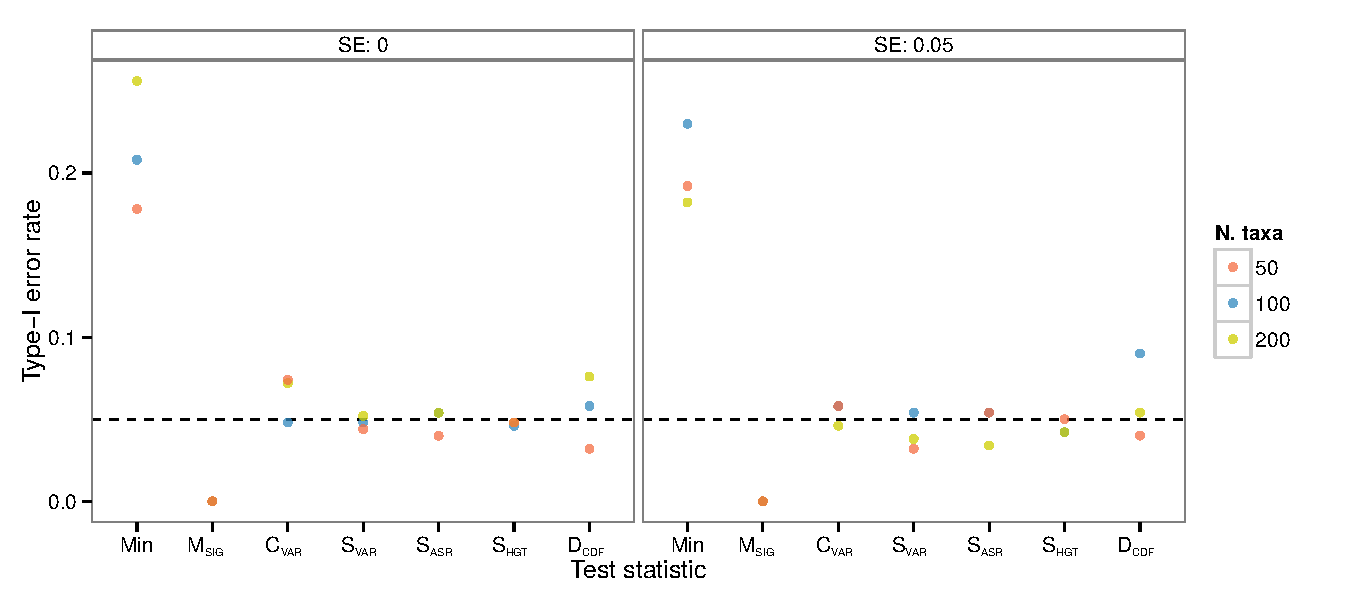
\includegraphics[width=\textwidth]{figs/bm-sim-res}
  \caption[Type-1 error rates for data simulated under Brownian motion]{Type-1 error rates for data simulated under a Brownian motion (BM) model. We simulated 500 datasets under for 3 different tree sizes ($N=\lbrace 50, 100, 200 \rbrace $, represented by the different colors) and two known values of standard error ($0$ and $0.05$, left and right panel, respectively). The Type--1 error rates for each test statistic are consistently around or lower than $0.05$ threshold. However, the frequency at which \emph{at least one} of the test statistics deviated significantly from the expectations (the variable ``min'' on the left side of each plot) was substantially greater, rising to above $0.2\%$ in some cases. See text for why we decided against correcting for the effect of multiple comparisons in the analysis.}
  \label{fig:bm-sim}
\end{figure}

\begin{figure}[p]
  \centering
  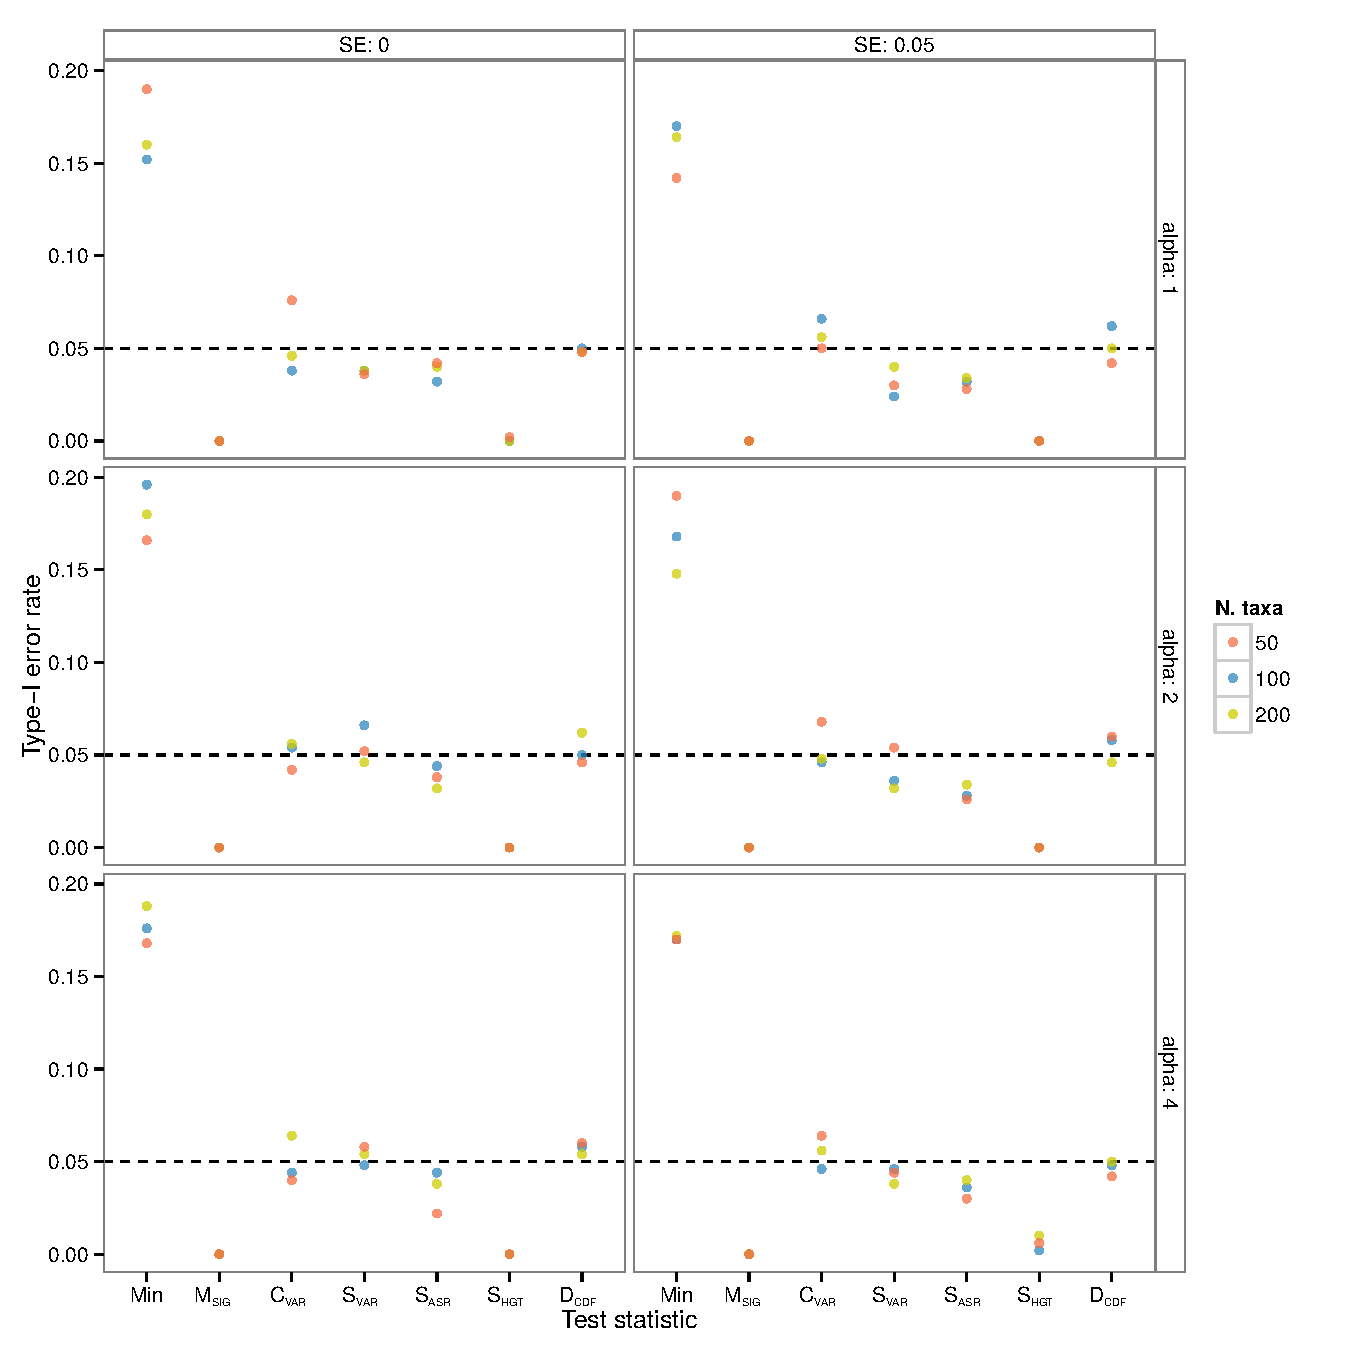
\includegraphics[width=\textwidth]{figs/ou-sim-res}
  \caption[Type-1 error rates for data simulated under Ornstein-Uhlenbeck]{Type-1 error rates for data simulated under an Ornstein-Uhlenbeck (OU) model. We simulated 500 datasets under for 3 different tree sizes ($N=\lbrace 50, 100, 200 \rbrace$, represented by the different colors) and two known values of standard error ($0$ and $0.05$, left and right panel, respectively). We also simulated under three values for the $\alpha$ parameter ($\alpha=\lbrace 1,2,4 \rbrace$, top, middle and bottom panel), representing phylogenetic half-lives of $69\%$, $35\%$, $17\%$ of total tree depth, respectively.  The Type--1 error rates for each test statistic are consistently around or lower than $0.05$ threshold. However, the frequency at which \emph{at least one} of the test statistics deviated significantly from the expectations (the variable ``min'' on the left side of each plot) was substantially greater, approaching $0.2\%$ in some cases. See text for why we decided against correcting for the effect of multiple comparisons in the analysis.}
  \label{fig:ou-sim}
\end{figure}

\begin{figure}[p]
  \centering
  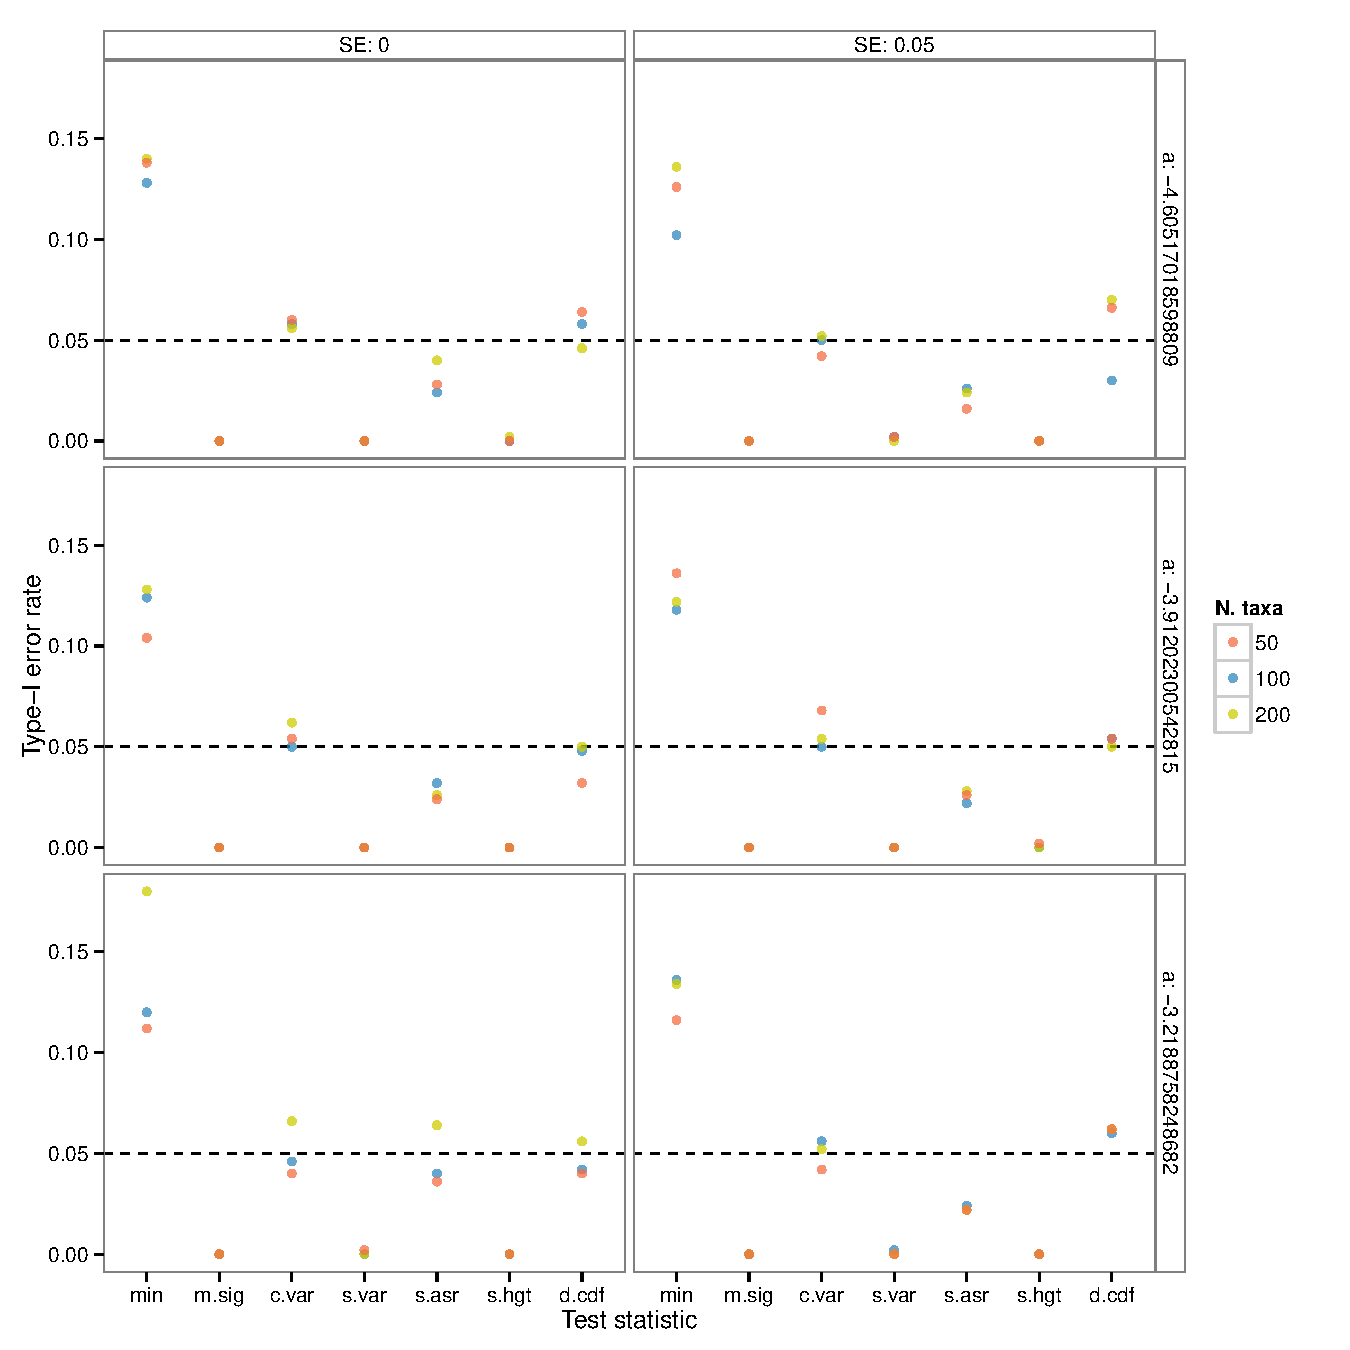
\includegraphics[width=\textwidth]{figs/eb-sim-res}
  \caption[Type-1 error rates for data simulated under Early Burst]{Type-1 error rates for data simulated under an Ornstein--Uhlenbeck (OU) model. We simulated 500 datasets under for 3 different tree sizes ($N=\lbrace 50, 100, 200 \rbrace$, represented by the different colors) and two known values of standard error ($0$ and $0.05$, left and right panel, respectively). We also simulated under three values for the exponential rate of slowdown, $a$ ($a=\lbrace \log(0.01),\log(0.02),\log(0.04) \rbrace$, top, middle and bottom panel), which translate to the rate of trait evolution halfing every $0.15$, $0.17$, and $0.21$ time units, respectively (note that the tree was scaled so the total depth was equal to unity).  The Type--1 error rates for each test statistic are consistently around or lower than $0.05$ threshold. However, the frequency at which \emph{at least one} of the test statistics deviated significantly from the expectations (the variable ``min'' on the left side of each plot) was substantially greater, approaching $0.15\%$ in some cases. See text for why we decided against correcting for the effect of multiple comparisons in the analysis.}
  \label{fig:eb-sim}
\end{figure}

We also found that by using multiple test statistics and reporting a Type-1 error if \emph{any} of the test statistics deviated significantly from expectations, the error rate increased substantially (up to around 20\% under some conditions). However, as we discuss above, we do not think that this is necessarily a defect of the analysis and are not overly concerned with this error rate. Looking at what test statistics were violated and how they were violated is much more meaningful than simply rejecting or accepting a model based on the overall $p$-value. Furthermore, the degree to which the Type-1 error rate will rise with multiple comparisons will be a complex function of the generating model and the size of the dataset and there is no suitable general correction that we know of.

\subsection{Models for the evolution of Angiosperm functional traits}

\subsubsection{Maximum likelihood}

Across the 337 subclades, we found widespread support for OU
%% n. clades OU best supported model: 235
models. For 236 of clades, OU had the highest AIC$_w$.
%% n. clades OU supported with 100% aicw: 27
%% n. clades OU supported with >75% aicw: 189
OU had $\sim$100\% of the AIC$_w$ in 27 clades and $>$75\% of the weight in 189 clades (figure \ref{fig:aic-support}). Consistent with \citet{Harmon2010} we found very little support for EB models (only 6 clades supported EB with $>$75\% AIC$_w$), suggesting that ``early bursts'' of trait evolution are indeed be rare in comparative data \citep[but see][]{SlaterPennell}. Larger clades commonly had
%% n. clades with more than 100 taxa: 101
%% of these, how many had a single model with >90% support: 44
very high support for a single model (of the 101 clades consisting of more than 100 taxa, 44 had $>$90\% of the AIC weight on a single model),
%% of these 58, how many were OU: 42
and that was overwhelmingly likely to be an OU model (42/44 clades).

\begin{figure}[p]
  \centering
  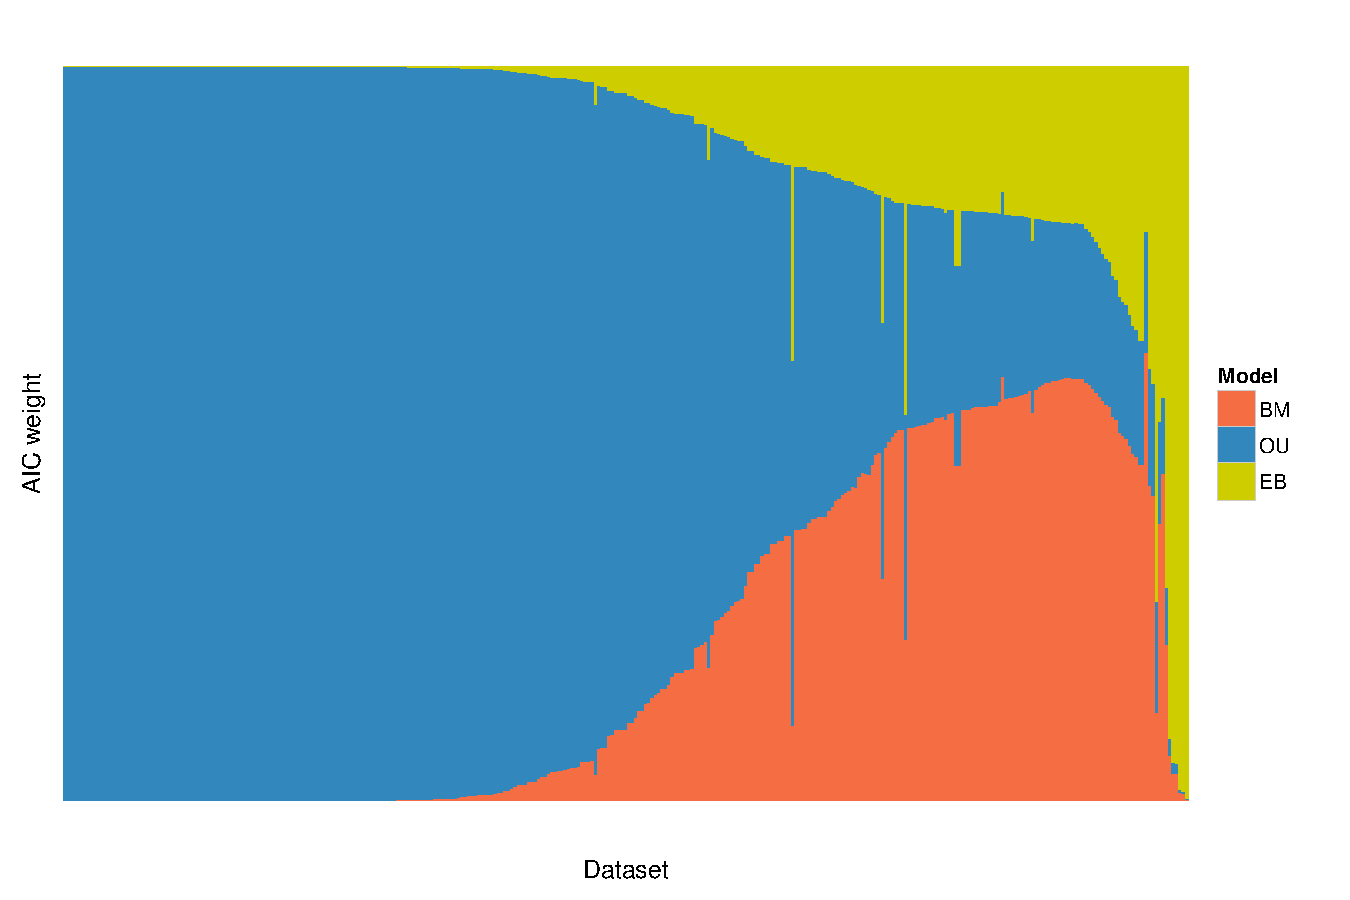
\includegraphics[width=\textwidth]{figs/aic-support}
  \caption[Relative support for models across Angiosperm datasets (ML)]{The relative support, as measured by AIC weight, for the three models used in our study (BM, OU, and EB) across all 337 datasets. An OU model is highly supported for a majority of the datasets.}
  \label{fig:aic-support}
\end{figure}
 

We limit our analyses of model adequacy to only the most highly supported model in the candidate set, as supported by AIC. We did this to present a best-case scenario; if a model had very little relative support, it would be unremarkable if it also had poor adequacy \citep[but see][]{Ripplinger2010}. Even considering only the best of the set, in general, the datasets often deviated from the expectations of the model in at least some ways (figure \ref{fig:pvalues}). 
%% SLA data for 72 clades
%% rejected by at least one ss: 32
%% rejected by at least two ss: 22
%% rejected by at least three ss: 15
Of the 72 comparative datasets of SLA, we detected deviations from the expectations in 32 datasets (using a cut-off of $p= 0.05$), 33 by at least two, and 17 by three or more. 
%% Seed mass data for 226 clades
%% rejected by at least one ss: 153
%% rejected by at least two ss: 95
%% rejected by at least three ss: 65
Results were similar in the seed mass data (of the 226 seed mass datasets, we detected deviations in 153 datasets with at least one test statistic, 128 by at least two and 74 by three or more) and leaf nitrogen content 
%% Leaf nitrogen data for 39 clades
%% rejected by at least one ss: 19
%% rejected by at least two ss: 12
%% rejected by at least three ss: 8
(of the 39 datasets, we detected deviations in 19 by at least one, 24 by at least two, and 11 by three or more test statistic). 
%% statistics which were most often violated
%% rejected by m.sig: 39
%% rejected by c.var: 163
%% rejected by s.var: 118
%% rejected by s.asr: 84
%% rejected by s.hgt: 54
%% rejected by d.ks: 67

\begin{figure}[p]
  \centering
  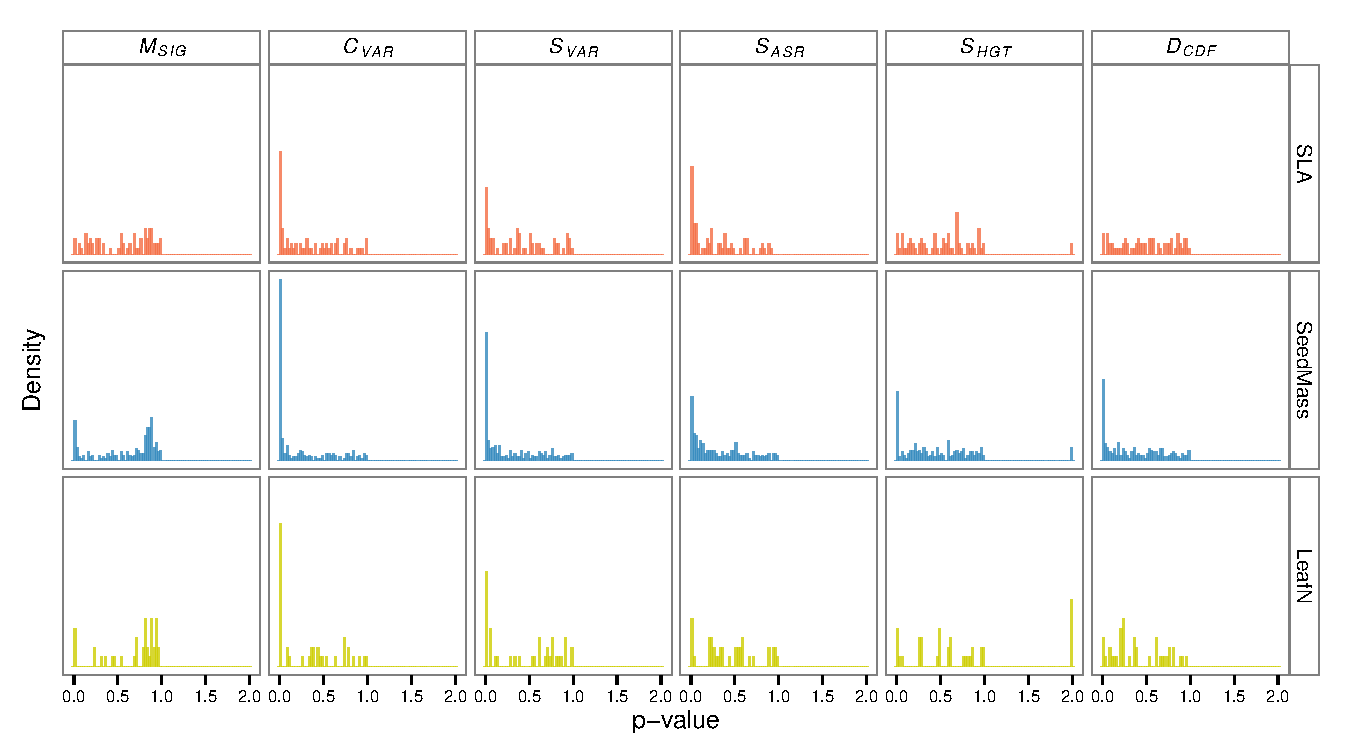
\includegraphics[width=\textwidth]{figs/pval-hist-ml}
  \caption[Distribution of $p$-values for test statistics (ML)]{The distribution of $p$--values for our six test statistics over all 337 datasets in our study after fitting the models using ML. The $p$--values are from applying our model adequacy approach to the best supported of the three models (as evaluated with AIC). Many of the datasets deviate from the expectations under the best model along a variety of axes of variation. Deviations are particularly common for the coefficient of variation $C_{\text{VAR}}$ and the slope of the contrasts against their expected variances $S_{\text{VAR}}$.}
  \label{fig:pvalues}
\end{figure}

Some test statistics were much more likely to detect model violations than others. In 163 cases $C_{\text{VAR}}$ revealed the data deviated significantly from the expections of the best model. In 118 cases, $S_{\text{VAR}}$ did. The rate of deviation was much somewhat lower for the other test statistics ($M_{\text{SIG}}$: 39, $S_{\text{ASR}}$: 84, $S_{\text{HGT}}$: 54, $D_{\text{CDF}}$: 67).

%% The number of datasets which were adequately modeled: 133
Across all 337 datasets, 133 are adequately modeled by either BM, OU or EB. As stated above, the numbers of models that showed deviations with at least one test statistic may be somewhat overinflated. However, the proportion of clades in which p-values were less than 0.05 is much, much greater than the error rates we found in our simulations. And the proportions for each individual test statistic is much higher than would be expected by chance. 

As the subclades are not independent (overlapping sets of taxa are present in family, order and time-slice phylogenies), conventional statistics, such as linear regression, are not straightforward to apply across datasets. Nonetheless, the trend is clear: the larger the phylogeny, the more likely OU is to be highly supported and the more likely the model is to be inadequate. There is a strong relationship between the size of a subclade and the overall distance between observed and simulated test statistics, as measured by the Mahanalobis distance (figure \ref{fig:size-adequacy}). This is not simply an artifact of conducting the analyses using a larger number of contrasts for the test statistics-if the model was adequate at all scales, there would be no relationship between the Mahalanobis distance and the size of the phylogeny. Because larger clades also tended to support a single model, the datasets for which the best model had a very poor absolute fit also had the most substantial difference between the relative fits of the three models (figure \ref{fig:supp-ad-aic}). There was a much weaker relationship between clade age and model adequacy (figure \ref{fig:supp-age-ml}).

\begin{figure}[p]
  \centering
  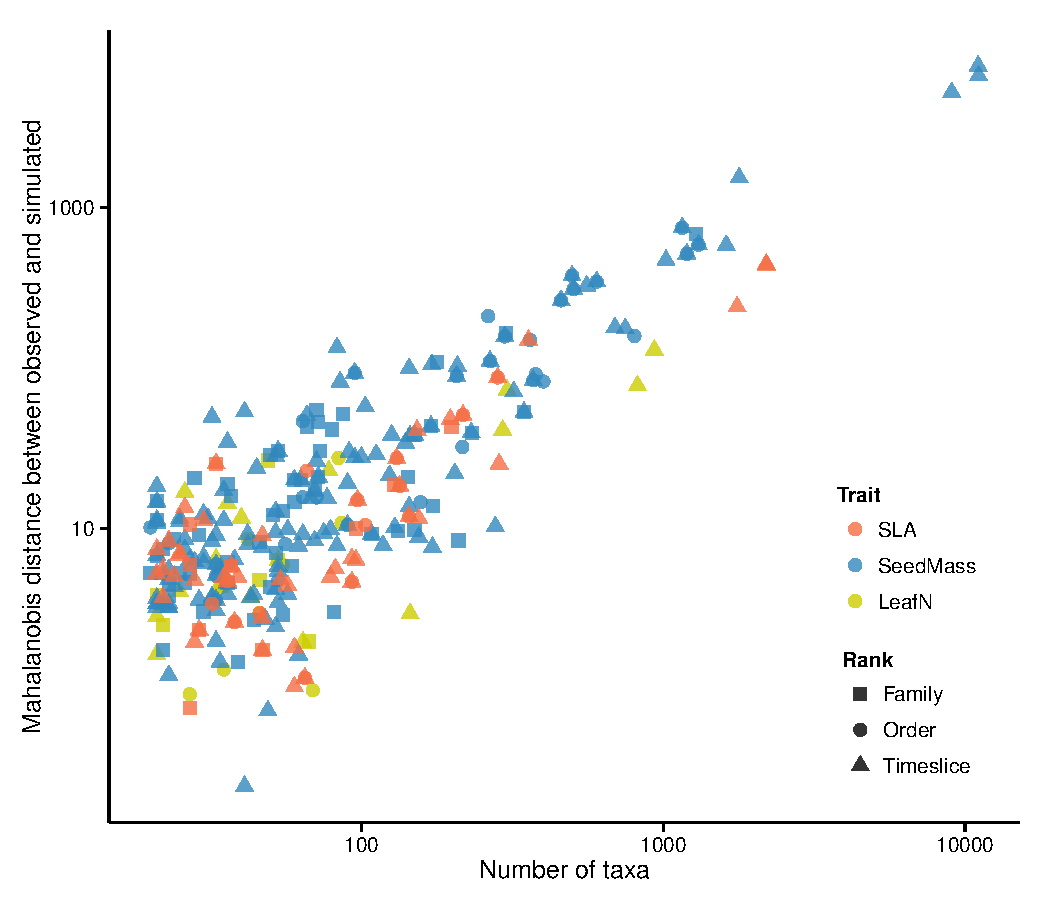
\includegraphics[width=\textwidth]{figs/ad-size-ml}
  \caption[Model adequacy versus clade size (ML)]{The relationship between clade size and a multivariate measure of model adequacy. The Mahalanobis distance is a scale--invariant metric that measures the distance between the observed and simulated test statistics, taking into account the covariance between test statistics. The greater the Mahalanobis distance, the worse the model captures variation in the data. Considering only the best supported model for each clade (as chosen by AIC), there is a striking relationship between the two --- the larger the dataset, the worse the models performed (note the logarithmic scale). If the models were equally likely to be adequate at all scales, we would expect no relationship.}
  \label{fig:size-adequacy}
\end{figure}


\begin{figure}[p]
  \centering
  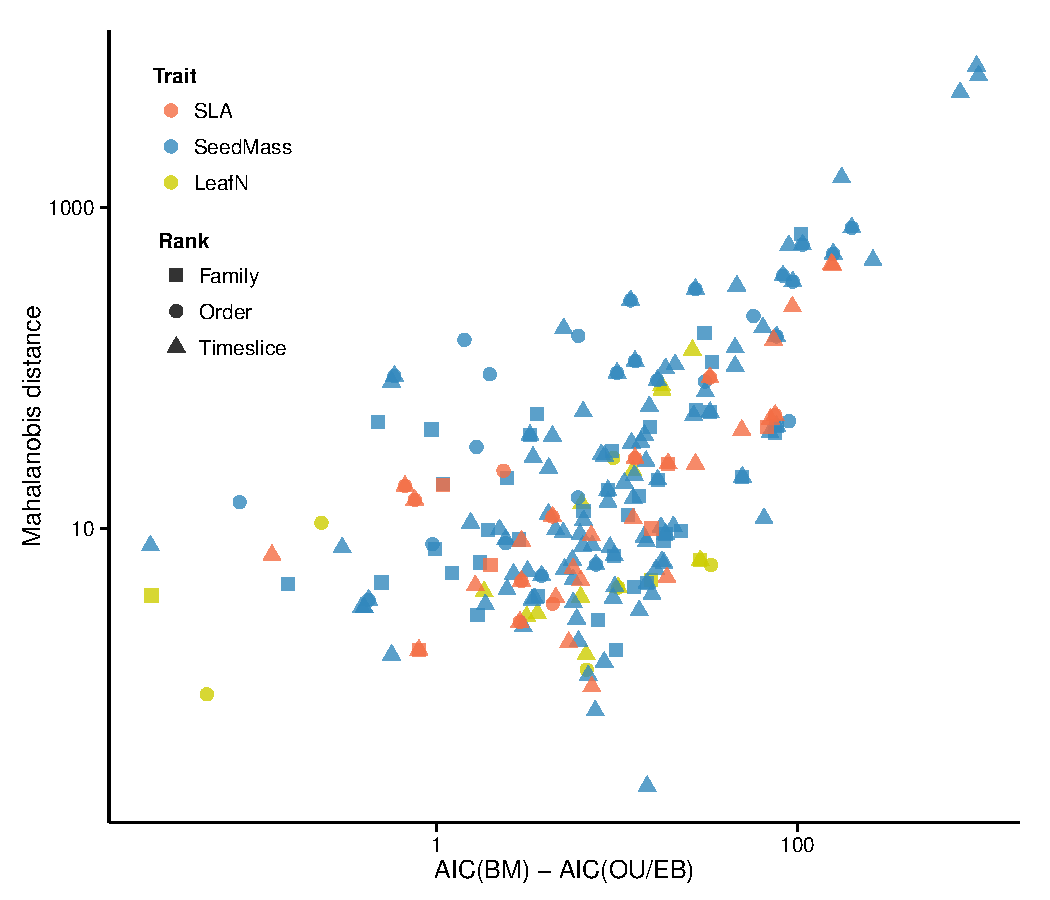
\includegraphics[width=\textwidth]{figs/ad-aic}
  \caption[Model adequacy versus model support (ML)]{The relationship between relative and absolute fit. For every clade for which a more complex model (OU, EB) was favored over BM using AIC, the Mahalanobis distance between the observed test and simulated test statistics is plotted against the improvement in AIC for the more complex model compared to BM. (Note that as all AIC values were negative, larger differences mean greater relative support). The greater the relative fit of a more complex model, the more likely the model was to be inadequate. This result in primarily driven by clade size but serves to emphasize the distinction between relative and absolute fit.}
  \label{fig:supp-ad-aic}
\end{figure} 

\begin{figure}[p]
  \centering
  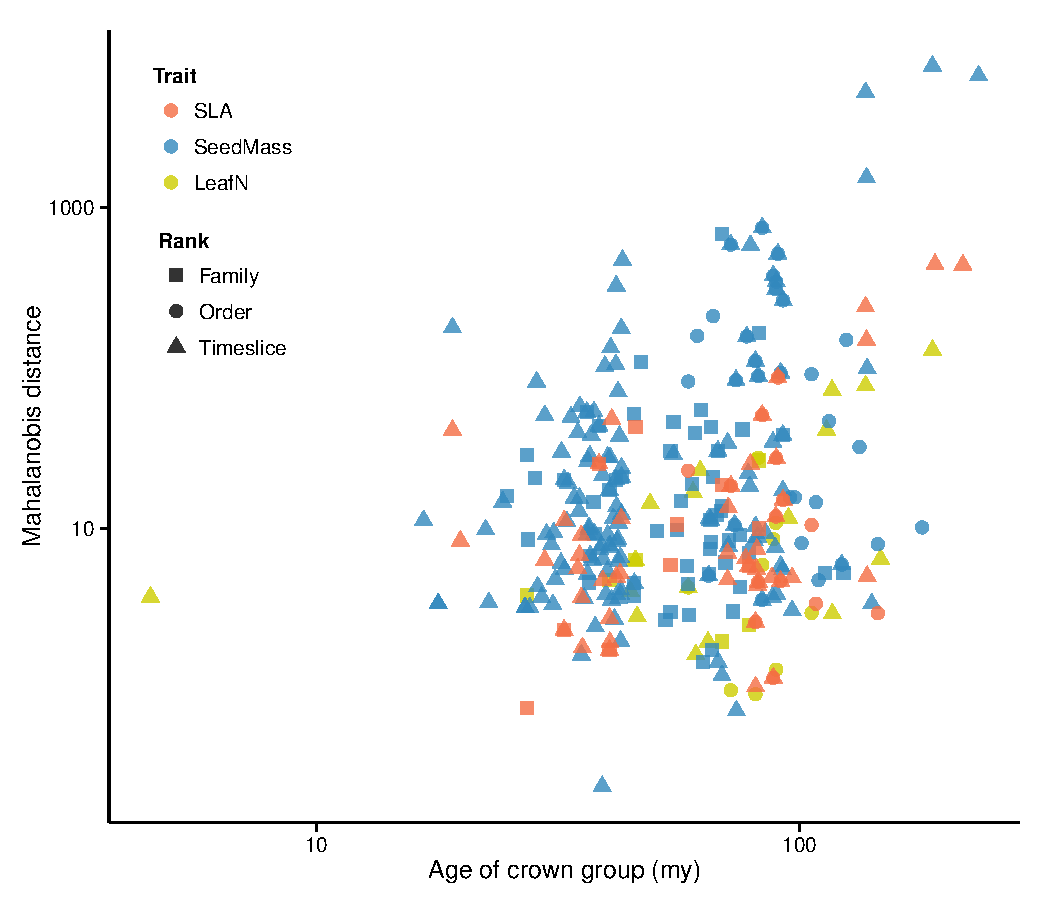
\includegraphics[width=\textwidth]{figs/ad-age-ml}
  \caption[Model adequacy versus clade age (ML)]{The relationship between clade age and a multivariate measure of model adequacy. Considering only the best supported of the three models (as selected by AIC, after fitting the models using ML), there is no  apparent relationship between the age of clade and the distance of the observed and simulated test statistics, as measured by the Mahalanobis distance. Contrast this figure with figure \ref{fig:size-adequacy}, which demonstrates a very tight relationship between clade size and model inadequacy.}
  \label{fig:supp-age-ml}
\end{figure}

Full results from all analyses can be reproduced using code and workflows available at \texttt{https://github.com/richfitz/modeladequacy}. 


\subsubsection{Bayesian Inference}

As with the likelihood results (described in main text), OU models were highly supported across many datasets; 
%% Number of datasets for which OU was best supported model: 177
%% Number of datasets for which OU > 0.75 of DICw: 156
177/337 clades had the highest DIC weight (DIC$_w$) on an OU model; 156 of them with greater than 75\% of the total DIC$_w$ (see figure \ref{fig:supp-dic-support}). While a generally similar pattern of model support holds for both likelihood and Bayesian inference, the likelihood analyses are much cleaner (compare figure \ref{fig:aic-support} and figure \ref{fig:supp-dic-support}). This differnce can be explained by the fact that there is a tight statistical relationship between the AIC values for these three models. If two models have identical likelihoods, the AIC scores, defined as $-2\mathcal{L} + 2k$ (where $\mathcal{L}$ is the log-likelihood of the model and $k$ is the number of parameters) will differ by $2$. As BM is a special case of both OU and EB, in opposite directions in model space, the highest AIC$_w$ possible for BM is $\sim$0.731. The rare clades where both OU and EB have higher support than BM likely reflect problems in optimization. Calculating DIC values from posterior samples is inherently more stochastic; if there is little information in data, the best DIC model will depend on the values sampled by the chain. 

\begin{figure}[p]
  \centering
  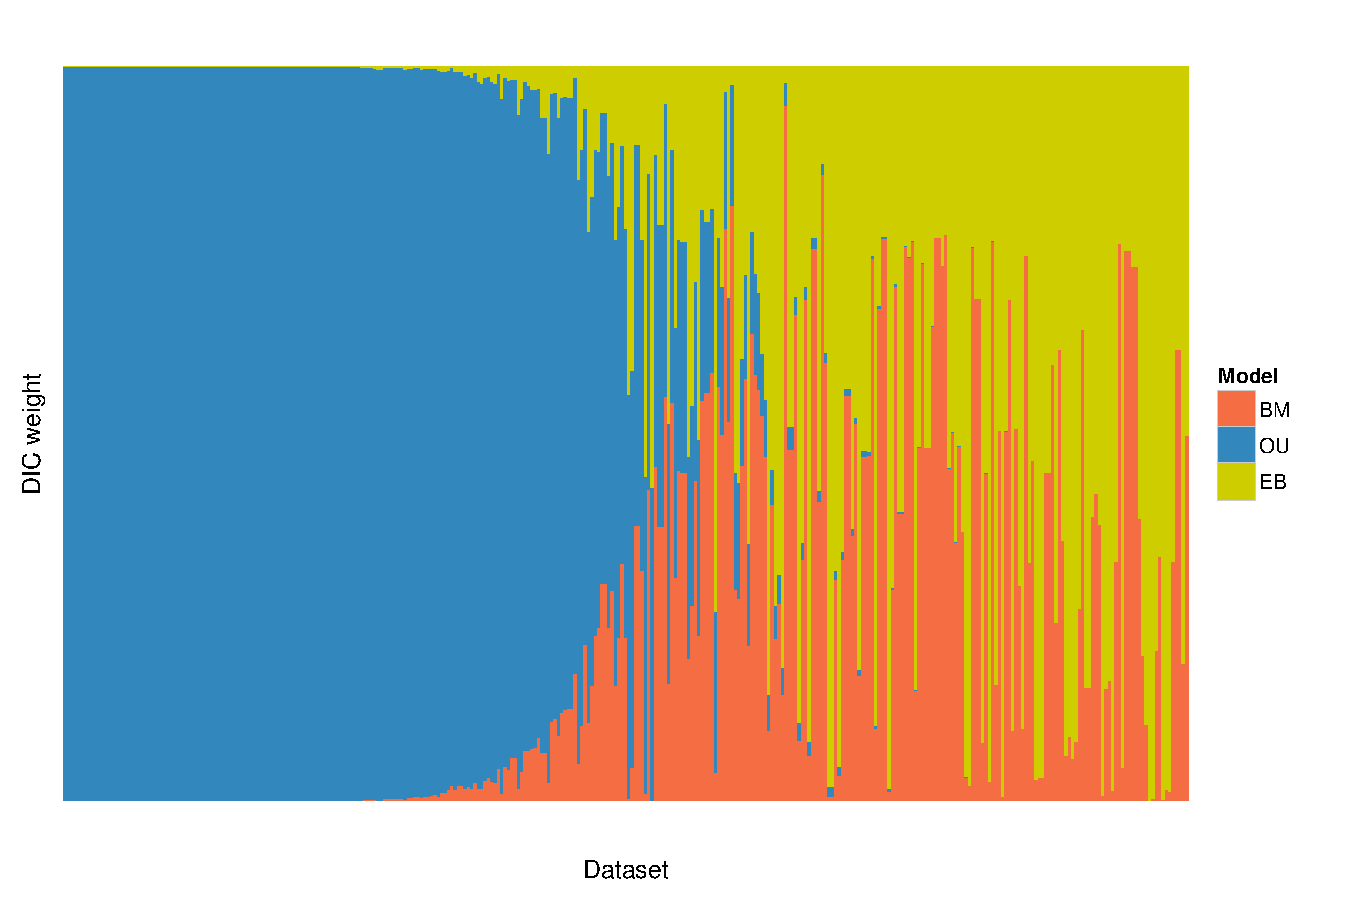
\includegraphics[width=\textwidth]{figs/dic-support}
  \caption[Relative support for models across Angiosperm datasets (Bayesian)]{The relative support, as measured by DIC weight, for the three models used in our study (BM, OU, and EB) across all 337 datasets. All models were fit with MCMC. Like the model comparisons done with AIC, an OU model is highly supported for a majority of the datasets.}
  \label{fig:supp-dic-support}
\end{figure}

For the model adequacy results, the results were also very similar to that of the likelihood analyses (compare to Results section in the main text). The adequacy of these simple models was poor across the majority of the datasets (figure \ref{fig:supp-pvalues}). Again, we limit our analyses of model adequacy to only the most highly supported model in the candidate set.

\begin{figure}[p]
  \centering
  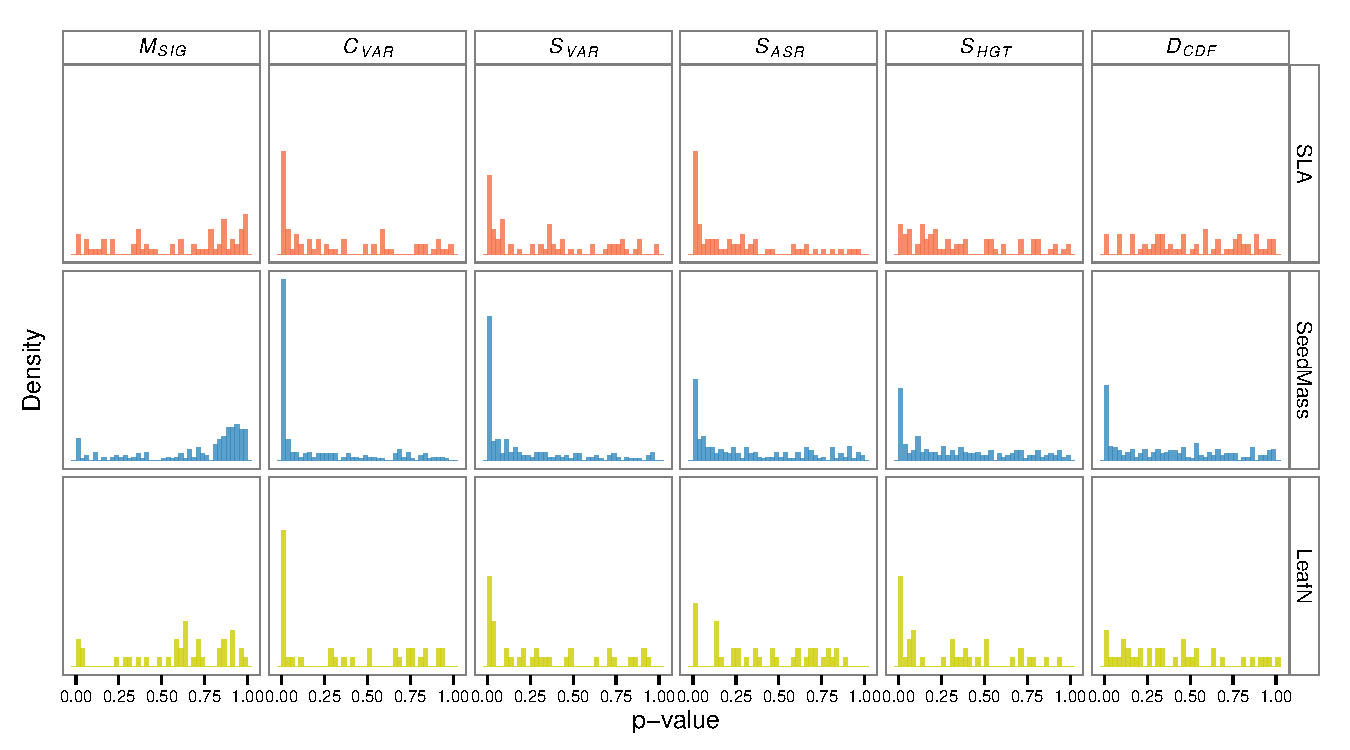
\includegraphics[width=\textwidth]{figs/pval-hist-bayes}
  \caption[Distribution of $p$-values for test statistics (Bayesian)]{The distribution of $p$--values for our six test statistics over all 337 datasets in our study after fitting the models using MCMC. The $p$--values are from applying our model adequacy approach to the best supported of the three models (as evaluated with DIC). Many of the datasets deviate from the expectations under the best model along a variety of axes of variation. Deviations are particularly common for the coefficient of variation $C_{\text{VAR}}$ and the slope of the contrasts against their expected variances $S_{\text{VAR}}$.}
  \label{fig:supp-pvalues}
\end{figure}

%% SLA data 
%% rejected by at least one ss: 35
%% rejected by at least two ss: 26
%% rejected by at least three ss: 19
Of the 72 comparative datasets of SLA, we detected deviations from the expectations of the best supported model using at least one test statistic in 35 cases, 26 by at least two, and 19 by three or more.
%% Seed mass data 
%% rejected by at least one ss: 173
%% rejected by at least two ss: 109
%% rejected by at least three ss: 72
For the seed mass data, we detected deviations with at least one test statistic in 173 cases (by two or more in 109 datasets and by at least three in 72 cases).
%% Leaf nitrogen data
%% rejected by at least one ss: 24
%% rejected by at least two ss: 13
%% rejected by at least three ss: 10
24/39 leaf nitrogen datasets were found to be inadequately described by the best supported model with at least one test statistic (13 by at least two and 10 by at least three).

%% Number rejected by each of the test statistics
%% m.sig: 24
%% c.var: 171
%% s.var: 141
%% s.asr: 101
%% s.hgt: 78
%% d.cdf: 67
Also, similar to the likelihood analyses, the frequency at which deviations were found differed between the test statistics. In 171 cases, we detected model misspecification with $C_{\text{VAR}}$ and with $S_{\text{VAR}}$, 141 ($M_{\text{SIG}}$: 24, $S_{\text{ASR}}$: 101, $S_{\text{HGT}}$: 78, $D_{\text{CDF}}$: 67). Again, only 105 datasets were adequately modeled by one of the three models in our candidate set. There was a strong relationship between model (in)adequacy and clade size (figure \ref{fig:supp-size-adequacy}), but less so for clade age (figure \ref{fig:supp-age-bayes}).

\begin{figure}[p]
  \centering
  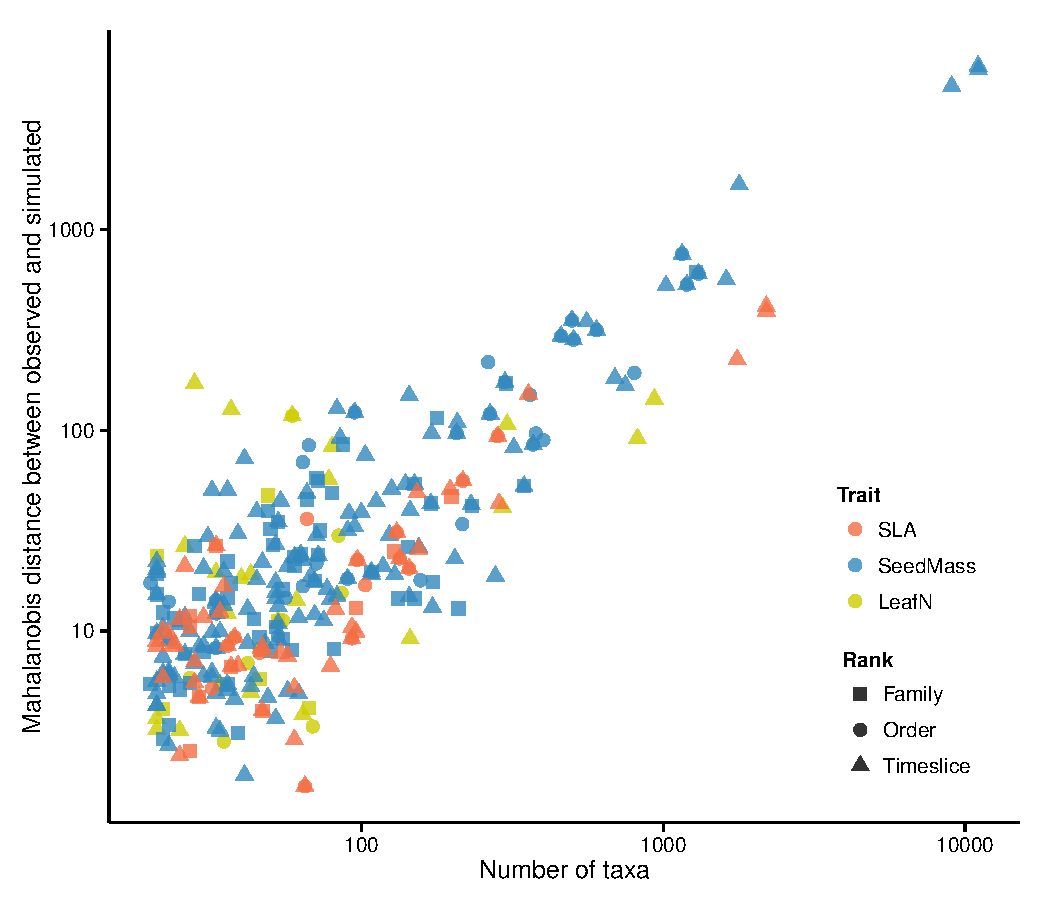
\includegraphics[width=\textwidth]{figs/ad-size-bayes}
  \caption[Model adequacy versus clade size (Bayesian)]{The relationship between clade size and a multivariate measure of model adequacy from the Bayesian analysis. The Mahalanobis distance is a scale--invariant metric that measures the distance between the observed and simulated test statistics, taking into account the covariance between test statistics. The greater the Mahalanobis distance, the worse the model captures variation in the data. Considering only the best supported model for each clade (as chosen by DIC), there is a striking relationship between the two --- the larger the dataset, the worse the models performed (note the logarithmic scale). If the models were equally likely to be adequate at all scales, we would expect no relationship.}
  \label{fig:supp-size-adequacy}
\end{figure}

\begin{figure}[p]
  \centering
  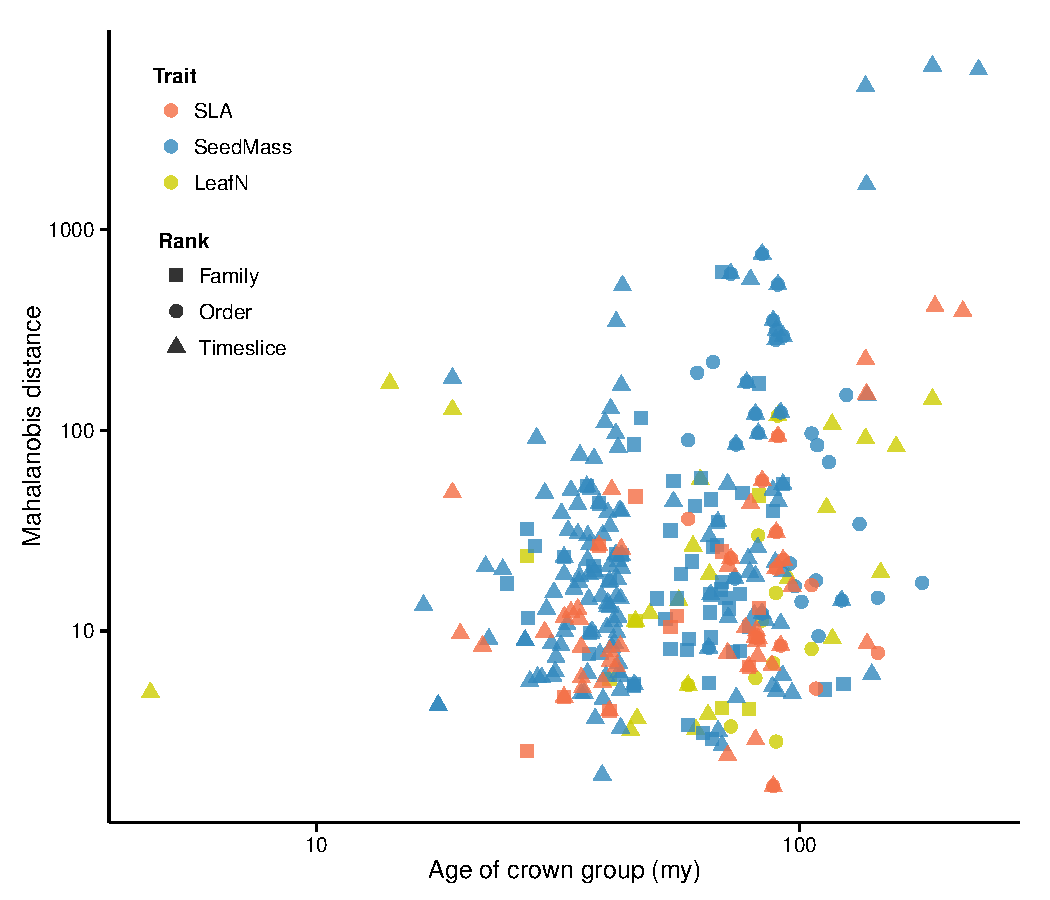
\includegraphics[width=\textwidth]{figs/ad-age-bayes}
  \caption[Model adequacy versus model support (Bayesian)]{The relationship between clade age and a multivariate measure of model adequacy. Considering only the best supported of the three models (as selected by AIC, after fitting the models using MCMC), there is no  apparent relationship between the age of clade and the distance of the observed and simulated test statistics, as measured by the Mahalanobis distance. Contrast this figure with figure \ref{fig:supp-size-adequacy}, which demonstrates a very tight relationship between clade size and model inadequacy.}
  \label{fig:supp-age-bayes}
\end{figure}

\section{Discussion}

\subsection{Why does model adequacy matter?}

Whatever inferences we want to make from comparative data--e.g., characterizing broad-scale patterns of evolution through time, investigating correlations between characters or testing hypotheses about the processes that have driven trait evolution over macroevolutionary time--it is important that our chosen statistical model captures variation in the data \emph{relevant to the question being addressed}. If, for example, the goal is to assess variation in macroevolutionary rates over time, it is essential that the model does a good job of explaning temporally heterogeneity. If we want to know about the slope of an evolutionary allometric relationship, we need a model that provides a meaningful estimate of this parameter \citep{Hansen2012SysBio}. Comparing the fit of a model to a set of alternatives (using likelihood ratio tests, Information Theoretic metrics, Bayes Factors, etc.) can only allow for a relative assessment of the suitability of the model for the task. Such a model comparison approach does not provide any information about whether a model will allow us to actually get at the question we are interested in. 

The flipside of this is that tests of model adequacy, such as ours, are designed to measure the absolute fit but not the absolute appropriateness of the model. We know that all of the models used in comparative biology are wrong. Whether they are useful or not will depend on the question being addressed. We are far from the first to suggest that model adequacy is important to consider when using comparative methods \citep[see, for example][]{Felsenstein1985, Felsenstein1988, HarveyPagel1991, Garland1992, Diaz1996, HansenMartins1996, Price1997, Garland1999, GarlandIves2000, HansenOrzack2005, Hansen2012SysBio, Felsenstein2012, Boettiger2012, SlaterPennell, Beaulieu2013, Blackmon2014}. The contribution of our paper is to generalize many of these previous approaches into a single, flexible statistical framework. 

Again, we emphasize that simply because a dataset deviates from the expectations of the model does not imply that the model should necessarily be rejected. In our analyses of model adequacy across the 337 Angiosperm clades, we were focused on whether the model was suitable for measuring rates of evolution, which is dependent on the model being a good one \citep{Hunt2012}. For other questions, the fact that a model fails to capture some aspects of the variation in the data may not be that important. For example, if our question was that of \citet{Harmon2010}--are early bursts of evolution common in macroevolution?--we could conclude with good certainty that they are not. Our datasets may not be well described by an OU model, but they are certainly nothing like what we would expect under an early burst scenario. Likewise, if we are interested primarily in whether there is a pattern of correlation between two traits, the fact that the model we used is not adequately describing much of the variation will in many cases, not greatly impact the qualitative conclusions.

However, we view the most interesting cases to be where the best model does not adequately describe the variation of interest. The way in which a model fails can provide a richer understanding of our data and the processes that have driven the patterns we observe \citep{Gelman2012}. First, model inadequacy can point to problems in the data. We suspect that this is likely a common cause of poor model fit. For the empirical analyses, we used a very large phylogeny of Angiosperms that was constructed to test specific global-scale biodiversity questions \citep{Zanne2013}. We recognize that the tree is poorly resolved in many places (particularly, near the tips) and is likely ill-suited for addressing more detailed, clade-specific questions \citep[see the recent critique by][]{DonoghueEdwards}. Specifically, the inaccurate placement of species will, on average, cause evolutionary rates to be inflated, which is precisely what we find (see below). However, we emphasize that phylogenetic error is likely ubiquitous and this problem is certainly not limited to the tree we used. Likewise, the dataset we assembled is rather heterogeneous in terms of quality; the data was originally collected for a diverse set of reasons and some groups have been measured much more carefully than others. And while we have done our best to clean the data, errors undoubtedly remain. 

Second, and most excitingly, the failure of a model to adequately describe relevant aspects of the data can provide insight into the processes we have failed to consider in our model \citep{Gelman2012}. For example, if a model fails to capture variation relative to time (evaluated by the test statistic $S_{\text{HGT}}$), this suggests that temporal heterogeneity has been greater than we allowed for. The causes of such heterogeneity have long been a topic of interest in macroevolutionary studies \citep[e.g.,][]{Simpson1944, Foote1997} and there has been a great deal of recent development towards more complex rate-varying models \citep[e.g.,][]{Omeara2006, Thomas2006, Eastman2011, Weir2012, RaboskyBAMM}. Likewise, failure to adequately describe variation across the clade may indicate that the existence of multiple macroevolutionary optima \citep[sensu][]{Hansen2012book} are driving the dynamics of traits over time \citep[see][for models that have been used to capture these dynamics]{Hansen1997, ButlerKing2004, Beaulieu2012, IngramMahler2013, UyedaBayou}. 

Model inadequacy may also suggest types of models that have not previously been considered. For example, if recently diverged species tend to more dissimilar than can be accounted for under a simple diffusion model such as BM or OU, this may be the result of character displacement. However, almost no phylogenetic models have been put forth that explicitly model interactions between lineages \citep[but see][]{NuismerHarmon}. Or if traits have lower variance than expected under an OU process, this may be the result of hard bounds. \citet{Davies2014} recently argued that this is the case for climatic niches and that alternative models need to be developed for this case. Of course, a researcher may discover that her dataset is poorly described by all of the currently available models. Aside from deriving new models specific to her question and dataset, she should at least carefully examine the extent to which model misspecification is likely to affect the major conclusions and proceed forward with due caution.
 
\subsection{Implications for empirical studies}

In our analysis of Angiosperm functional traits, we found common macroevolutionary models to often be poor descriptors for the patterns of variation and likely inadequate for estimating evolutionary rates. While there are certainly a number of important caveats to our analysis (discussed above), the overall trends are clear. This should certainly give researchers some pause about the models routinely used in our field--especially as they are often used in a model comparison framework to evaluate the ``tempo and mode'' of macroevolution. We argue that our results strongly suggest that we may often be missing a large part of the story.

The 337 comparative datasets we analyzed varied in terms of traits, size, age and placement in the Angiosperm phylogeny. Nonetheless, several general patterns emerge. An OU model, was by and large, the most supported of the three we examined. In an analysis of 67 comparative datasets consisting of size and shape data from a variety of animal taxa, Harmon et al. \citep{Harmon2010} also found substantial support for OU models, though for their datasets, BM was more commonly chosen by AIC. \citep[We note, however, that many of their datasets were quite small; see][]{SlaterPennell}. Since their paper, a substantial number of studies conducted in a diverse array of groups have also found OU models to be preferred over BM models \citep[e.g.,][]{Burbrink2012, Wiens2013, Lopez2013, Thomaspreprint}. 

The tendency of OU to explain data better than BM has inspired diverse process-based explanations, including stabilizing selection, evolutionary constraints and the presence of ``adaptive zones'' \citep{HansenMartins1996, ButlerKing2004, Hansen2012book, PennellHarmon}. 
If the widespread support for OU models was indeed caused by the biological processes that have been proposed, we would expect that an OU model would also be widely adequate. However, this is not what we found. The datasets deviated significantly from the distributions expected under OU models, most often detected with $C_{\text{VAR}}$ and $S_{\text{VAR}}$ but frequently with others as well. OU models often failed to capture other important types of heterogeneity-variation with respect to rate variation ($M_{\text{SIG}}$), trait values ($S_{\text{ASR}}$) and time ($S_{\text{HGT}}$). Additionally, a substantial number of datasets were not well-modeled by a multivariate normal distribution ($D_{\text{CDF}}$). These results suggest a statistical explanation for the high support for OU models. OU predicts higher variance near the tips of the phylogeny than do BM or EB models \citep[see figure 1 in][]{Harmon2010}. 
Heterogeneous evolutionary processes, phylogenetic misestimation and measurement error could also produce such a pattern. In light of our results from model adequacy, it seems likely that OU is often supported because it is able to accommodate more ``slop'' (phylogenetic and trait error in addition to model misspecification) than the other models.  This is not to say that the processes captured by OU models are unimportant in macroevolution, but rather that OU models may be favored for reasons that are more statistical than biological. Future, and hopefully more widely adequate, models of trait evolution could be developed that both include aspects of the OU model, especially the bounds on trait values, while incorporating additional biological realism \citep[for a recent example of such a model, see][]{NuismerHarmon}.

The way in which the observed test statistics deviate from the simulated values also supports the claim that the widespread support for OU is largely a statistical artifact. Model violations were most frequently detected by the variance estimate, $C_{\text{VAR}}$. If the evolutionary process (or, alternatively, phylogenetic/measurement error) is heterogeneous across the tree, the lineages in some parts of the clade will be much more divergent than in others. The only way for the model to account for the highly divergent groups is to estimate a large $\sigma^2$ (and/or a small $\alpha$ parameter for the OU model). The unit tree formed by these parameter estimates will have long branches across the entire tree. In the less divergent parts of the tree, the contrasts calculated on this unit tree will be small, relative to what we expect under BM. So perhaps counter-intuitively, when heterogeneity in processes across taxa cause the estimated global rates of divergence to be inflated, resulting in a higher value for $C_{\text{VAR}}$.

The second major take-home from the empirical analyses is that error, both in trait values and phylogenies, can have serious consequences for model adequacy. We frequently detected deviations from model expectations with $S_{\text{VAR}}$, the slope between the contrasts and their expected variances. This is indicative the rate of evolution appears to be varying with regards to branch length over which it is measured. This seems unlikely to be attributable to any biological process; it is far more probable that this reflects phylogenetic error (particularly, branch length error). Above, we outlined some of the deficiencies of the datasets we used in this paper but argue that these are likely to be widespread in comparative data. The test statistics outlined above can serve as useful diagnostics to aid researchers in identifying outliers that may be driving the pattern. We recommend that researchers faced with an inadequate model plot the magnitude of the contrasts on to the unit tree; this will usually be much more informative with regards to the model fit than plotting the magnitude of the contrasts on the original phylogeny. Exceptionally large or small contrasts on the unit tree can provide clues as to where the data may be erroneous. If phylogenetic error were causing poor model fits, we would predict that many of the anomalous contrasts would occur in parts of the tree that are poorly supported.
 
\subsection{Extensions of our approach}

There are a number of additional ways our approach could be extended. First, we have only considered a limited set of test statistics. We chose them because each of these has a clear statistical expectation and observed deviations from them have intuitive biological explanations. However, they are certainly a subset of all possible test statistics that could be applied. 
For example, because contrasts are i.i.d., there should be no autocorrelation between neighboring contrasts; the test statistics could be expanded to detect non-zero autocorrelation. Second, as stated above, our approach can be applied equally well to phylogenetic regression models, such as phylogenetic generalized least squares \citep{Grafen1989, MartinsHansen1997} or phylogenetic mixed models \citep{Lynch1991, Housworth2004, Hadfield2010}, where concerns regarding model adequacy are just as pertinent \citep{Hansen2012SysBio}. While our approach can be used to assess the adequacy of the phylogenetic component of regression models ``out of the box'', additional steps are required to assess the adequacy of the linear component.  Third, our method was designed for quantitative trait models that assume data can be modeled with a multivariate normal distribution. We need general model adequacy approaches for other types of traits, such as: discrete traits \citep[i.e., binary, multistate, ordinal; see][for recent discussions of this]{Beaulieu2013, Blackmon2014, MaddisonFitzJohn}; traits that influence speciation rates \citep[e.g.,][]{Maddison2007, FitzJohn2010} and quantitative trait models that do not predict a multivariate normal distribution of traits \citep{Landis2012, Landispreprint}.

It may also be possible to extend our approach with an eye towards model selection. \citet{SlaterPennell} developed their posterior predictive simulation approach (which is related to our method) to distinguish between a BM model and one where rates of evolution decreased through time. They chose test statistics specifically to address this question. Slater and Pennell found using posterior predictive fit as a model selection criterion to be much more powerful than comparing models using AIC or likelihood ratio tests, particularly when ``outlier taxa'' (lineages where the pattern of evolution deviates from the overall model) were included in the analysis. The logic of Slater and Pennell could be extended to other scenarios; to test some evolutionary hypotheses, we may care a lot about whether a model explains varation along some axes but be less concerned about others. This is a question-specific approach to model selection and has been developed in the context of molecular phylogenetics \citep{Bollback2002, Lewis2013}. This is also the essence of the Decision-Theoretic approach to model selection \citep{Robert2007}, which has also been well-used in phylogenetics \citep{Minin2003}, but has not previously been considered in PCMs.


\section{Arbutus}

We have implemented our approach in a new R package \textsc{arbutus}. It is available on github \texttt{https://github.com/mwpennell/arbutus}. For this project, we have also adopted code from the \textsc{ape} \citep{ape}, \textsc{geiger} \citep{geiger2} and \textsc{diversitree} \citep{FitzJohn2012} libraries. We have written functions to parse the output of a number of different programs for fitting trait evolution models (see the \textsc{arbutus} website for an up-to-date list of supported models and packages). As this approach was developed to be general, we have written the code in such a way that users can include their own test statistics and trait models in the analyses.

\section{Concluding remarks}
Attempts to assess the adequacy of phylogenetic models are almost as old as modern comparative phylogenetic biology. In the 1980s and 1990s much discussion surrounded the appropriateness of various methods and models \citep{Felsenstein1985, Felsenstein1988, HarveyPagel1991, Garland1992, Diaz1996, Price1997, Garland1999, GarlandIves2000}. We argue that this discussion is key to progressing in our field. This is not simply because we are concerned that many inferences may not be robust to model violations. Rather, we believe that considering model adequacy can help suggest new ways of thinking about how to combine data and models to test macroevolutionary hypotheses.

\chapter[How much of the world is woody? Dealing with sampling error in comparative data]{How much of the world is woody? Dealing with sampling error in comparative data\footnote {Previously published as: FitzJohn, R.G., M.W. Pennell, A.E. Zanne, P.F. Stevens, D.C. Tank, and
  W.K. Cornwell. 2014. How much of the world is woody? 
  Journal of Ecology 102:1266--1272.}}
\label{chap:wood}

\section{Summary}
The question posed by the title of this paper is a basic one,
  and it is surprising that the answer is not known. Recently
  assembled trait datasets provide an opportunity to address this, but
  scaling these datasets to the global scale is challenging because of
  sampling bias.  Although we currently know the growth form of tens
  of thousands of species, these data are not a random sample of
  global diversity; some clades are exhaustively characterised, while
  others we know little-to-nothing about.Starting with a database of woodiness for 39,313 species of
  vascular plants (12\% of taxonomically resolved species, 59\% of
  which were woody), we estimated the status of the remaining
  taxonomically resolved species by randomisation.  To compare the
  results of our method to conventional wisdom, we informally surveyed
  a broad community of biologists.  No consensus answer to the
  question existed, with estimates ranging from 1\% to 90\% (mean:
  31.7\%).After accounting for sampling bias, we estimated the proportion
  of woodiness among the world's vascular plants to be between 45\%
  and 48\%.  This was much lower than a simple mean of our dataset and
  much higher than the conventional wisdom. Alongside an understanding of global taxonomic
  diversity (i.e., number of species globally), building a functional
  understanding of global diversity is an important emerging research
  direction.  This approach represents a novel way to account for
  sampling bias in functional trait datasets and to answer basic
  questions about functional diversity at a global scale.

\section{Introduction}

The distinction between a woody and non-woody growth-form is
probably the most profound contrast among terrestrial plants and
ecosystems: for instance, a forest is dominated by woody taxa 
while a grassland is dominated by herbs.  The recognition of the fundamental
importance of this divide dates back at least to \textit{Enquiry into
  Plants} by Theophrastus of Eresus (371-287 BC), a student of
Plato and Aristotle, who began his investigation into plant form and
function by classifying the hundreds of plants in his garden into
woody and herbaceous categories \citep{theophrastus1916enquiry}.

The last two thousand years of research into wood since Theophrastus
classified his garden have uncovered its origin in the early Devonian
($\sim$400 Mya; \citealt{gerrienne2011simple}); that prevalence of
woodiness varies with climate \citep{Molesheihgt}; that wood has been
lost many times in diverse groups, both extant and extinct
\citep{judd1994}, often as an adaptation to freezing temperatures
\citep{Zanne}; that it has also been gained many times,
particularly on island systems \citep{Carlquist1974,Givnish1998};
and that many different forms of pseudo-woody growth
habit have appeared across groups that have lost true woodiness or
diverged before true woodiness evolved \citep{Cornwellwood}.  We know
about its mechanical properties and developmental pathways, its
patterns of decomposition and their effects on ecosystem function
\citep{Cornwellwood}, and that woody and herbaceous species have
markedly different rates of molecular evolution \citep{SmithDonoghue}.
%
However, we have no idea about what proportion of species in the world
are actually woody.

Recently assembled functional trait datasets provide an opportunity to
address this question. However, such datasets are, almost without
exception, biased samples of global diversity.  Researchers collect
data for specific questions on a local scale, and assembling these
local datasets creates a useful resource \citep{kattge2011try}.  But
as with GenBank's assembly of genetic data
\citep{smith2011understanding}, the simple compilation of data is not
an unbiased sample, and these initial sampling biases will, in turn,
bias downstream analyses.  Understanding and accounting for the biases
in these datasets is an important and necessary next step.

We sought to develop an approach that accounts for this bias.  In
doing so, we were able to re-ask Theophrastus' 2000-year old
question at a global scale: how many of the world's plant species are
woody?
%
We also sought to understand how well scientists were able to overcome
this bias and make a reasonable estimate.  To do this, we took the
unconventional approach of coupling our analysis with an informal
survey in which we asked our question to the broader community of
botanists and other biologists.

\section{Materials and methods}

\subsection{Dataset}

We used a recently assembled database with growth-form data for
49,061 vascular plant species (i.e., lycopods, ferns, gymnosperms and
angiosperms), which is the largest such database assembled to date
\citep[][available on the Dryad data repository;]{ZanneDryad,Zanne}.
%
This database uses a functional definition of woodiness: woody species
have a prominent above-ground stem that persists through time and changing
environmental conditions and herbaceous species lack such a 
stem--a definition originally suggested by Asa Gray \citeyearpar{gray1887elements}. 
\citet{Zanne}
chose this simple definition because it best characterised the functional
aspect of growth form that they investigated, allowing them to compare 
species that maintain an above-ground stem through freezing conditions to 
ephemeral species that avoid freezing conditions.  More precise definitions 
that rely on lignin content and/or secondary vascular tissue from a bifacial
cambium are problematic because there are many exceptions depending on tissue 
type, times of development, or environmental conditions 
\citep{Groover2005, Spicer2010, Rowe2012}.  
Because our analyses and survey were based on this database, 
we present this functional definition of woodiness here for clarity 
(see \citet{Zanne} for a discussion of the various definitions of woodiness, 
their merits, and pitfalls).  Note that in addition to species producing
secondary xylem, this definition
classifies, among other groups, palms, tree ferns and bamboo as
woody.

As with all large data assemblies, the underlying datasets were collected 
for a variety of research goals. For example, a number of the datasets come
from forestry inventories, which, of course, are biased towards recording
woody species. Other sources of sampling bias, including geographically restricted sampling 
in many sub-datasets, may be less obvious but
nonetheless may have major implications for the inferences drawn from 
aggregate databases.

Because the effort to organise plant taxonomy, especially synonymy, is
on-going, there was uncertainty regarding the status of many plant
names.
%
To bring species binomials to a common taxonomy among datasets, names
were matched against accepted names in the Plant List
\citep{ThePlantList}.  Any binomials not found in this list were
matched against the International Plant Name Index
(\url{http://www.ipni.org/}) and Tropicos (\url{http://www.tropicos.org/}).
Potential synonymy in binomials arising from the three lists was
investigated using the Plant List tools \citep{ThePlantList}.  
% NOTE: This is the cleaning step done by `load.woodiness()`.
As a result of this cleaning, the number of species in the final
dataset was reduced from 49,061 to 39,313.
% #rstats
% nrow(read.csv("data/zae/GlobalWoodinessDatabase.csv")) # 49061
% nrow(load.woodiness())                                 # 39313

Theophrastus recognised both the fundamental importance of the
distinction between woody and herbaceous plants, and that this
distinction is in some cases difficult to make.  There are two ways
that species were recorded as ``variable'' in form
\citep{Beaulieu2013}.  First, different records of a single
species may conflict in growth form (having both records of woodiness
and herbaceousness); this affected 307 of the 39,313 species in the
database.
% #rstats
% dat <- load.woodiness()
% tmp <- parse.count(dat$woodiness.count)
% multi <- rowSums(tmp > 0) > 1
% sum(multi)        # 307
% nrow(tmp)         # 39313
% mean(multi) * 100 # 0.8%
Second, 546 species (1.4\%) were coded as variable.
% #rstats
% sum(tmp[,"V"] > 0)  # 546
% nrow(tmp)           # 39313
% mean(tmp[,"V"] > 0) # 0.014
% sum(tmp[,"V"] > 0 & rowSums(tmp[,c("H", "W")]) > 0) # 53 (of 546)
Following \citet{Beaulieu2013}, we coded species in these
groups as ``woody'' or ``herbaceous'' when a majority of records were
either ``woody'' or ``herbaceous'', respectively, and for these
species, records of ``variable'' do not contribute to the analysis.
%
%
Our final database for the main analysis contained 38,810 records with
both information on woodiness and documented taxonomy--15,957 herbs
and 22,853 woody species.  
% #rstats
% sum(dat.g$K) # 38810 - known species
% sum(dat.g$H) # 15957 - herbs
% sum(dat.g$W) # 22853 - woody species
This included records from all flowering plant orders currently
accepted by APG III \citep{APG3} and the fern taxonomy of
\citet{apweb}, covering 15,232 genera and 465 families.
% #rstats
% sapply(dat.g[c("genus", "family")], function(x) length(unique(x)))
The 503 species excluded at this step had identical numbers of records
of being woody and herbaceous.
% #rstats
% nrow(dat) - sum(dat.g$K)    # 503
% sum(tmp[,"W"] == tmp[,"H"]) # 503
We also ran analyses where we coded growth forms by treating species
with \emph{any} record of woody or variable as ``woody'' (and
similarly for herbaceous), using all 39,313 species.  Neither of these
cases are likely to be biologically realistic but allowed us to
evaluate the maximal possible effect of mis-coding variable species.

\subsection{Estimating the percentage of species that are woody}

To estimate the percentage of species that are woody, we cannot simply
use the fraction of species within our trait database that are woody
(22,853 of 38,810 = 59\%) as these records represent a biased sample
of vascular plants.
% #rstats
% sum(dat.g$W) # 22853 - woody
% sum(dat.g$K) # 38810 - known
% sum(dat.g$W) / sum(dat.g$K) # 0.59 - fraction
For example, most Orchidaceae are probably herbaceous; we have only
one record of woodiness among the 1,537 species for which we have
data.
% #rstats
% i.orc <- dat.g$family == "Orchidaceae"
% sum(dat.g$K[i.orc]) # 1537 - known Orchidaceae
% sum(dat.g$W[i.orc]) # 1    - woody Orchidaceae
However, the fraction of Orchidaceae species with known data (1,537 of
27,801 = 6\%)
% sum(dat.g$K[i.orc]) #  1537 - known Orchidaceae
% sum(dat.g$N[i.orc]) # 27801 - number of Orchidaceae
% sum(dat.g$K[i.orc]) / sum(dat.g$N[i.orc]) # 0.055 - fraction known
is much lower than the overall rate of knowledge for all vascular
plants (38,810 of 316,143 = 12\%), which will upwardly bias the global
estimate of woodiness.
% #rstats
% sum(dat.g$K) #  38810 - known vascular
% sum(dat.g$N) # 316143 - total vascular
% sum(dat.g$K) / sum(dat.g$N) # 0.12 - fraction known
Conversely, systematic under-sampling of tropical species would bias
the global woodiness estimate downwards, as tropical floras are
thought to harbour a greater proportion of woody species than
temperate ones \citep{Molesheihgt}.

We developed a simple method to account for this sampling bias when
estimating the percentage of woody species.  In our approach, we treat
each genus separately, and in all cases know that there are are $n_w$
woody and $n_h$ herbaceous species and a total of $N$ species in the genus.
%
For example, the genus \textit{Microcoelia} (Orchidaceae) has 30
species in total, and we know that 12 are herbaceous and none are
known to be woody ($N = 30$, $n_w = 0$, $n_h = 12$). We do not know
the state of the remaining 18 species, so the true number of woody
species, $N_w$, must lie between 0 and 18. In general, we cannot
assume that these species are all herbaceous, even though both
biological and mathematical intuition suggest that most of them will
be.
% #rstats
% i.mic <- which(dat.g$genus == "Microcoelia")
% dat.g[i.mic,c("N", "W", "H")]   # 30, 0, 12
% dat.g$N[i.mic] - dat.g$K[i.mic] # 18

We used two different approaches for imputing the values of these
unknown species. First, we assumed that the known species were sampled
without replacement from a pool of species with $N_w$ woody and $N_h$
herbaceous species ($N_w + N_h = N$), following a hypergeometric
distribution. The probability that $x$ of the species of unknown state
are woody ($x = 0, 1, \ldots, N - n_w - n_h$) is proportional to
\begin{equation}
  \Pr(N_w = x) \propto {n_w + x \choose n_w}
  {N - n_w - x \choose n_h}
\end{equation}
Under this sampling model, the more species for which we do not have data,
the greater the uncertainty in our estimates for the proportion of species
which are woody.
%
For \textit{Microcoelia} this model gives a 42\% probability that all
species are herbaceous, and a 90\% chance that at most 3 species
are woody.
% #rstats
% # Based on the code inside rhyper2()
% n <- dat.g$N[i.mic]; w <- dat.g$W[i.mic]; h <- dat.g$H[i.mic]
% xw <- seq(w, n - h) # possible number of woody species
% xh <- n - xw
% ph <- dhyper(h, xh, xw, h + w) # probability of (xh[i], xw[i])
% ph <- ph / sum(ph) # normalise
% ph[1]        # 0.42 - all species herbaceous
% sum(ph[1:4]) # 0.90 - at most 3 species woody
This approach probably overestimates the number of woody species in
this case, and in other cases where all known species are woody (e.g.,
\textit{Actinidia} [Ericaceae]) it will probably underestimate the
number of species that are woody. We see this as corresponding to a
weak prior on the shape of the distribution of the fraction of woody
species within a genus and will refer to this as the ``weak prior''
approach because it weakly constrains the state of missing species.

However, the distribution of woodiness among genera and families is
strongly bimodal; most genera are either all-woody or all-herbaceous
(Fig. \ref{fig:distribution-genera}, Fig. \ref{fig:distribution-family}, and 
\citealt{sinnott1915evolution}).  Among the 791 genera with at least 10
records, 411 are entirely woody, 271 are entirely herbaceous, and only
58 have between 10\% and 90\% woody species. Qualitatively similar patterns
hold at both the level of family and order, though the distribution
becomes progressively less bimodal as one moves up the taxonomic hierarchy 
(Figs. \ref{fig:distribution-family} and \ref{fig:distribution-order}). 
As a result, knowing the state of a handful of species within a genus 
can give a reasonable guess at the state of remaining species.
% #rstats
% tmp <- dat.g$p[dat.g$K >= 10] # select genera with 10 records
% length(tmp)              # 791 - genera with at least 10 records
% sum(tmp == 1)            # 411 - 100% woody
% sum(tmp == 0)            # 271 - 100% herbaceous
% sum(tmp > 0 & tmp < 1)   # 109 - variable
% sum(tmp > .1 & tmp < .9) #  58 - interestingly variable

\begin{figure}[p]
  \centering
  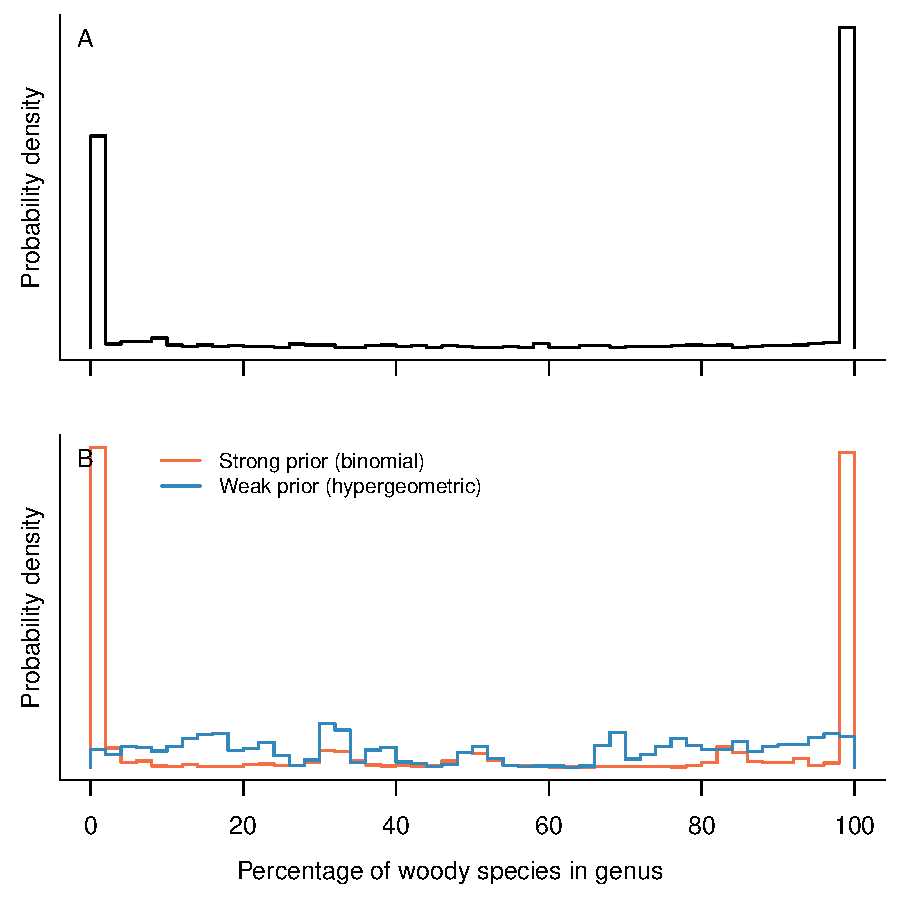
\includegraphics[width=\textwidth]{figs/fraction-by-genus}
  \caption[Distribution of woodiness proportion among genera]{Distribution of the percentage of woodiness among genera.
    The distribution of the percentage of species that are woody within
    a genus is strongly bimodal among genera (panel A--showing
    genera with at least 10 species only).
    % 
    The two different sampling approaches generate distributions that
    differ in their bimodality (panel B). If we sample species
    with replacement from some pool, with a weak prior on
    the fraction of woodiness within the pool, then we generate a broad
    distribution with many polymorphic genera (blue line).
    Sampling with replacement, assuming that species are drawn from a
    pool of species that has a fraction of woody species equal to the
    observed fraction of woodiness, generates a strongly bimodal
    distribution (red line).}
  \label{fig:distribution-genera}
\end{figure}

\begin{figure}[p]
  \centering
  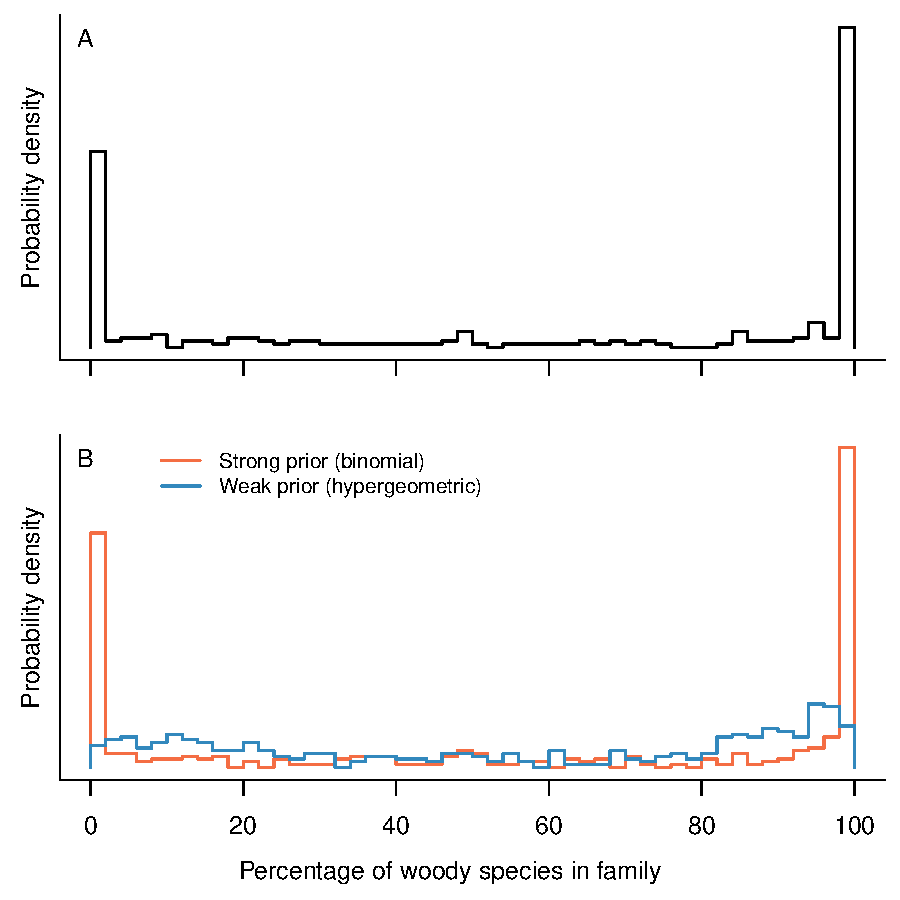
\includegraphics[width=\textwidth]{figs/fraction-by-family}
  \caption[Distribution of woodiness proportion among
  families]{Distribution of the percentage of woodiness among
    families.
    The distribution of the percentage of species that are woody within
    a family is strongly bimodal among families (panel A), though less
    strongly bimodal than among genera.
    % 
    The two different sampling approaches generate distributions that
    differ in their bimodality (panel B).  Using the weak prior
    approach generates a broad distribution with many polymorphic
    genera (blue line), while using the strong prior approach
    generates a strongly bimodal distribution (red line).}
  \label{fig:distribution-family}
\end{figure}

\begin{figure}[p]
  \centering
  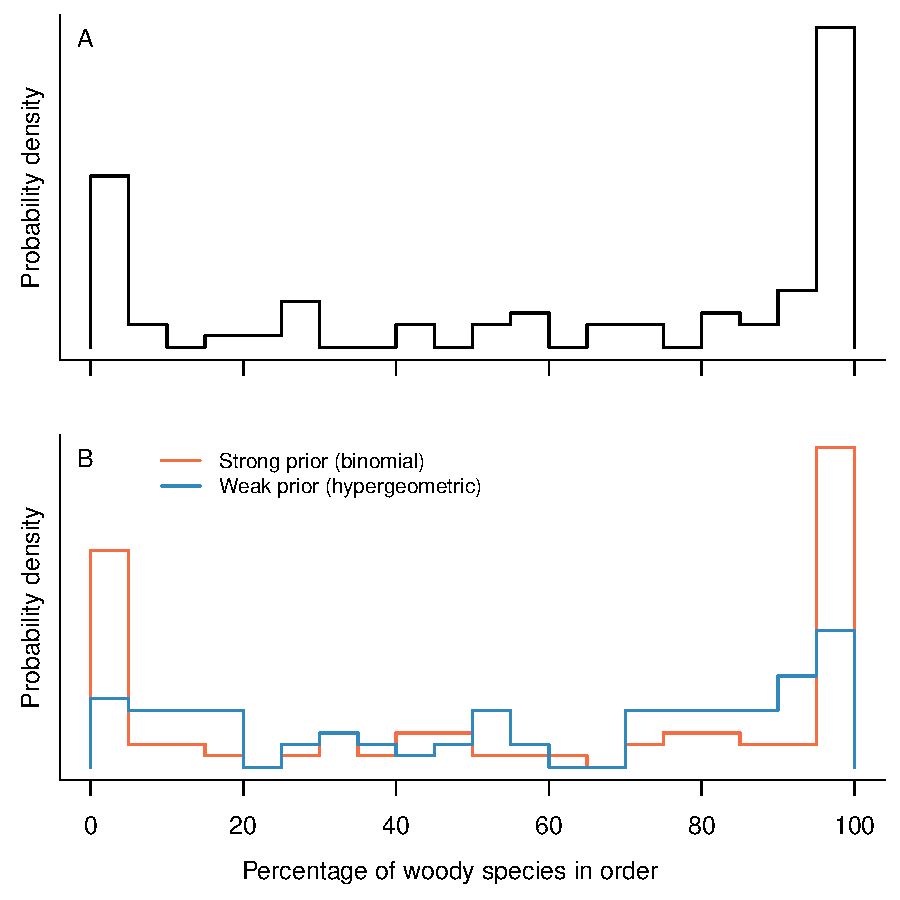
\includegraphics[width=\textwidth]{figs/fraction-by-order}
  \caption[Distribution of woodiness proportion among
  orders]{Distribution of the percentage of woodiness among orders.
    The distribution of the percentage of species that are woody within
    an order is bimodal among orders (panel A), though
    less strongly bimodal than among both genera and families.
    % 
    The two different sampling approaches generate distributions that
    differ in their bimodality (panel B).  Using the weak prior
    approach generates a broad distribution with many polymorphic
    genera (blue line), while using the strong prior approach
    generates a strongly bimodal distribution (red line).}
  \label{fig:distribution-order}
\end{figure}


To model the other extreme of sampling, we used an approach where we
computed the observed fraction of woody species 
\[p_w = n_w / (n_w +n_h)\] 
and sampled the state of the unobserved species using a
binomial distribution, which represents the case of sampling
with replacement. In this case the probability that $x$ of the species
are woody is:
\begin{equation}
  \Pr(x = k) = {N - n_w - n_h \choose k - n_w} 
  p_w^k (1-p_w)^{N - n_h - k}.
\end{equation}
%
In cases where all known species are woody (or herbaceous as in
\textit{Microcoelia}) this will assign all unknown species to be woody
(or herbaceous). For such genera, increasing the number of unobserved
species will not increase the uncertainty in the estimate, in contrast
to the weak prior sampling approach.
%
We therefore see the binomial sampling approach as corresponding to a
very strong prior on the bimodal distribution of woodiness among
genera, and we will refer to this as the ``strong prior'' approach
because it more strongly constrains the state of missing species
within genera with no known polymorphism.  While neither of these
approaches is ``correct'', they probably span the extremes of possible
outcomes.
%
In polymorphic genera the two approaches will give similar results,
especially where the number of unknown species is relatively large.

For genera where there was no information on woodiness for any
species, we sampled a fraction of species that might be woody from
the empirical distribution of woodiness fractions \textit{among
  genera} within the same order. We did this after imputing the
missing species values within those other genera. So, if a genus is
found in an order with genera that had woodiness fractions of $\{0, 0,
0.1, 1\}$ we would have approximately a 50\% chance of sampling a 0\%
woodiness fraction for a genus, with probabilities from 0.1 to 1 being
fairly evenly spread.  Given this woodiness fraction, we then sampled
the number of species that are woody from a binomial distribution with
this fraction and the number of species in the genus as its
parameters.
% #rstats
% hist(quantile(c(0, 0, 0.1, 1), runif(10000)))

In addition to the number of species known to be woody and herbaceous,
we also require an estimate of the number of species per genus.  For this, we
used the number of accepted names within each genus in the Plant List
\citep{ThePlantList}. The taxonomic resources were compiled by \citet{Zanne}
are on available on Dryad \citep{ZanneDryad}.

For each genus, we sampled the states of unobserved species, from
either the hypergeometric or binomial distribution, parametrised from
the observed data for that genus.
%
For each sample we can then combine these estimates to compute the
number (or fraction) of species that are woody at higher taxonomic
levels (family, order or vascular plants).  We repeated this sampling
1,000 times to generate distributions of the number (or fraction) of
species that are woody.
%
The R code and data to replicate this analysis are available on github
(\url{https://github.com/richfitz/wood}).

\subsection{Survey}

In estimating the number of species within Angiosperm families,
\citet{joppa2010} found that expert opinion generally agreed closely
with estimates from a statistical model.  We were interested in
whether a consensus answer existed--even if not formalised in the
literature--and if so, whether it was consistent with our
estimates.
% 
We created an English-language survey (which we also translated into
Portuguese) asking for an estimate of the percentage of species that
are woody according to the above definition.  We also asked
respondents to indicate their level of familiarity with plants, level
of formal training, and the country in which they received their
training. We distributed the survey to the 
community via several electronic
mailing lists with wide circulation among biologists: \textsc{evoldir},
\textsc{ecolog}, \textsc{\mbox{r-sig-phylo}}, \textsc{taxacom},
\textsc{herbaria}, as well as local lists. We also posted links on the
social-networking platforms \textsc{google+}, \textsc{twitter} and
\textsc{facebook} to reach a broad audience.
%
In order to increase representation of survey responses from Latin
America, we translated the survey into Portuguese and distributed it
to Brazilian biology \textsc{facebook} groups and university mailing
lists.

To analyse the survey data, we used linear regression on
logit-transformed percent woodiness as \citep[see][]{wartonarcsine}
and treated the self-reported level of botanical familiarity and
education as factors.  We converted country of training to coarse
latitude using shapefiles
from the \textsc{gbif} dataportal \citep{GBIFdata},
and converted these into ``tropical'' and ``temperate'' using an
absolute latitude of 23$^\circ$~26$^\prime$. 

\section{Results}

Across all vascular plants, we estimated the fraction of woody species
to be between 45\% and 48\%.
% #rstats
% round(100*res.b$overall.p, 1) # 45.5 (45.2 - 45.8)
% round(100*res.h$overall.p, 1) # 47.6 (46.9 - 48.2)
Specifically, using our strong prior sampling approach (binomial
distribution) we estimated 45.6\% of species are woody (95\%
confidence interval of 45.3-45.9\%) and with the weak prior
(hypergeometric distribution) approach we estimated 47.6\% (95\% CI of
46.9-48.2\%) (Fig. \ref{fig:distribution-raw}).
%

\begin{figure}[p]
  \centering
  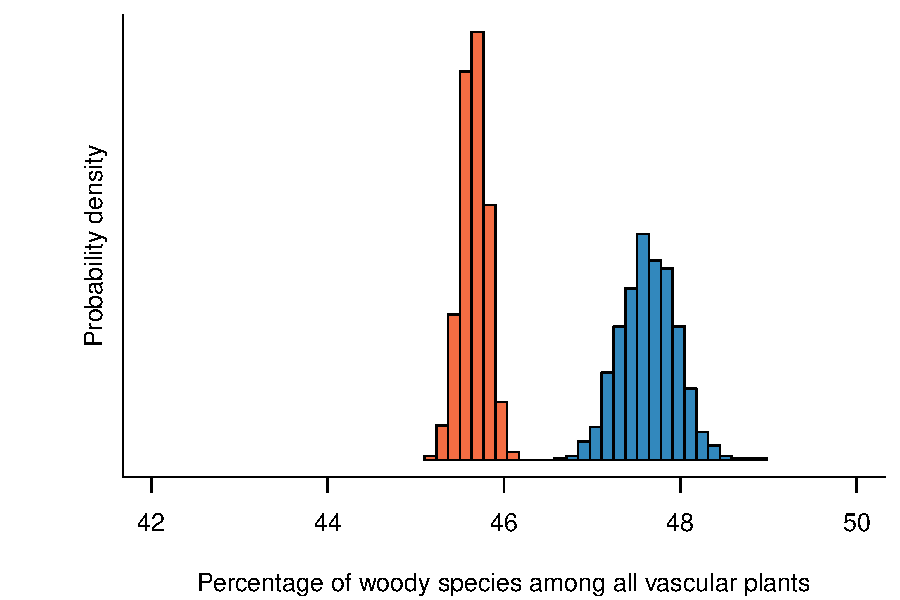
\includegraphics[width=\textwidth]{figs/distribution-raw}
  \caption[Estimates of woodiness proportion using alternative sampling
  approaches]{The posterior probability distribution for
    the proportion of the world's flora that is woody, using our two
    sampling approaches.  The red (left) distribution samples missing
    species using the strong prior approach (binomial distribution),
    while the blue distribution (right) samples missing species using
    the weak prior approach (hypergeometric distribution).}
  \label{fig:distribution-raw}
\end{figure}


The different approaches generated different distributions of the
per-genus percentage of woodiness (Fig.
\ref{fig:distribution-genera}), with a less strongly bimodal
distribution using the weak prior approach. (See Figs.
\ref{fig:distribution-family} and \ref{fig:distribution-order} 
for the distributions at the level of families and orders, respectively.) 
However, the two different approaches (strong
versus weak priors) led to similar phylogenetic distributions of
estimated woodiness (Fig. \ref{fig:phylogeny} versus Fig.
\ref{fig:phylogeny-supp}), differing only in the details. We have compiled
a table of the estimated number of woody species under both sampling
approaches for all genera, families and orders included in our analysis.
This is included in the Supplementary Material and is available on the 
Dryad data repository \citep[doi:10.5061/dryad.v7m14]{FitzJohnDryad}.

\begin{figure}[p]
  \centering
  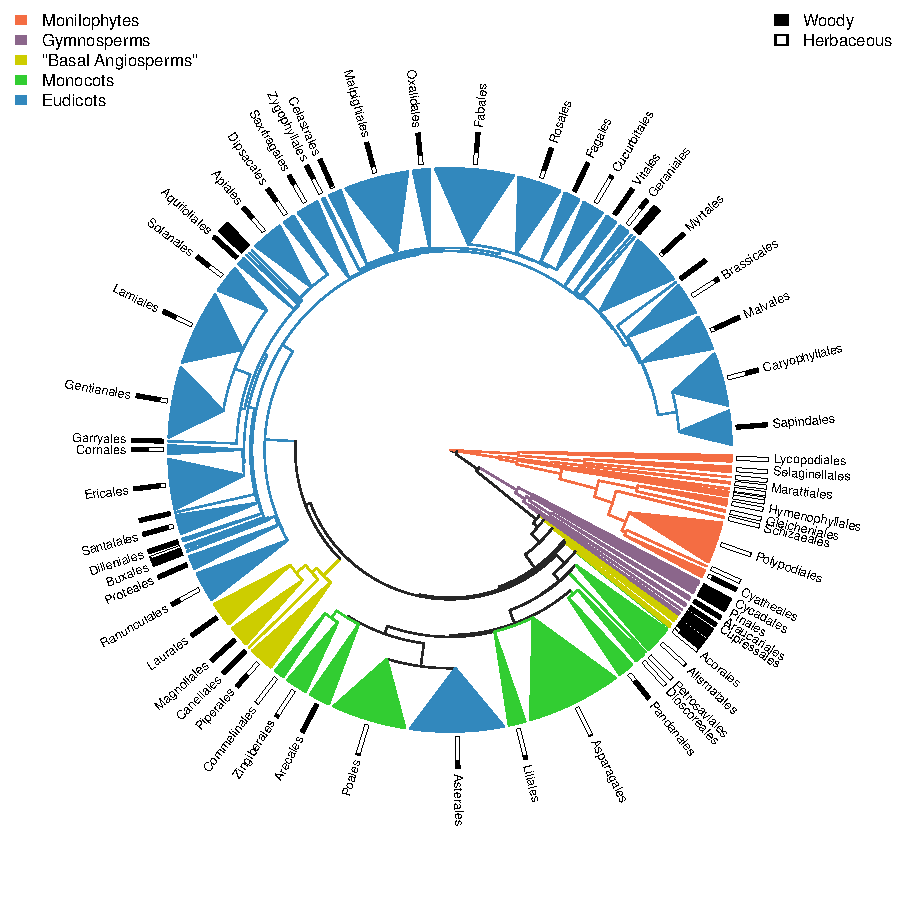
\includegraphics[width=\textwidth]{figs/fraction-on-phylogeny}
  \caption[Distribution of the fraction of woodiness among orders of vascular
  plants I]{Distribution of the percentage of woodiness among orders of
    vascular plants.  Each tip represents an order, with the width of
    the sector proportional to the square root of the number of
    recognised species in that order (data from accepted names in
    \citet{ThePlantList}).  The bars around the perimeter indicate the
    percentage of woody (black) and herbaceous (white) species,
    estimated using the ``strong prior'' (binomial) approach.  Using
    the ``weak prior'' (hypergeometric) approach generally leads to an
    estimated percentage that is closer to 50\% (see Figs.
    \ref{fig:phylogeny-supp} and \ref{fig:distribution-genera}).
    Phylogeny from \citet{Zanne} (available on Dryad; 
    doi:10.5061/dryad.63q27/3). Orders not placed by APG III
    \citep{APG3} are not displayed. We note that there is some discrepancy between
    the Zanne et al. tree and previous well-supported
    phylogenetic hypotheses \citep[e.g.,][]{Soltis2011}, most notably, in the
    position of the Magnoliids; however, the higher-level relationships 
    do not influence any of the analyses.}
\label{fig:phylogeny}
\end{figure}

\begin{figure}[p]
  \centering
  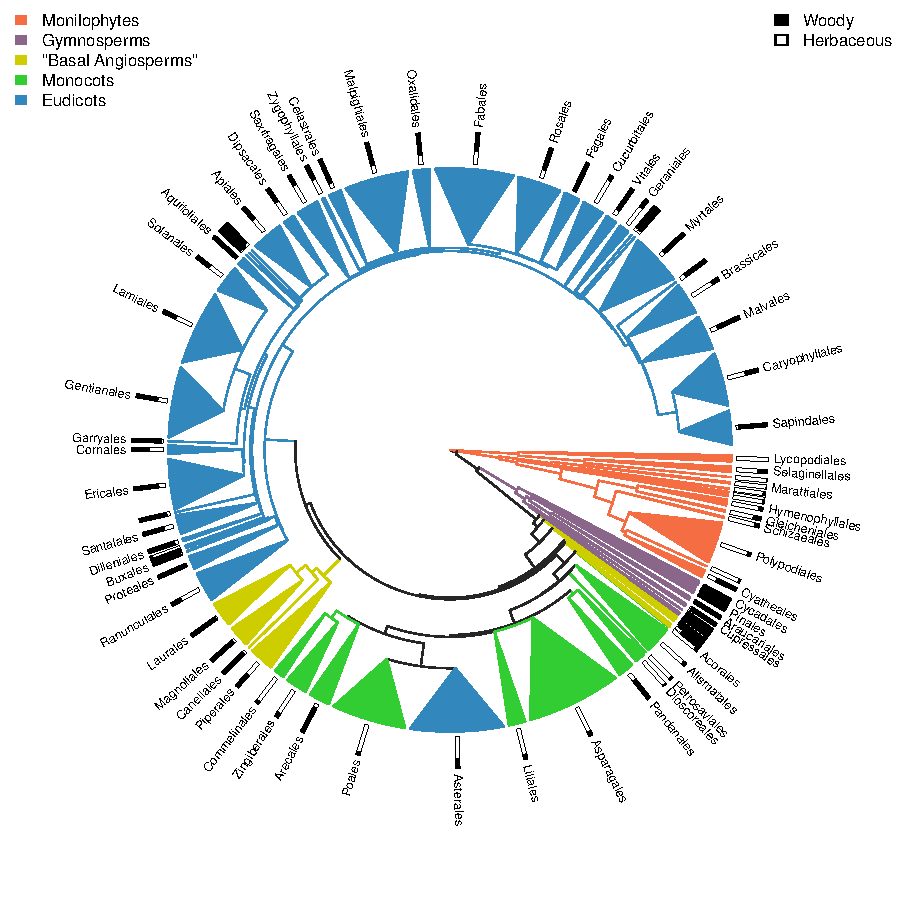
\includegraphics[width=\textwidth]{figs/fraction-on-phylogeny-supp}
  \caption[Distribution of the fraction of woodiness among orders of vascular
  plants II]{%
    Distribution of the fraction of woodiness among orders of vascular
    plants.  Each tip represents an order, with the fraction of
    circumference proportional to the square root of the number of
    recognised species in that order (data from accepted names in
    \citet{ThePlantList}).  The bars around the perimeter indicate the
    percentage of woody (black) and herbaceous (white) species,
    estimated using the ``weak prior'' (hypergeometric) approach.
    Using the ``strong prior'' (binomial) approach generally leads to
    an estimated percentage that is further away from 50\% (see
    main text Figs. 1 and 2).
    Phylogeny from \citet{Zanne} (available on Dryad;
    doi:10.5061/dryad.63q27/3). Orders not placed by APG III
    \citep{APG3} are not displayed.}
  \label{fig:phylogeny-supp}
\end{figure}

As stated above, neither of these sampling approaches is ``correct''. However,
as the observed distribution of woodiness fraction among genera is
itself strongly bimodal, we believe that the true result lies closer
to 45\% than to 47\%.  A more sophisticated hierarchical modelling
approach could lead to a more precise answer, but we feel that our
values probably span the range of estimates that such an approach
would generate. And in any case, we felt that addressing a simple question
warranted a simple approach.  

% #rstats
% n.spp <- sum(res.b$order$N)
% res <- list(b=res.b,h=res.h,b.w=res.b.w,h.w=res.h.w,b.h=res.b.h,h.h=res.h.h)
% tmp <- do.call(rbind, lapply(res, function(x) x$overall/n.spp)) * 100
% tmp2 <- round(tmp, 2)
% c(tmp["b.w",1], tmp["h.w",1]) - c(tmp["b",1], tmp["h",1])
% tmp["b.h",] - tmp["b",]
Different codings of variable species (see above) significantly moved
our estimates, despite affecting a small minority of species.  Coding
all variable species as woody, our estimates
% #rstats
% round(tmp["b.w",] - tmp["b",], 2)
% round(tmp["b.w",], 2)
increased by 1.6\% to 47.1\% with the strong prior approach
% #rstats
% round(tmp["h.w",] - tmp["h",], 2)
% round(tmp["h.w",], 2)
and by 1\% to 48.6\% with the weak prior approach (Fig.
\ref{fig:distribution-raw-errors}). Similarly, with coding
all variable species as herbaceous, the fraction of woody species
% #rstats
% round(tmp["b.h",] - tmp["b",], 2)
% round(tmp["b.h",], 2)
decreased by 1.9\% to 43.7\% under a strong prior
% #rstats
% round(tmp["h.h",] - tmp["h",], 2)
% round(tmp["h.h",], 2)
and by 1.3\% to 46.3\% under a weak prior (Fig.
\ref{fig:distribution-raw-errors}).

\begin{figure}[p]
  \centering
  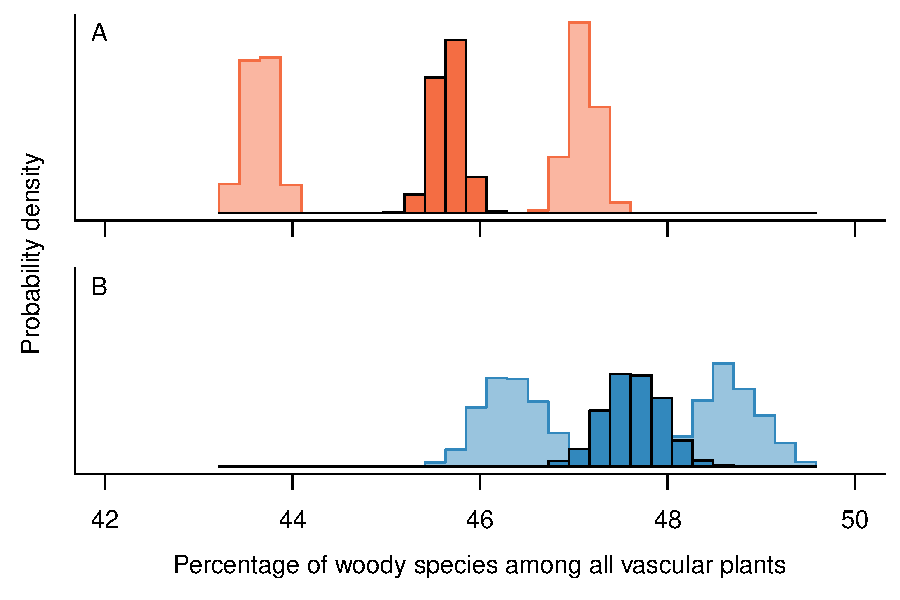
\includegraphics[width=\textwidth]{figs/distribution-raw-errors}
  \caption[The effect of different coding on estimates]{The effect of
    different coding on estimates of the fraction of species that are
    woody, under the strong prior approach (binomial; panel A) and
    weak prior approach (hypergeometric; panel B).  The dark
    distributions are the results from our main analysis
    (Fig. \ref{fig:distribution-raw}).  Distributions to the left
    (with lower estimates of woodiness) code all species with any
    record of herbaceousness or variability as herbaceous.  Similarly,
    distributions to the right (with higher estimates of woodiness)
    code all species with any record of woodiness or variability as
    woody.}
  \label{fig:distribution-raw-errors}
\end{figure}

There was strikingly little consensus among researchers as to the
percentage of species that are woody.  We received 292 responses from
29 countries, with estimates that ranged from 1\% to 90\% with a mean
of 31.7\% (Fig. \ref{fig:survey-distribution}).  The lowest
estimate from our analyses (45\% woody) is greater than 81\% of our survey estimates.

% #rstats
% nrow(d.survey)                   # 292
% length(unique(d.survey$Country)) #  29
% range(d.survey$Estimate) # 1 - 90
% mean(d.survey$Estimate)  # 31.7
% mean(d.survey$Estimate < 45) # 0.81
% mean(d.survey$Estimate < 100*res.b$overall.p[["mean"]]) # 0.83
We found little effect of respondents' level of training on their
estimate (Fig. \ref{fig:survey}).  There was a significant effect of
the respondent's familiarity with plants on the estimates, primarily
driven by respondents with little botanical familiarity (the ``What's
a Plant?'' category in the survey), whose estimates tended to be lower (less woody)
than the estimates of those with more familiarity. However, excluding
respondents with little familiarity with plants had virtually no effect
on the mean estimate of respondents (32.4\% excluding this category as compared
to 31.7\% with them included).
% #rstats
% i <- !is.na(d.survey$Familiarity) & d.survey$Familiarity != "What's a Plant?"
% mean(d.survey$Estimate[i])
Restricting survey responses to only respondents at least ``Familiar''
with plants, and with at least an undergraduate degree in botany or a
related field (143 responses), only increased the mean survey estimate
to 32.9\%.
% #rstats
% i <- d.survey$Familiarity <= "Familiar" &
%     d.survey$Training <= "Undergraduate degree in botany or a related field"
% i[is.na(i)] <- FALSE
% sum(i) # 143
% mean(d.survey$Estimate[i]) # 32.9%

\begin{figure}[p]
  \centering
  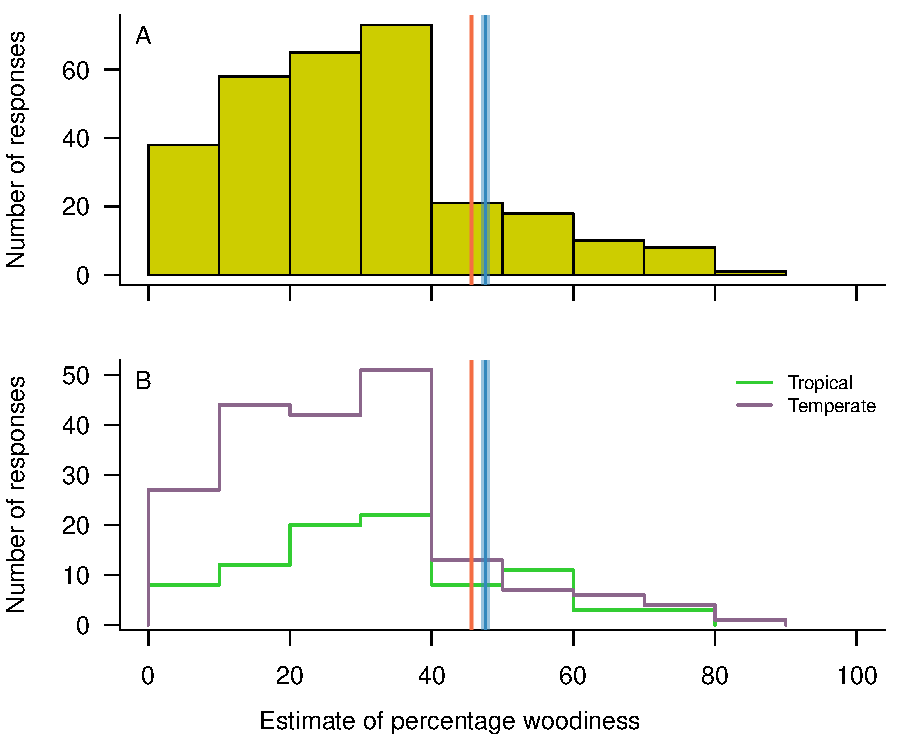
\includegraphics[width=\textwidth]{figs/survey-distribution}
  \caption[Distribution of survey responses]{Distribution of all
    responses to the survey question ``What percentage of the world's
    vascular plant species are woody?''.
    %
    The mean and 95\% confidence intervals for our estimates of the
    proportion of woody species from the empirical data are depicted
    by the horizontal shaded rectangles; the blue rectangle
    corresponds to the ``weak prior'' approach and the red rectangle
    corresponds to the ``strong prior'' approach (see Appendix for
    details).  
    % 
    Panel A includes all 292 responses.  In panel B, the 282
    responses that indicated country are shown separated into
    ``tropical'' (orange distribution) and ``temperate'' (teal).
    Estimates from tropical countries were slightly, but
    significantly, higher than those from temperate countries
    ($p=$0.02, $r^2$=0.02).
    % #rstats
    % nrow(d.survey)                   # 292
    % sum(!is.na(d.survey$Country))    # 282
    % summary(res.tro)
  }

  \label{fig:survey-distribution}
\end{figure}

\begin{figure}[p]
  \centering
  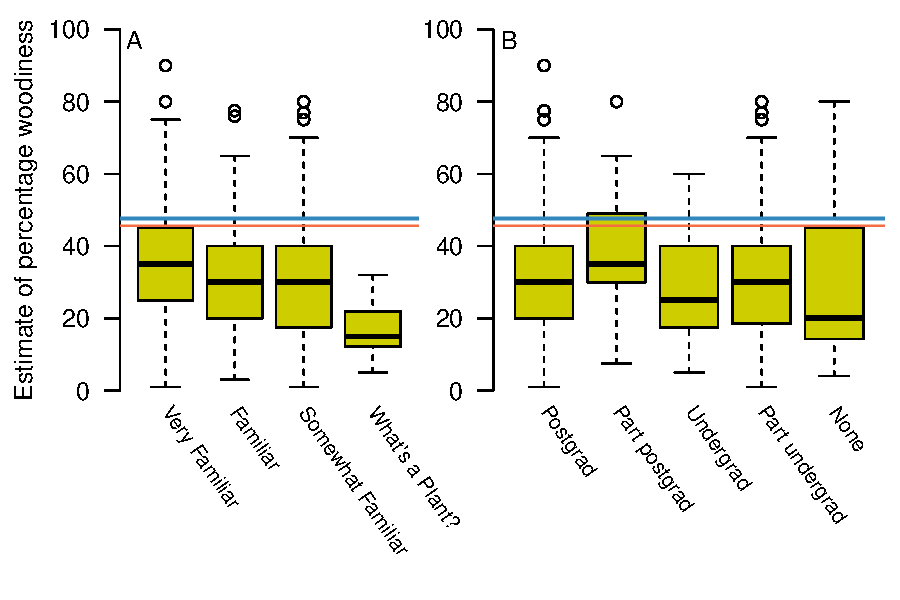
\includegraphics[width=\textwidth]{figs/survey-results}
  \caption[Survey results by familiarity and training]{Distribution of responses to the survey question ``What
    percentage of the world's vascular plant species are
    woody?''. Responses are divided by familiarity with plants
    (panel A) and formal training in botany or a related discipline
    (panel B). The mean and 95\% confidence intervals for our
    estimates of the proportion of woody species from the empirical
    data are depicted by the horizontal shaded rectangles; the blue
    upper rectangle corresponds to the ``weak prior'' approach and the
    red lower rectangle corresponds to the ``strong prior'' approach
    (see Appendix for details).}
  \label{fig:survey}
\end{figure}


Before carrying out the survey, we had hypothesised that researchers
from tropical regions may perceive the world as woodier than
researchers from more temperate regions due to the latitudinal
gradient in woodiness \citep{Molesheihgt}.
%
Indeed, there was an effect of being in a tropical country, with the
estimates from tropical countries being slightly higher than those
from temperate countries ($p$=0.02), but this effect was very small
($r^2$=0.02, Fig. \ref{fig:survey-distribution}).
% #rstats
% summary(res.tro)

\section{Discussion}

Our estimates of woodiness differed from both the survey and the
simple mean of the global database: neither simple statistics nor
biologists' intuition were accurate in this case.  The difference from
community knowledge is in striking contrast to \citet{joppa2010}, who
found that that expert opinion on the number of species within
different Angiosperm groups agreed closely with results based on
analyses of data and their bias.

The respondents to our survey perceived there to be substantially
fewer woody species in the world than there probably are.  This
herb-centric view of the world may arise from the importance of our
(mostly herbaceous) cultivated crops, or the fact that people --
including most researchers--likely spend more time in the garden than in
the forest, and especially not in tropical forests where diversity is high and disproportionately woody.

Our estimates of the percentage of species that are woody (45/48\%)
differ from the raw estimate based on species in our database (59\%).
This difference is caused by the interaction between biased sampling
and clustered trait data at a variety of taxonomic scales.
% #rstats
% round(100*range(c(res.b$overall.p, res.h$overall.p))) # [45,48]
% sum(dat.g$W) / sum(dat.g$K) # 0.59 - fraction
The distribution of woodiness is bimodal among genera, and the
distribution of sizes of those genera differs with woodiness.  Genera
that are primarily herbaceous (less than 10\% woody species for genera
with at least 10 records) were on average larger than primarily woody
genera (more than 90\% woody species), with a mean of 214 species
compared to 151 (See Fig. \ref{fig:variability}).
% #rstats
% dat.10 <- dat.g[dat.g$K > 10,]
% round(mean(dat.10$N[dat.10$p < .1])) # 214
% round(mean(dat.10$N[dat.10$p > .9])) # 151
This means that even a random sampling above the level of species will
lead to a biased estimate.

\begin{figure}[p]
  \centering
  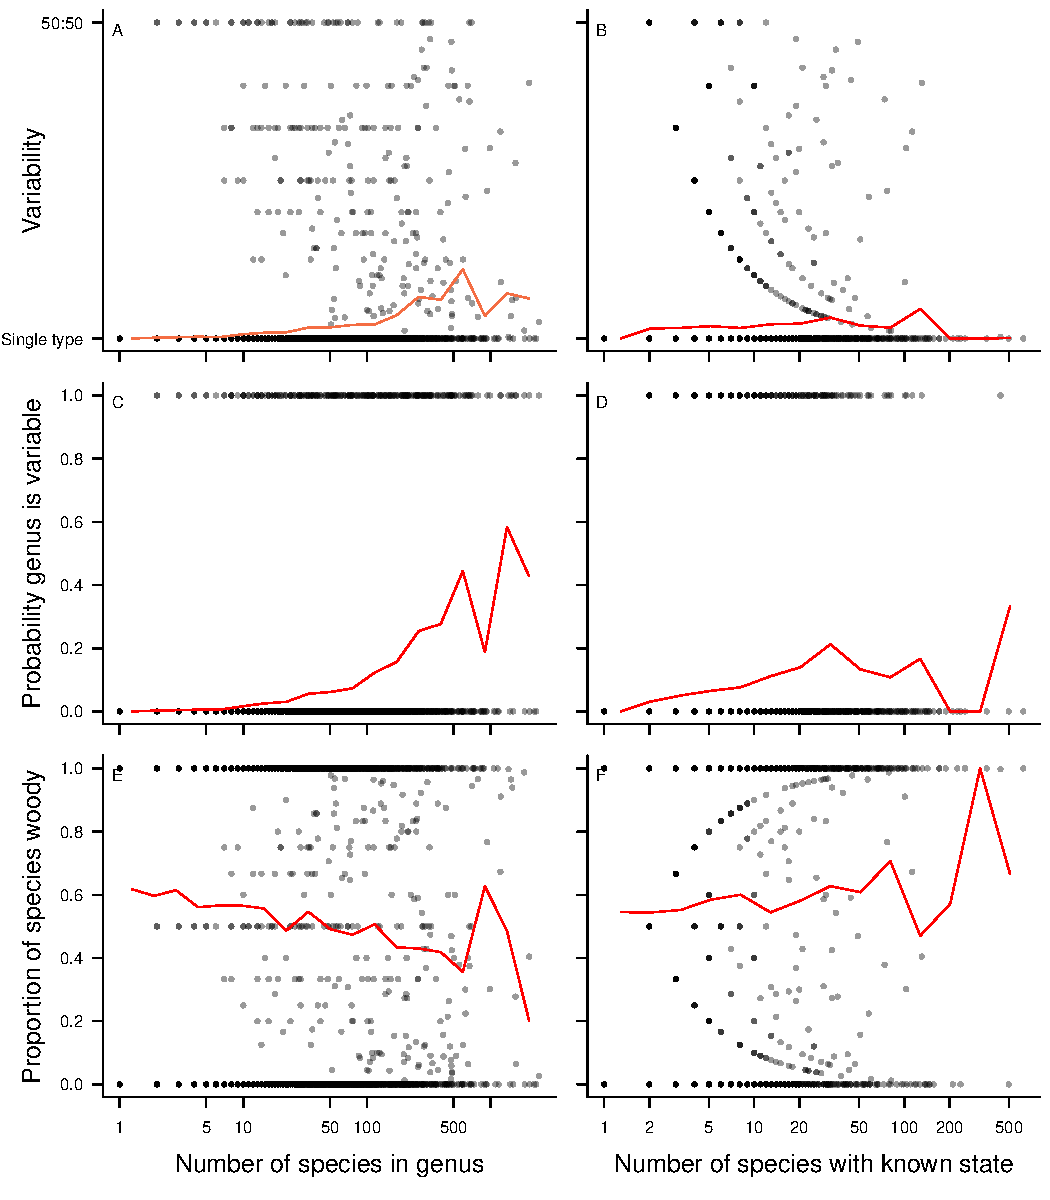
\includegraphics[width=.8\textwidth]{figs/variability}
  \caption[Relationship between genus size and proportion of
  woodiness]{The relationship between the size of a genus and its
    chance of being ``variable'' for woodiness.
%
We plotted the relationship between the level of variablitiy in the
dataset (from all of a single--type to equal numbers of woody and
herbaceous species) against the number of species in a genus (panel A)
and the number of species with known state (panel B). Larger genera
tend to be more variable although this pattern is not strong. We then
coded all genera as being either variable or all of a single--type and
examined the relationship between this binary characterization and the
number of species per genus (panel C) and the number for which we
have known states (panel D). Using the binary characterization, it is
clear that large genera have a higher probability of being variable,
even if few species actually vary (compare with panels A and
B). Though there is a great deal of scatter, larger genera also tend to be
more herbaceous than woody genera (panel E) but the genera for which
we have more data tend to be more woody (panel F). This shows that the
available data is generally biased towards woody species.  In all
panels, the red line is a moving average over 20 (left column) of 15 (right
column) equally spaced bins on this log axis.}
  \label{fig:variability}
\end{figure}

The effect of sampling bias within our database on the estimate is
amplified by the distribution of woodiness at higher taxonomic levels,
with families or even orders often being predominantly either woody or
herbaceous (Fig. \ref{fig:phylogeny} and
\citealt{sinnott1915evolution}).  There are two major clades that are
primarily herbaceous--the monocots (Monocotyledons) and ferns
(Monilophyta). However, there are many primarily herbaceous clades
nested within woody clades, and vice versa, which makes the
combination of taxonomic and functional information crucial for
answering this type of question.

We also found that the way in which we handled variable species
significantly altered the estimates. That changing the state of such a
relatively small number of species has the potential to alter
inferences made at a global scale is rather surprising. Two points
regarding this are worth noting here. First, we reiterate that our
alternate coding schemes (all variable species coded as herbaceous and
all variable species coding as woody) are rather extreme and unlikely
to be biologically realistic. Second, while these alternate coding
schemes certainly affected the estimates, the magnitude of their
effect is much less than that of the overall sampling bias in the
original database.

Higher-order classifications are at least as much a product of human
pattern matching as biological processes.  Genera correspond to the
morphological discontinuities among species that humans deem important
\citep{scotland2004significance}, which likely includes woodiness
\citep[e.g.,][]{Hutchinson}.  The relative rarity of genera with
significant numbers of both woody and herbaceous species (Fig.
\ref{fig:distribution-genera}) reinforces the importance of this
trait.  A significant, but unaccounted for, source of error is the
likely nonrandom woodiness of undiscovered species. We would predict
that there are likely more herbs to be discovered than woody plants;
larger genera tend to be more herbaceous (Fig. \ref{fig:variability}) and we
think it is more likely that new species are yet to be described in
these large groups.  In principle, rarefaction analysis could estimate
the number of species remaining to be discovered in different groups,
but this is not possible for many plant clades \citep{costello2011};
for many clades the ``collecting curve'' shows little sign of
saturation, which is required for such an analysis.

Sampling biases are pervasive in ecological datasets, and need to be
addressed when using them for analyses.  Global databases of
functional traits \citep[e.g., TRY;][]{kattge2011try} are central to
biodiversity research, but through no fault of the database collator
they are inevitably biased in terms of taxonomic breadth and this may
have serious consequences for the reliability of inferences drawn from
them.  For example, for woodiness the economic importance of forestry
species likely leads to their over-sampling in this dataset.
This sampling bias also affects many commonly used methods in
ecological and evolutionary research
\citep[e.g.,][]{ackerly2000taxon,nakagawa2008missing,PennellHarmon,Pakeman2013}
in addition to its well understood effects on conventional statistics.
In our case, taking the data at face-value, we would have greatly
overestimated the global percentage of woody species.  Inferring the
global frequency of any trait would face the same problem.  For
example, the ecologically important traits of nitrogen-fixing,
mycorrhizal symbioses and pollinator syndrome are strongly
taxonomically structured, and we would expect raw estimates to be
biased in the same way that woodiness was.  Our approach was developed
for binary traits but similar approaches could be developed for
multi-state categorical or continuous traits.

In addition to improving an estimate of the mean, the methods in this
chapter can also be used to generate a probability of each unobserved
species being woody.  Thus, it can be used as a type of taxonomically-informed 
data-imputation.  Recently, two related approaches have
been developed to do just this, both focusing on continuous traits
\citep{Swenson2013, PEM}.  While their details differ, both approaches
are model-based in that they impute trait values for missing species
based on the fitted parameters of phylogenetic models estimated from
the species already in the database. This is conceptually different
from our approach; we do not assume any model for the evolution of
woodiness, such as the `Mk' model \citep{Pagel1994}, which is commonly
used to model discrete characters evolving on a phylogeny. Both types
of approaches--using taxonomic categories (this study) versus
modeling trait evolution along a phylogeny--have advantages and
disadvantages.  One disadvantage of a modeling-based approach is that
if the sampling is biased with respect to the character states, the
parameter estimates themselves will be biased, leading to an incorrect
estimation of the states for the remaining species. While our approach
avoids this issue, we ignore potentially useful information on the
phylogenetic relationships within genera and branch lengths separating
lineages.

\section{Concluding remarks}

As a result of centuries of effort, we now have an increasingly
complete understanding of taxonomic diversity.  More recent
developments in assembling global trait databases offer the promise of
gaining similar insights into the functional diversity of the earth's
biota.
%
While the question we ask in this chapter--what proportion of the
world's flora is woody?--is simple, answering it required dealing
with the pervasive biases that will be present in most large datasets.
%
Researchers should be aware that because of these biases and the
phylogenetically structured distribution of traits, the law of large
numbers will not apply, and that estimates from trait databases will
not converge on the true value.
%
Our approach is just one of many potential ways to address these
biases; we hope that our analysis encourages others to think
critically and creatively about the problem.
%
Just as Theophrastus' garden was a non-random sample of the Greek
flora, our trait databases contain diverse biases; accounting for them
will be important in making inferences about broad-scale ecological
and evolutionary patterns and processes.


%\input{conclusion}

\formatbibliography
\bibliographystyle{refstyle}
\bibliography{refs-thesis}

%\formatappendices
%\input{anappendix}

\end{document}

%%% Local Variables:
%%% TeX-master: t
%%% TeX-PDF-mode: t
%%% End:
